\documentclass[12pt]{report}

\usepackage{mathtools}
\usepackage{amsmath}
\usepackage{systeme}
\usepackage{siunitx}
\usepackage[T1]{fontenc}
\usepackage{hyperref}
\usepackage{bigfoot}
\usepackage[numbered, framed]{matlab-prettifier}
\usepackage{filecontents}
\usepackage{graphicx}
\hypersetup{
colorlinks,
citecolor=black,
filecolor=black,
linkcolor=black,
urlcolor=black
linkto=all,
}

\newenvironment{simplechar}{%
   \catcode`\^=12
}{}

\title{Numerical Methods, project B, Number 32}
\author{Krzysztof Rudnicki\\ Student number: 307585 \\ Advisor: dr Adam Krzemieniowski}
\date{\today}

\let\ph\mlplaceholder % shorter macro
\lstMakeShortInline"

\lstset{
  style              = Matlab-editor,
  basicstyle         = \mlttfamily,
  escapechar         = ",
  mlshowsectionrules = true,
}

\begin{document}



\maketitle
\tableofcontents

\chapter{Find all zeros of function}

\section{a) False position method}

\subsection{Problem}

We have to find zeros of the function
\[ f(x) = -2.1 + 0.3x - xe^{-x} \]
In the interval $[-5; 10]$ using false position method.

\subsection{Theoretical Introduction}
\emph{False position} method also called \emph{regula falsi} in fancier circles is similar to the bisection method, the difference is that the interval we use $[a_n, b_n]$ is divided into two subintervals. We have:
\begin{itemize}
\item $\alpha$ - The root
\item $a_n$ - 'left' interval
\item $b_n$ - 'right' interval
\item $f(a_n)$ - Value at left interval
\item $f(b_n)$ - Value at right interval
\end{itemize}

We get:
\[ \frac{f(b_n) - f(a_n)}{b_n - a_n} = \frac{f(b_n) - 0}{b_n - c_n} \]
From which we get:
\[ c_n = b_n - \frac{f(b_n)(b_n - a_n)}{f(b_n) - f(a_n)} = \frac{a_nf(b_n) - b_n f(a_n)}{f(b_n)-f(a_n)} \]

Then we choose next interval as in the bisection method so: we calculate products of function values at $a_n$ and $b_n$ and that subinterval is selected for the next iteration of \emph{false position} method. This subinterval corresponds to the negative product value.

\subsubsection{Properties of \emph{false position method}}
This method is always convergent, simillary to bisection method, since it will always choose and shorten the interval which contains the root. If the function is continous and differentiable the method is linearly convergent. That being said the convergence may become sluggish. It can happen if for example one of the endpoints of the intervals will remain the same and the iterating will not shorten the interval to 0. One of the examples of functions that lead to that are barrier functions used in constrained optimization methods.

\paragraph{Improvement to the method}
In order to improve the formula and avoid aforementioned situation we can take smaller value of the function for the value that does not change.
For right end:
\[ c_n = \frac{a_n\frac{f(b_n)}{2} - b_nf(a_n)}{\frac{f(b_n)}{2} - f(a_n)} \]
And for left end:
\[ c_n = \frac{a_nf(b_n) - b_n\frac{f(a_n)}{2}}{f(b_n)- \frac{f(a_n)}{2}} \]

This is called \emph{modified regula falsi} or \emph{Illinois algorithm}.
It is superlinearly convergent, globally convergent and length of intervals we get in each iterations converges to zero.
\subsection{Results}

\begin{center}
   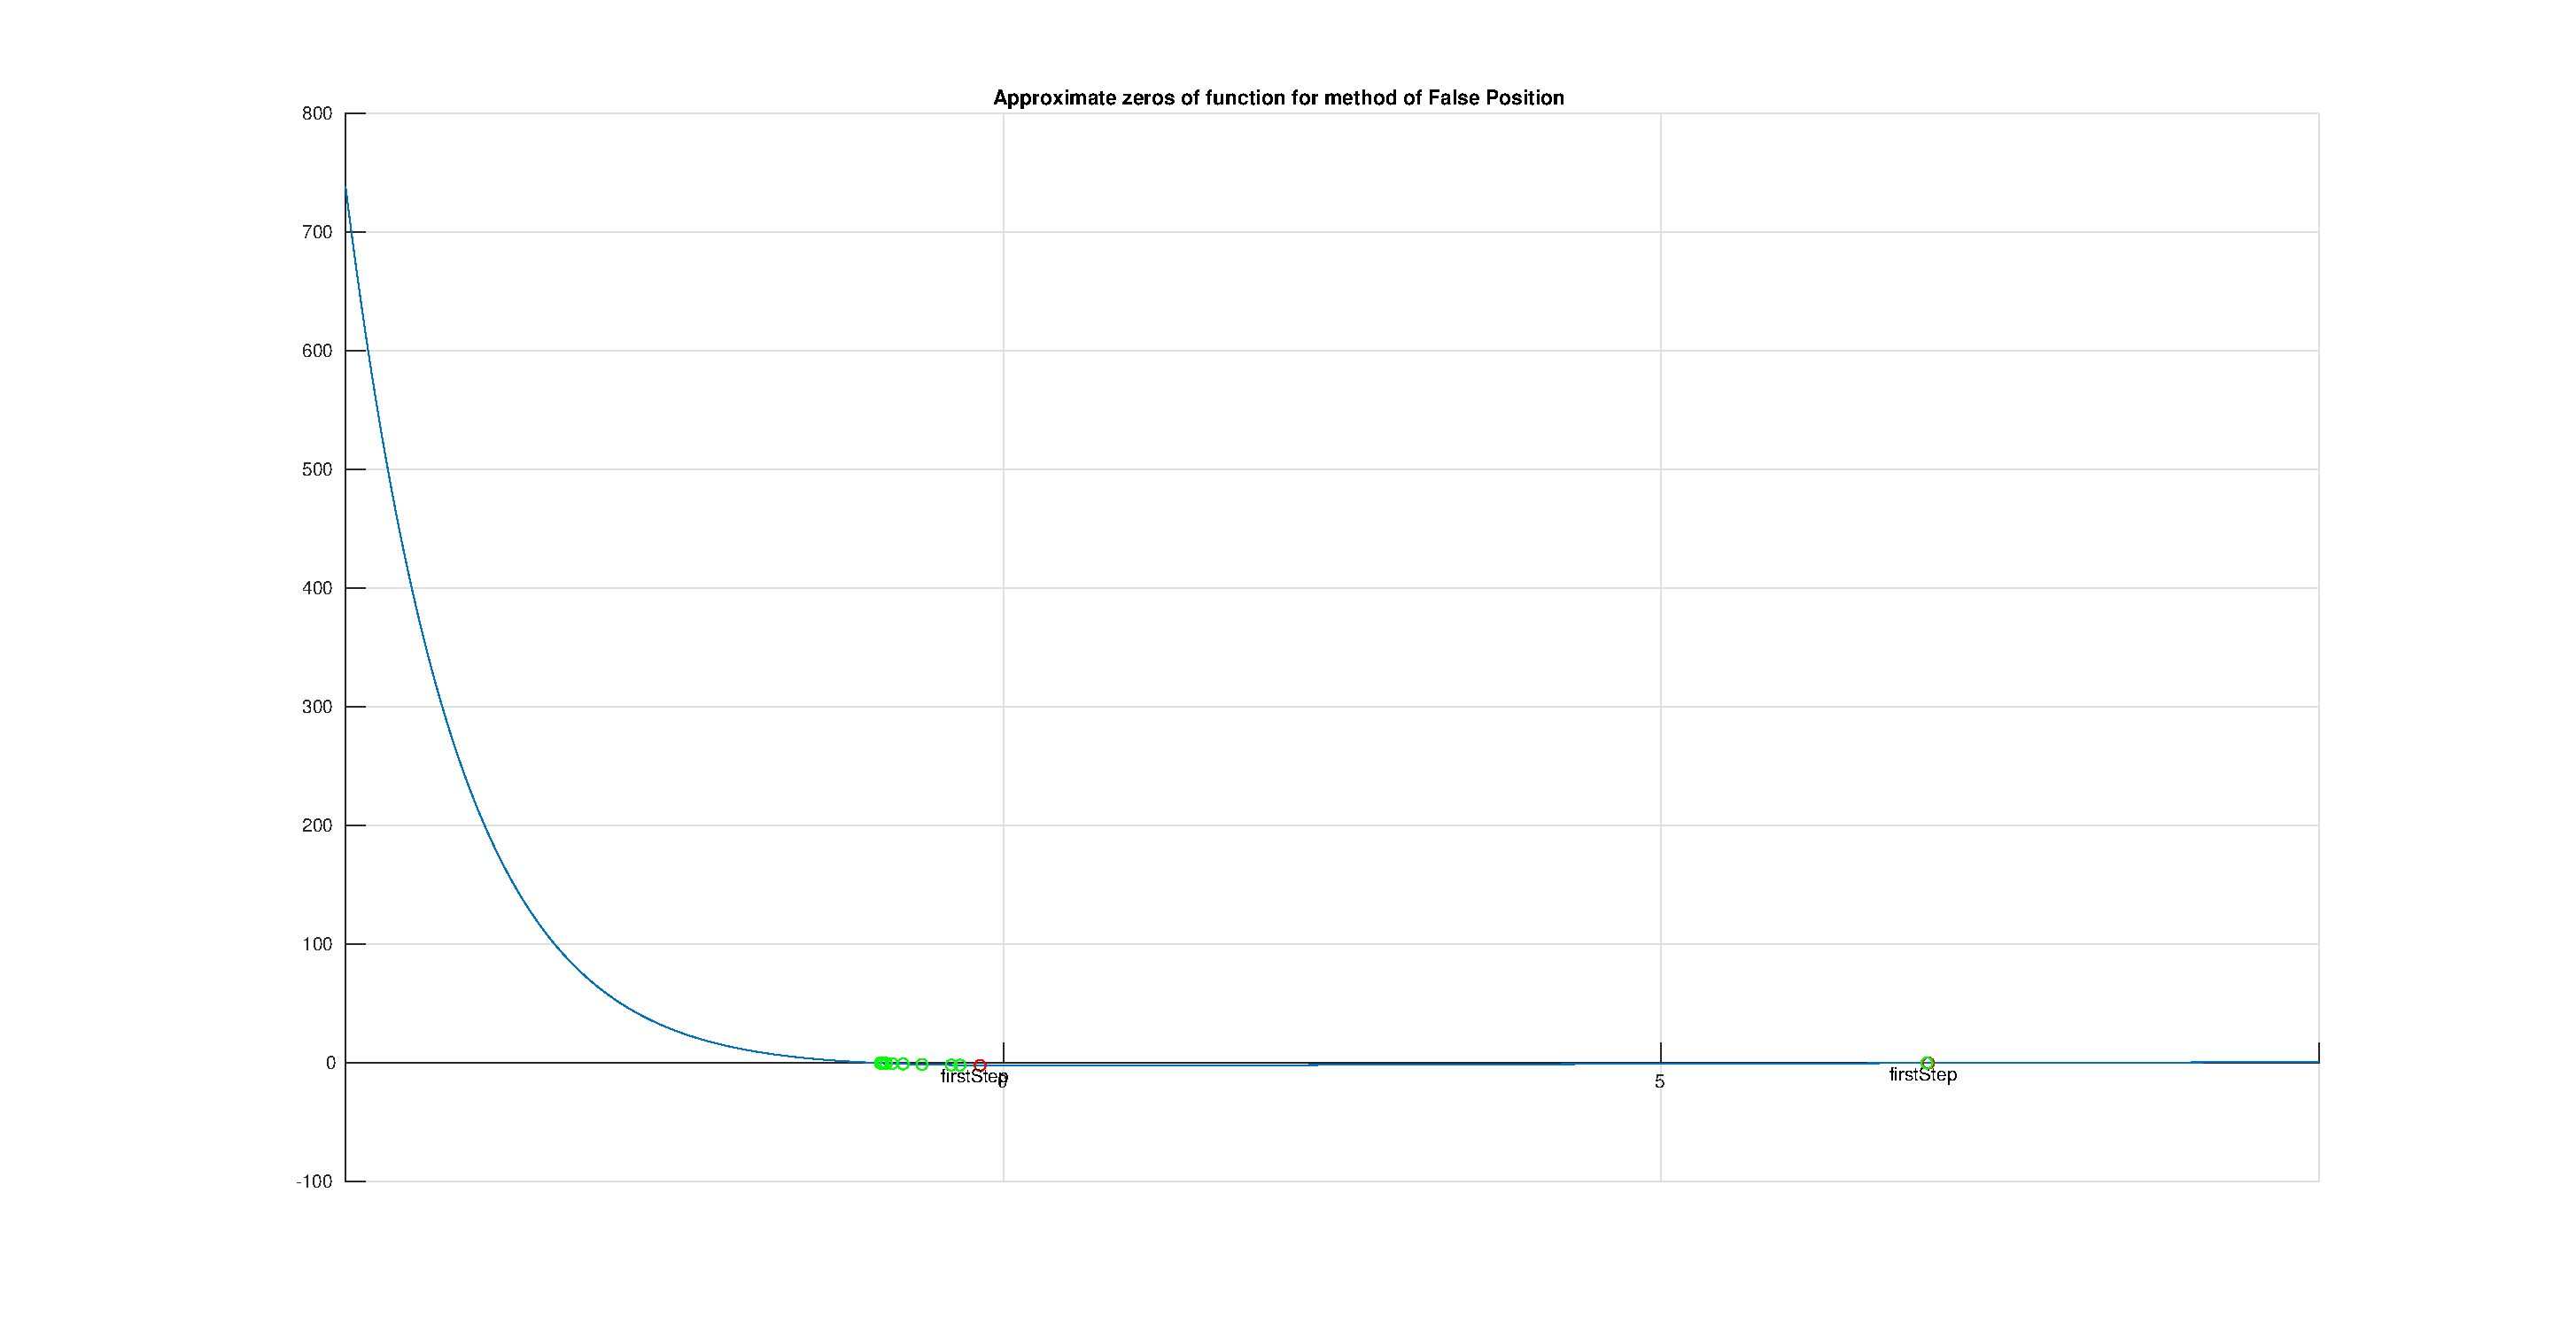
\includegraphics[scale=0.25]{task1falsepositionoverall.eps}
\end{center}

\begin{center}
   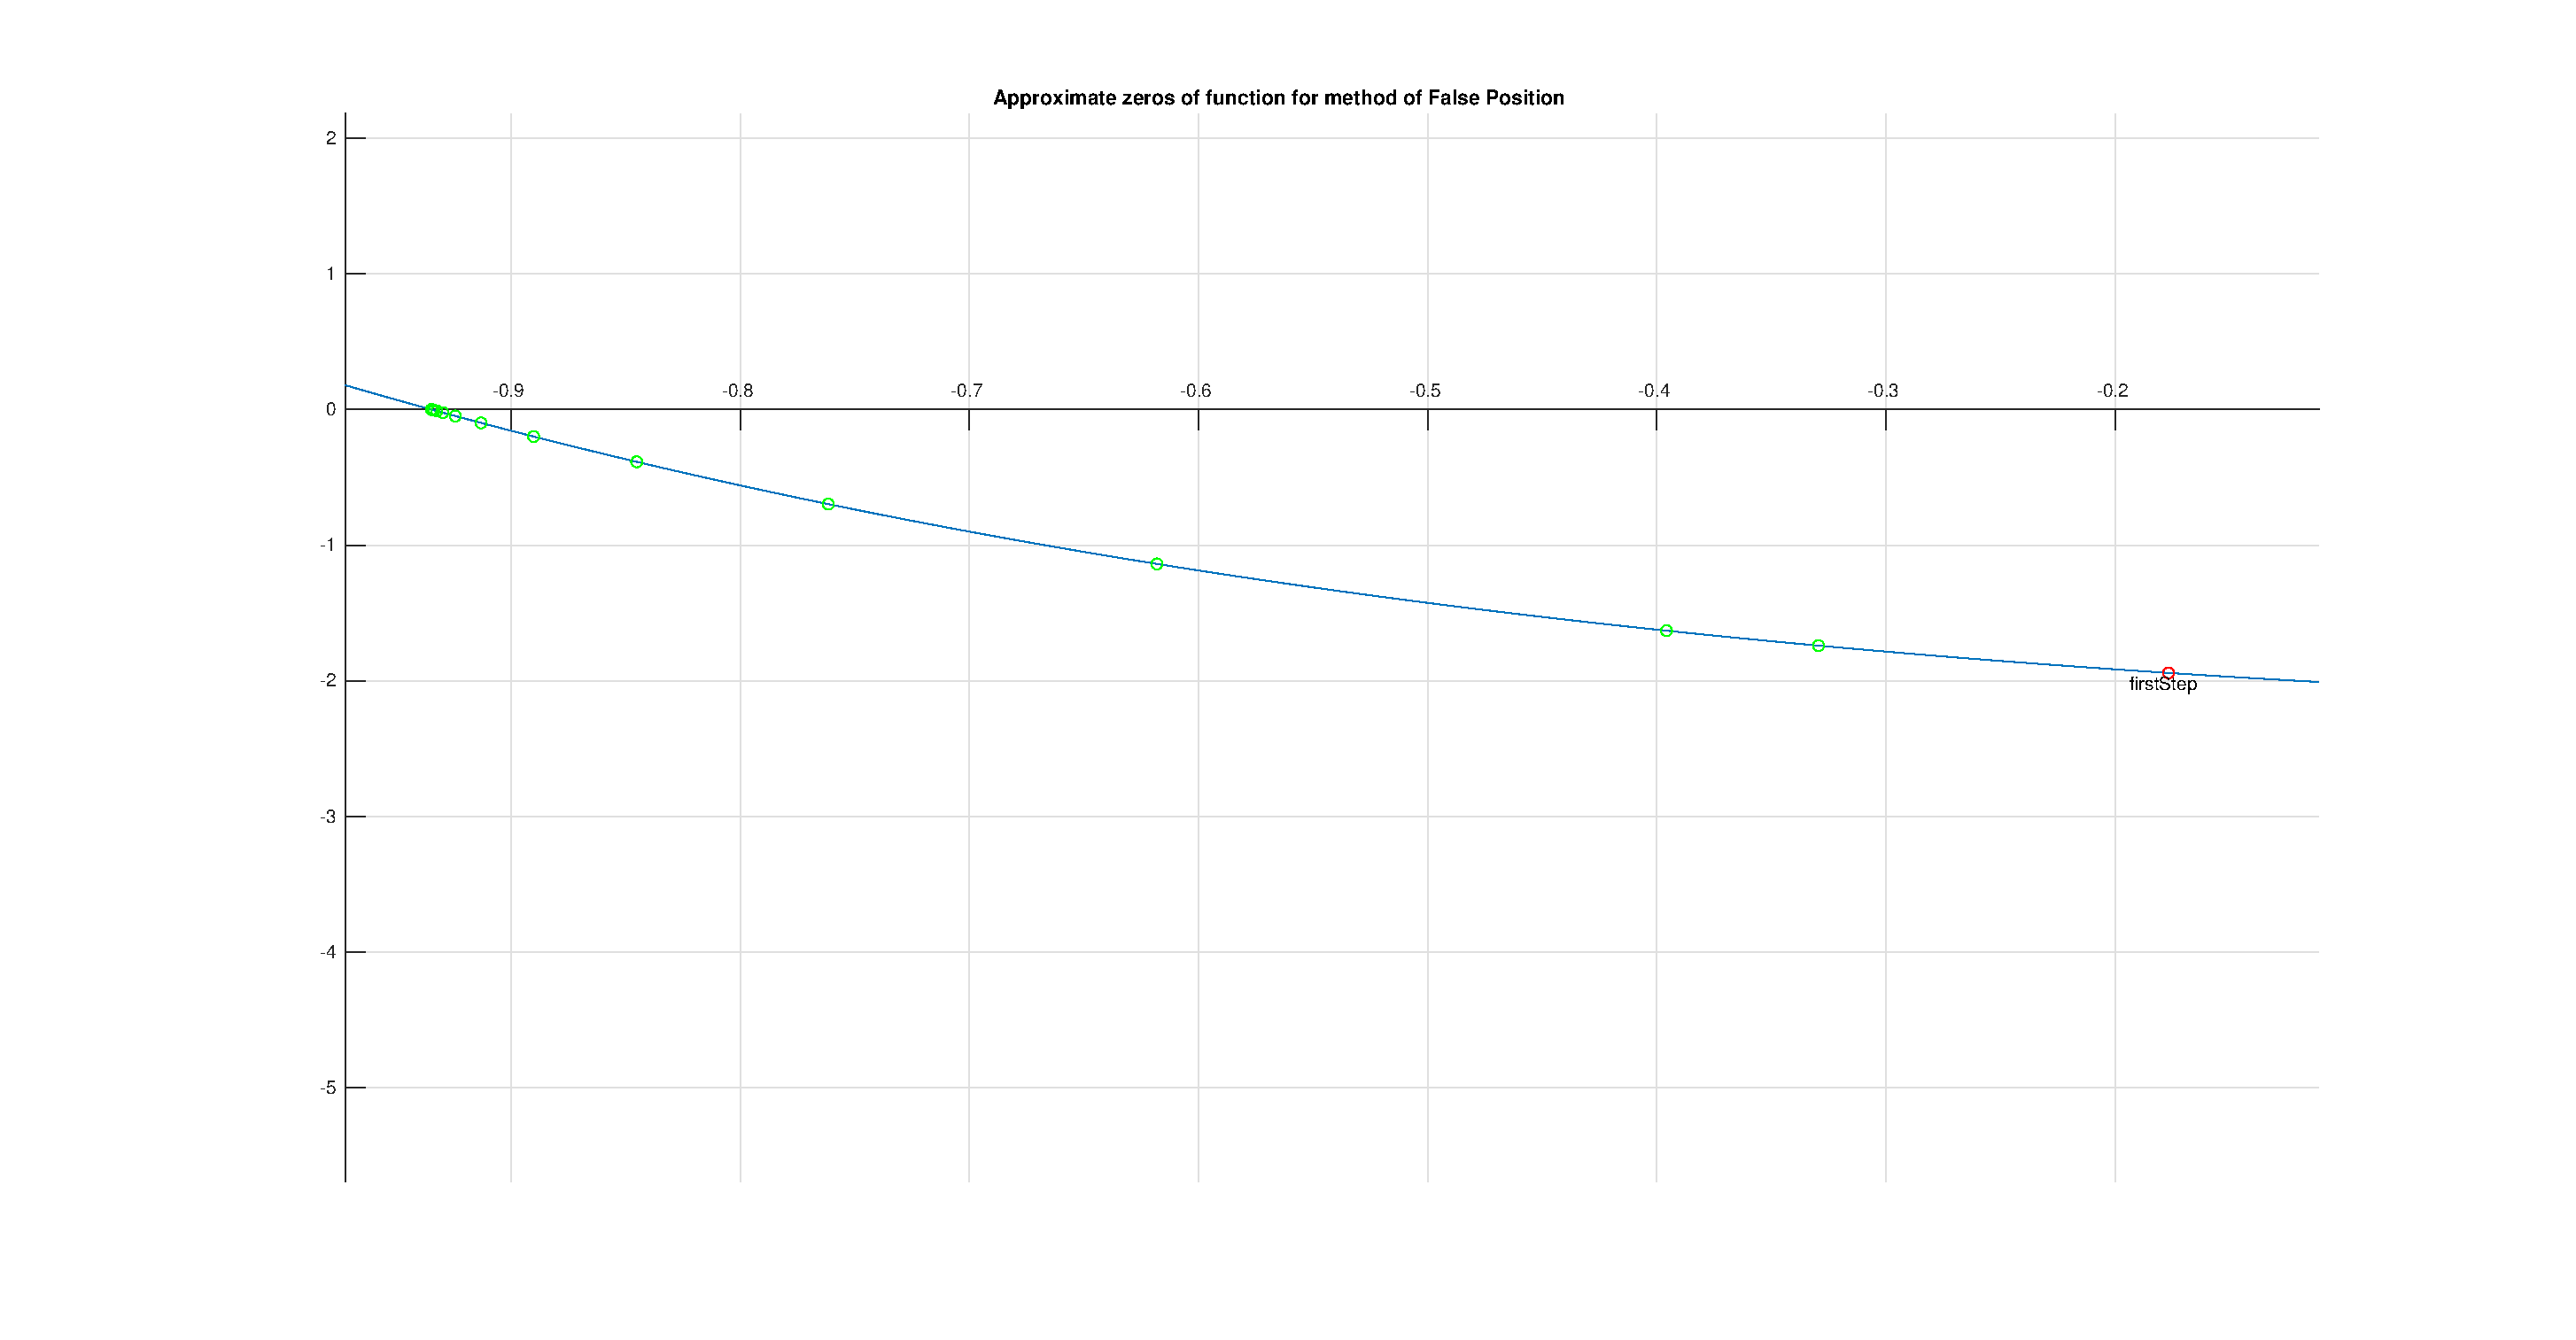
\includegraphics[scale=0.25]{task1falsepositionzommedleft.eps}
\end{center}

\begin{center}
   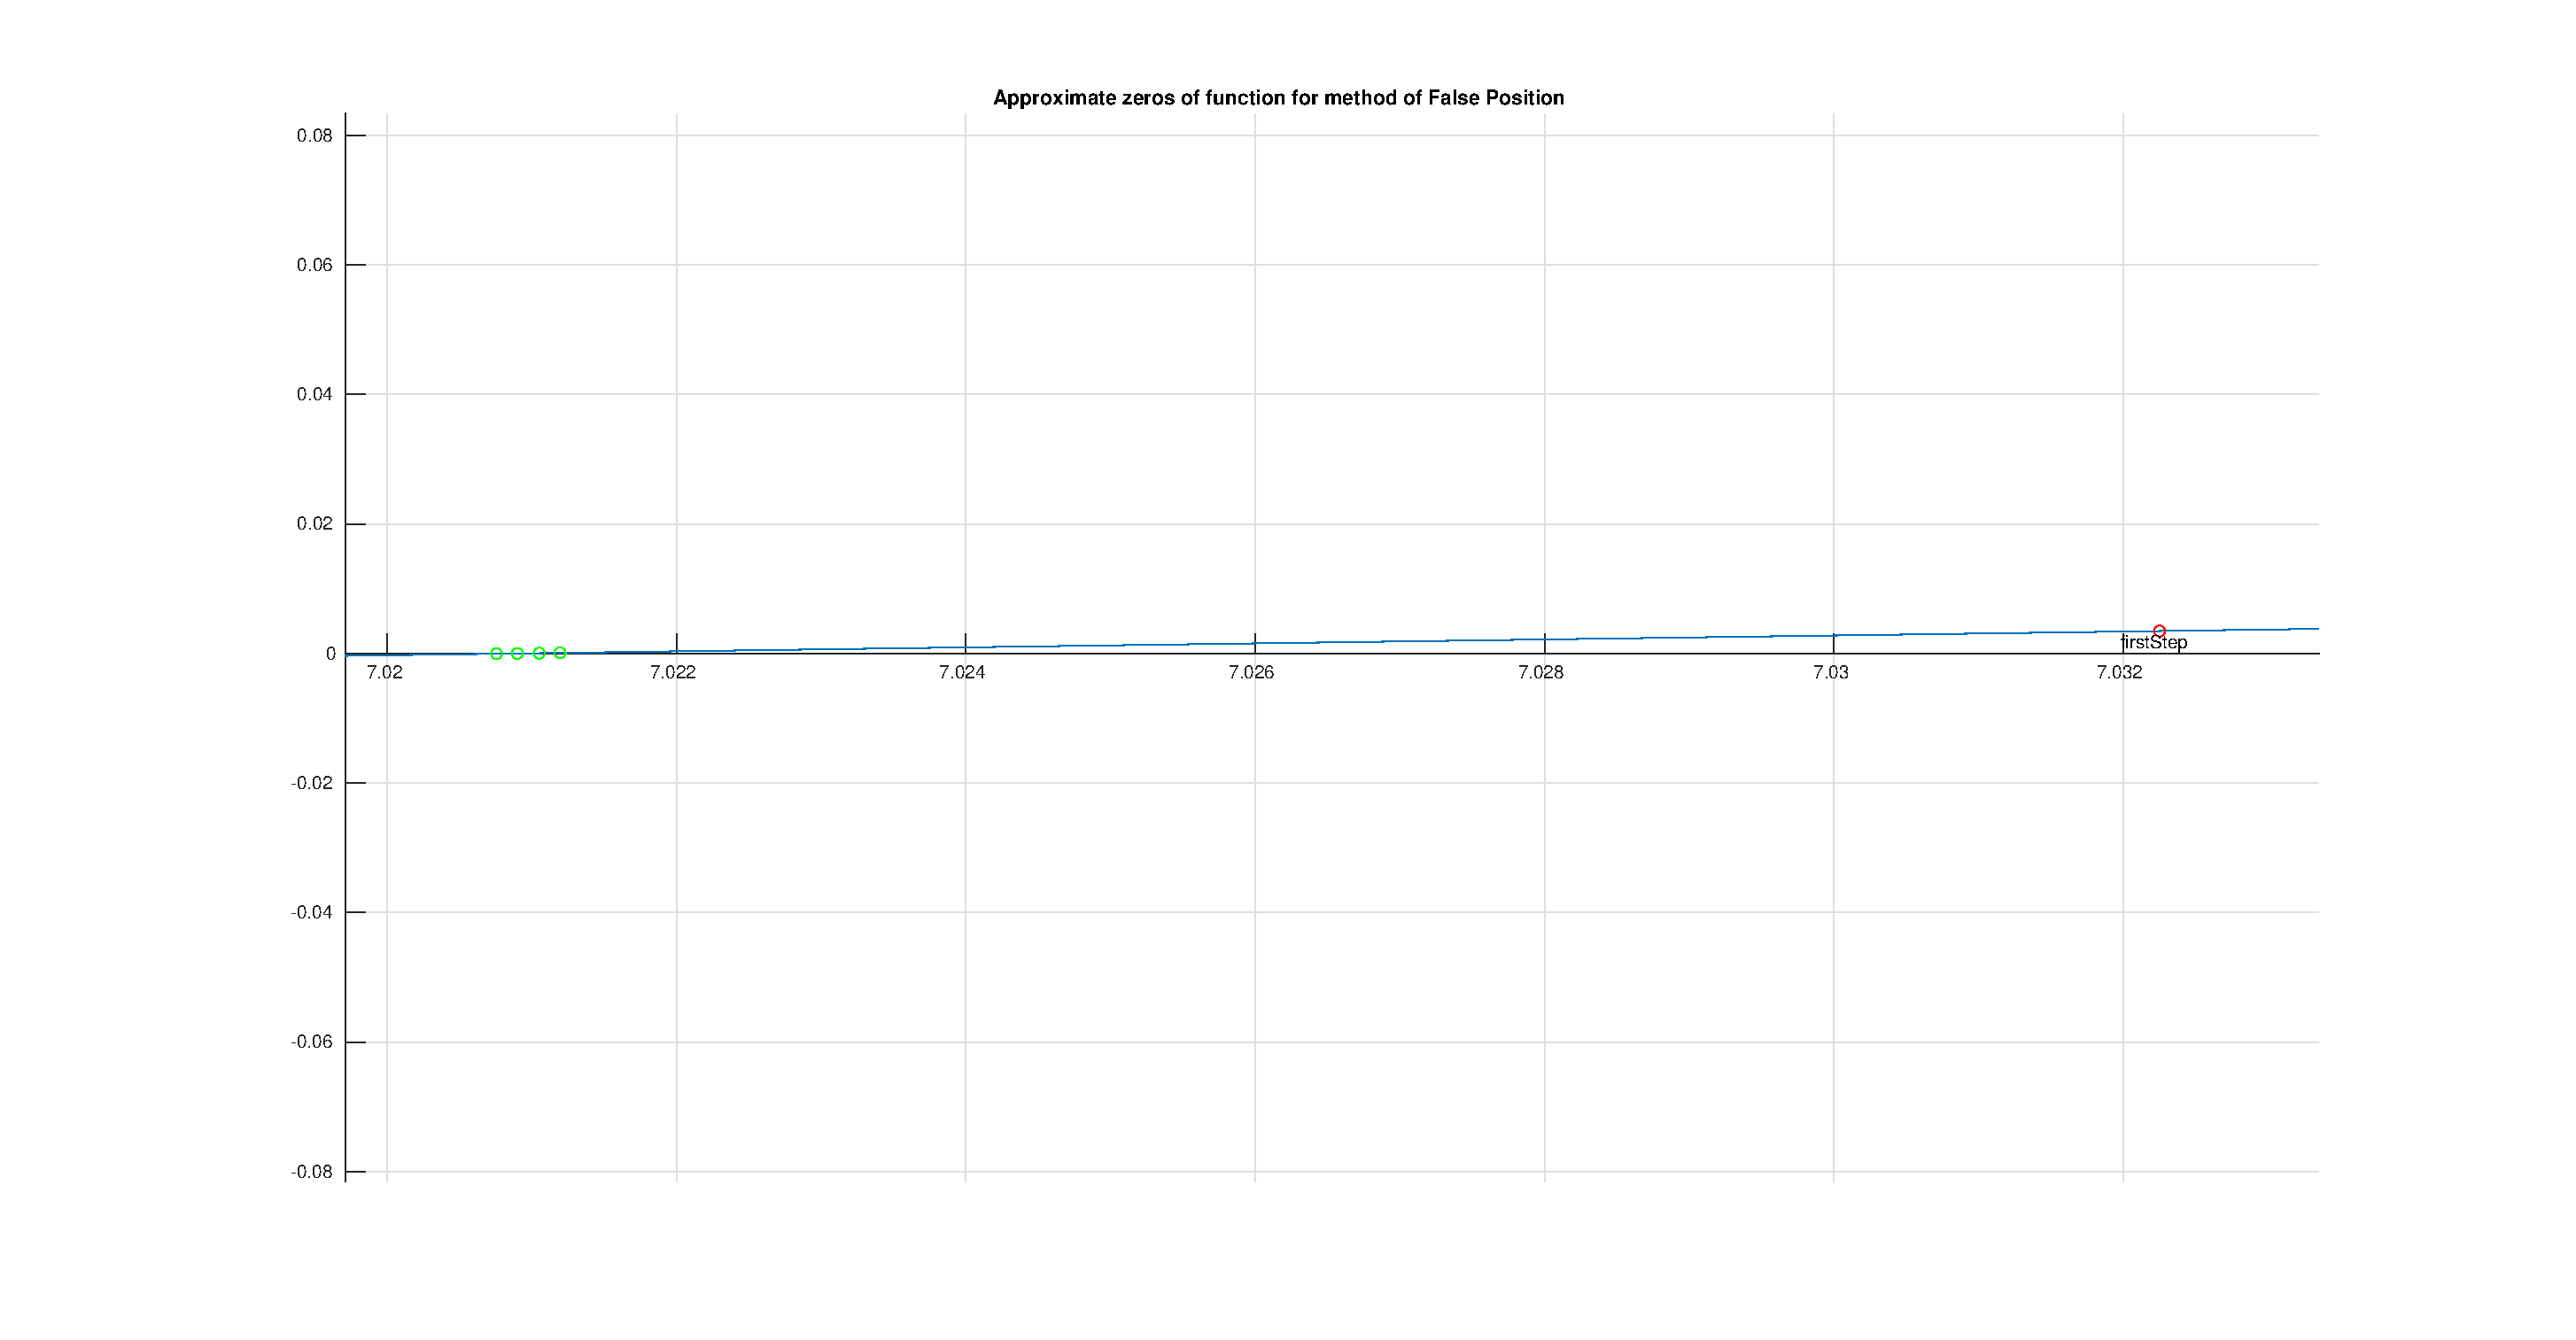
\includegraphics[scale=0.25]{task1falsepositionzommedright.eps}
\end{center}

\begin{center}
  \begin{tabular}{| c  c c |}
\hline
Iteration & root         & f(root) \\
\hline
1   &  -0.17673         &-1.9421 \\
\hline
2   &  -0.32943         &-1.7409 \\
\hline
3    & -0.39578         &-1.6308 \\
\hline
4     &-0.61812         &-1.1386 \\
\hline
5     &-0.76152        &-0.69765 \\
\hline
6     &-0.84516        &-0.38573 \\
\hline
7     &-0.89015        &-0.19911 \\
\hline
8     &-0.91304       &-0.098733 \\
\hline
9    & -0.92431       &-0.047922 \\
\hline
10    & -0.92976       & -0.02301 \\
\hline
11     &-0.93237       & -0.01099 \\
\hline
12     &-0.93362       &-0.005236 \\
\hline
13     &-0.93421      &-0.0024915 \\
\hline
14      &-0.9345      &-0.0011848 \\
\hline
15     &-0.93463      &-0.0005633 \\
\hline
16     &-0.93469     &-0.00026777 \\
\hline
17     &-0.93473     &-0.00012728 \\
\hline
18     &-0.93474     &-6.0499e-05 \\
\hline
19     &-0.93475     &-2.8756e-05 \\
\hline
20     &-0.93475    & -1.3668e-05 \\
\hline
21     &-0.93475    & -6.4964e-06 \\
\hline
22     &-0.93475    & -3.0878e-06 \\
\hline
23     &-0.93475    & -1.4676e-06 \\
\hline
24     &-0.93475    & -6.9758e-07 \\
\hline
25     &-0.93475    & -3.3157e-07 \\
\hline
26     &-0.93475    & -1.5759e-07 \\
\hline
27     &-0.93475    & -7.4906e-08 \\
\hline
28     &-0.93475    & -3.5603e-08 \\
\hline
29     &-0.93475    & -1.6922e-08 \\
\hline
30     &-0.93475    & -8.0433e-09 \\
\hline
31     &-0.93475    &  -3.823e-09 \\
\hline
32     &-0.93475    & -1.8171e-09 \\
\hline
33     &-0.93475    & -8.6368e-10 \\
\hline
34     &-0.93475    & -4.1051e-10 \\
\hline
35     &-0.93475    & -1.9512e-10 \\
\hline
36     &-0.93475    & -9.2741e-11 \\
\hline
\end{tabular}
\end{center}

\begin{center}
  \begin{tabular}{| c  c c |}
\hline
Iteration & root         & f(root) \\
\hline
1   &  7.0323         & 0.0034663 \\
\hline
2   &  7.0212          & 9.0344e-05 \\
\hline
3    & 7.0211         & 4.6349e-05 \\
\hline
4     & 7.0208        & -4.3921e-05  \\
\hline
5     & 7.0209        & 4.8939e-11  \\
\hline

\hline
\end{tabular}
\end{center}

\section{b) the Newton's method}


\subsection{Problem}

We have to find zeros of the function
\[ f(x) = -2.1 + 0.3x - xe^{-x} \]
In the interval $[-5; 10]$

using the Newton's method
\subsection{Theoretical Introduction}
\emph{The Newton's method} also called \emph{the tangent method} relies on first order part of its expansion into Taylor series for a given current approximation of root.
\[ f(x) \approx f(x_n) + f^{'}(x_n)(x-x_n) \]
Then we obtain the next point $x_{x+1}$ by finding root of linear function:
\[ f(x_n) + f^{'}(x_n)(x_{n+1}-x_n) = 0 \]
From this we get formula for $x_{n+1}$:
\[ x_{n+1} = x_n - \frac{f(x_n)}{f^{'}(x_n)} \]

This method as opposed to \emph{regula falsi} method is locally convergent, should we choose initial point too far from the root (area which is close enough to root is called set of attraction) then we can get a divergence. On the other side if the Newton's method will converge then it is quite rapid with convergence of order p = 2 - quadratic convergence.

Newton's method is also effective if the function derrivative is far from zero, so the slope of the function is steep, conversely if the derrivative is close to zero the method is not recommended.
\subsection{Results}

\begin{center}
   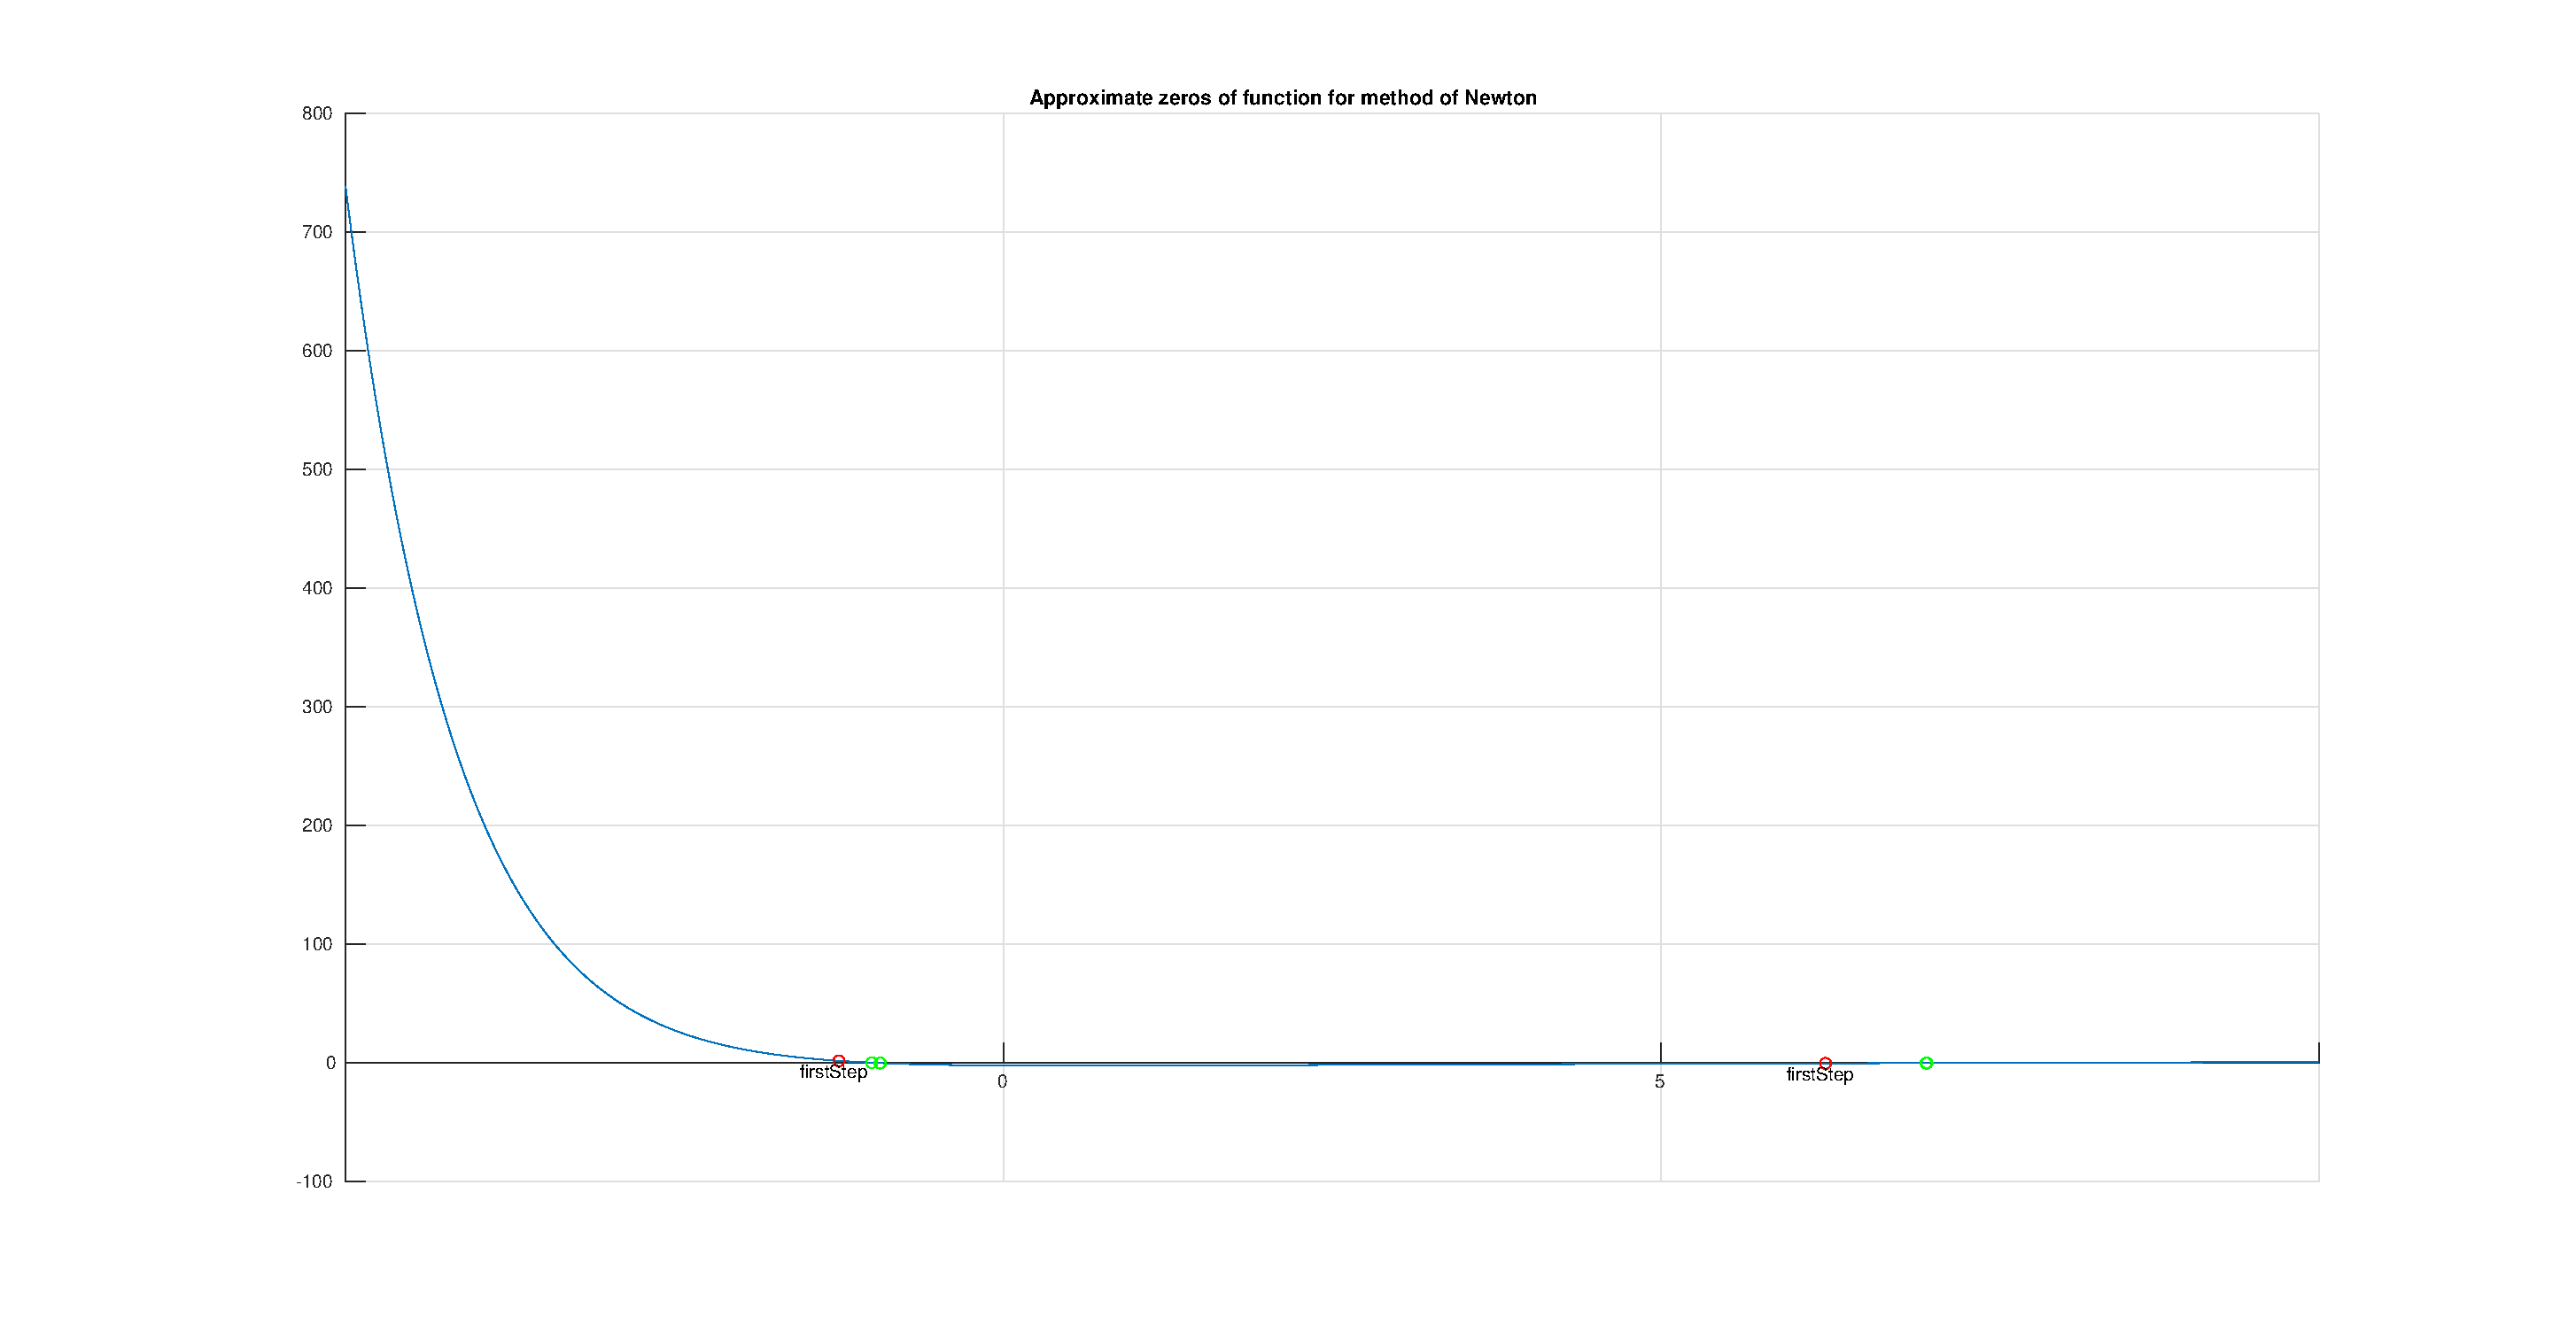
\includegraphics[scale=0.25]{task1Newtonoverall.eps}
\end{center}

\begin{center}
   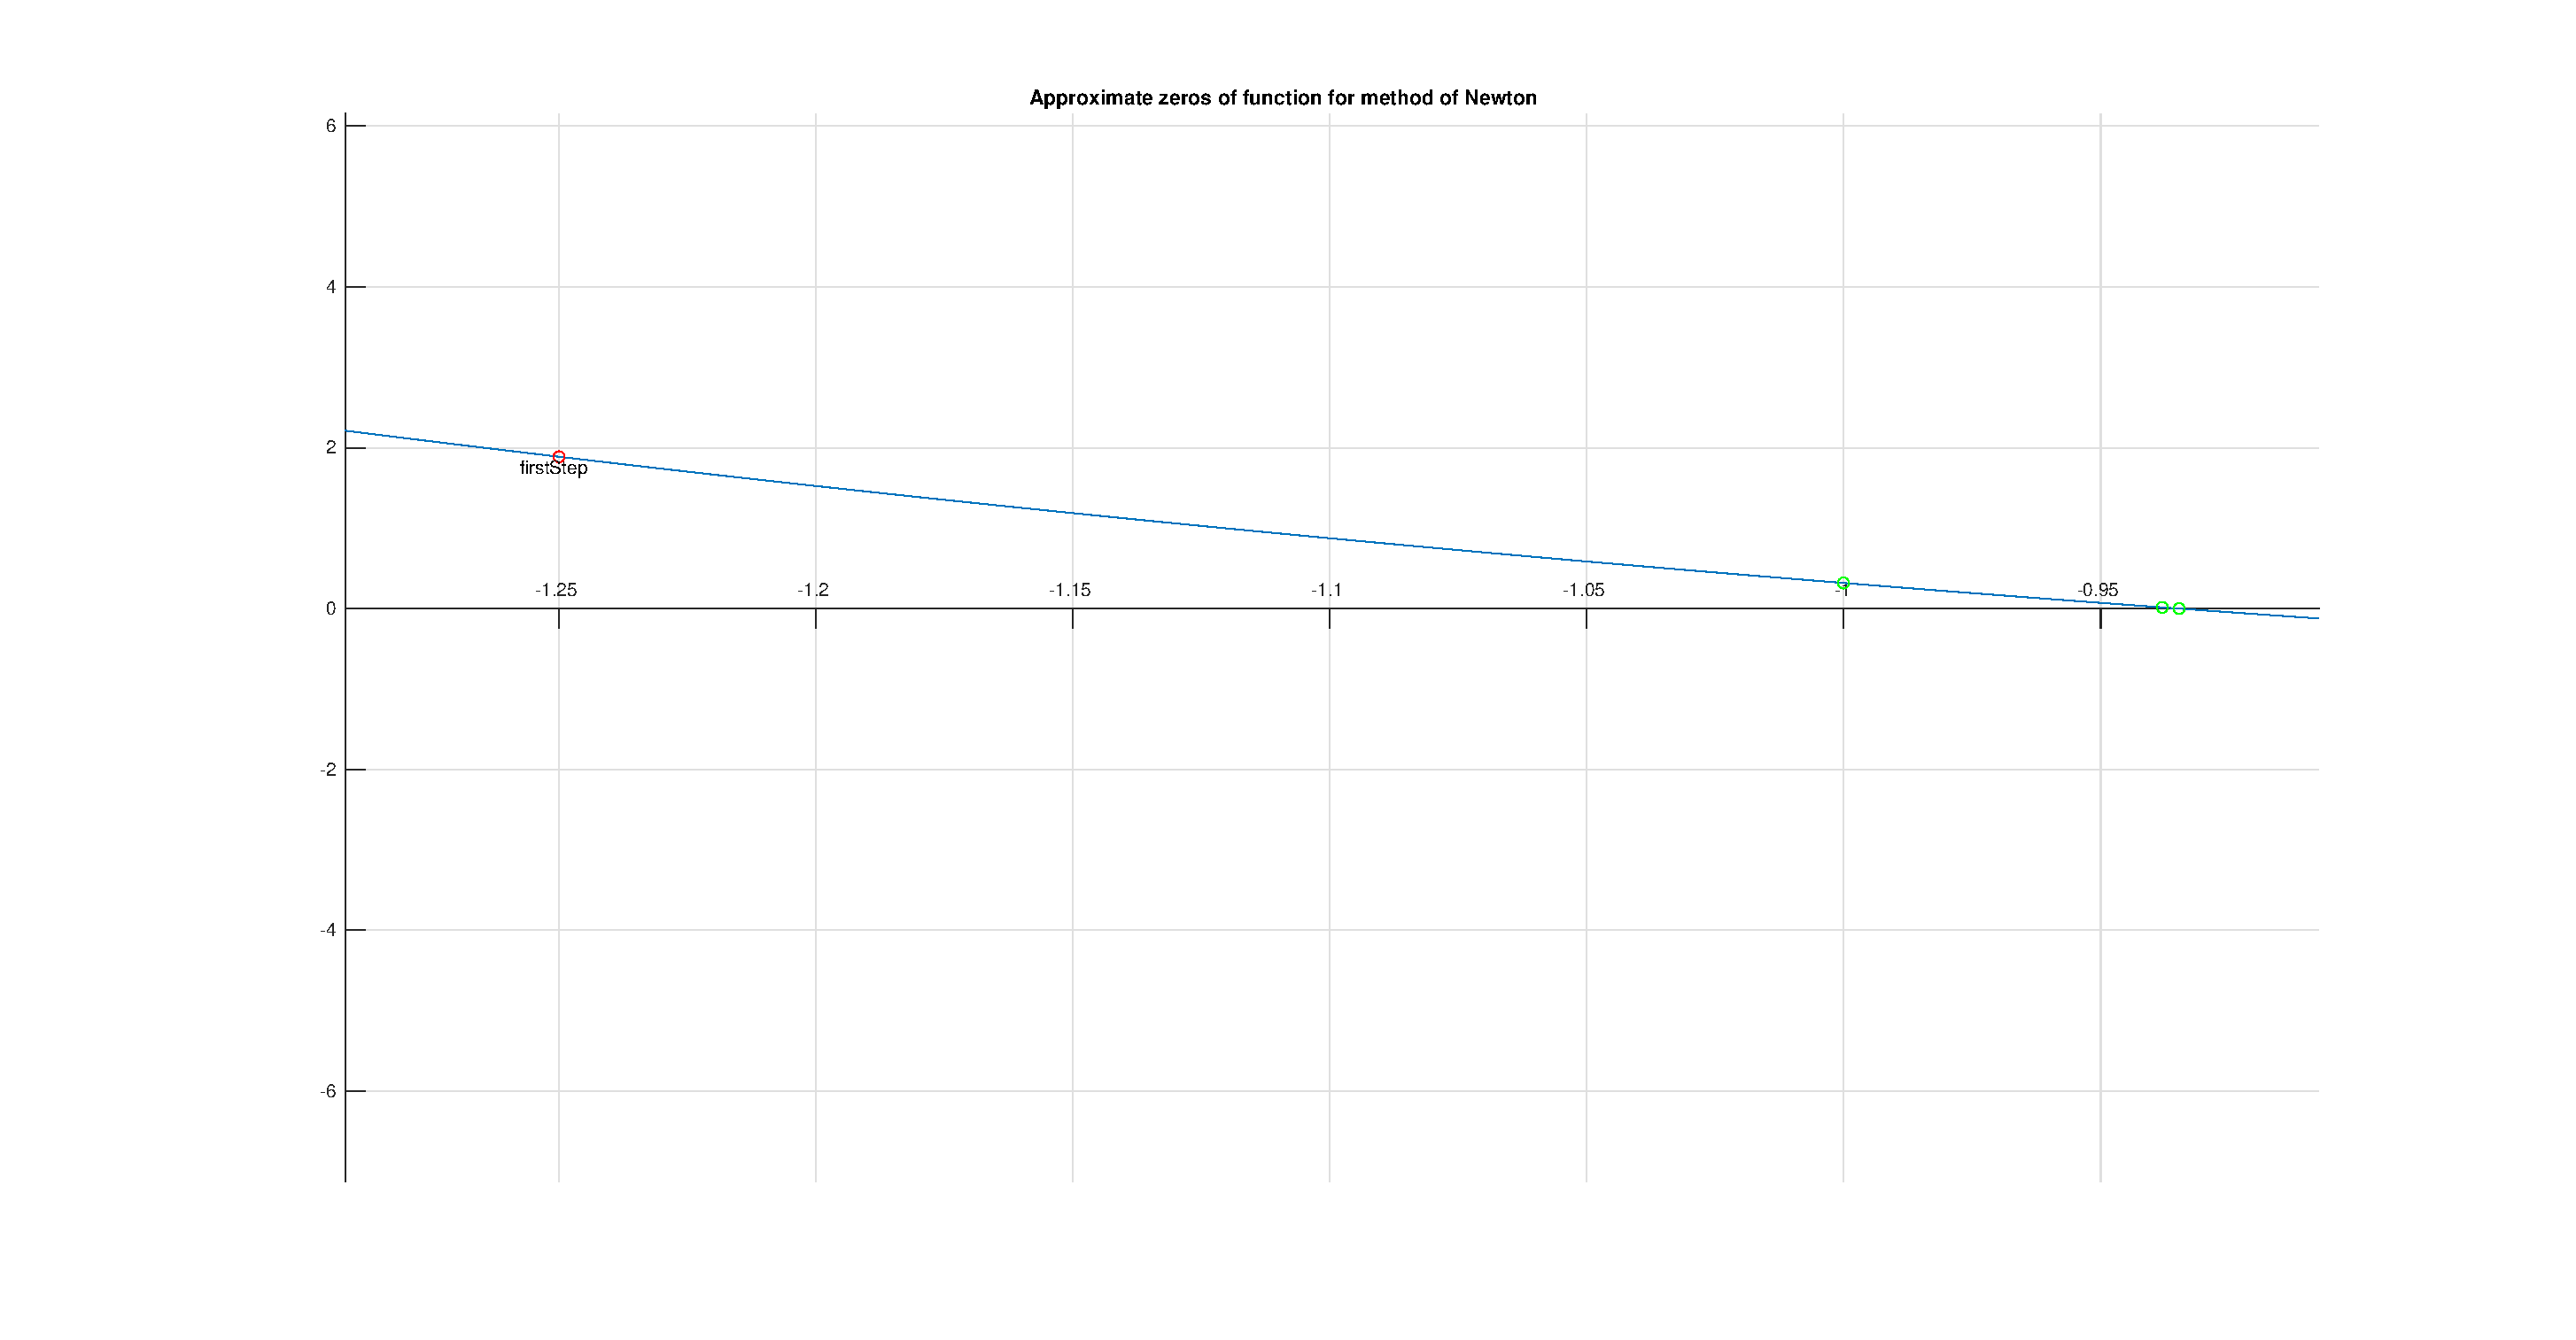
\includegraphics[scale=0.25]{task1Newtonzommedleft.eps}
\end{center}

\begin{center}
   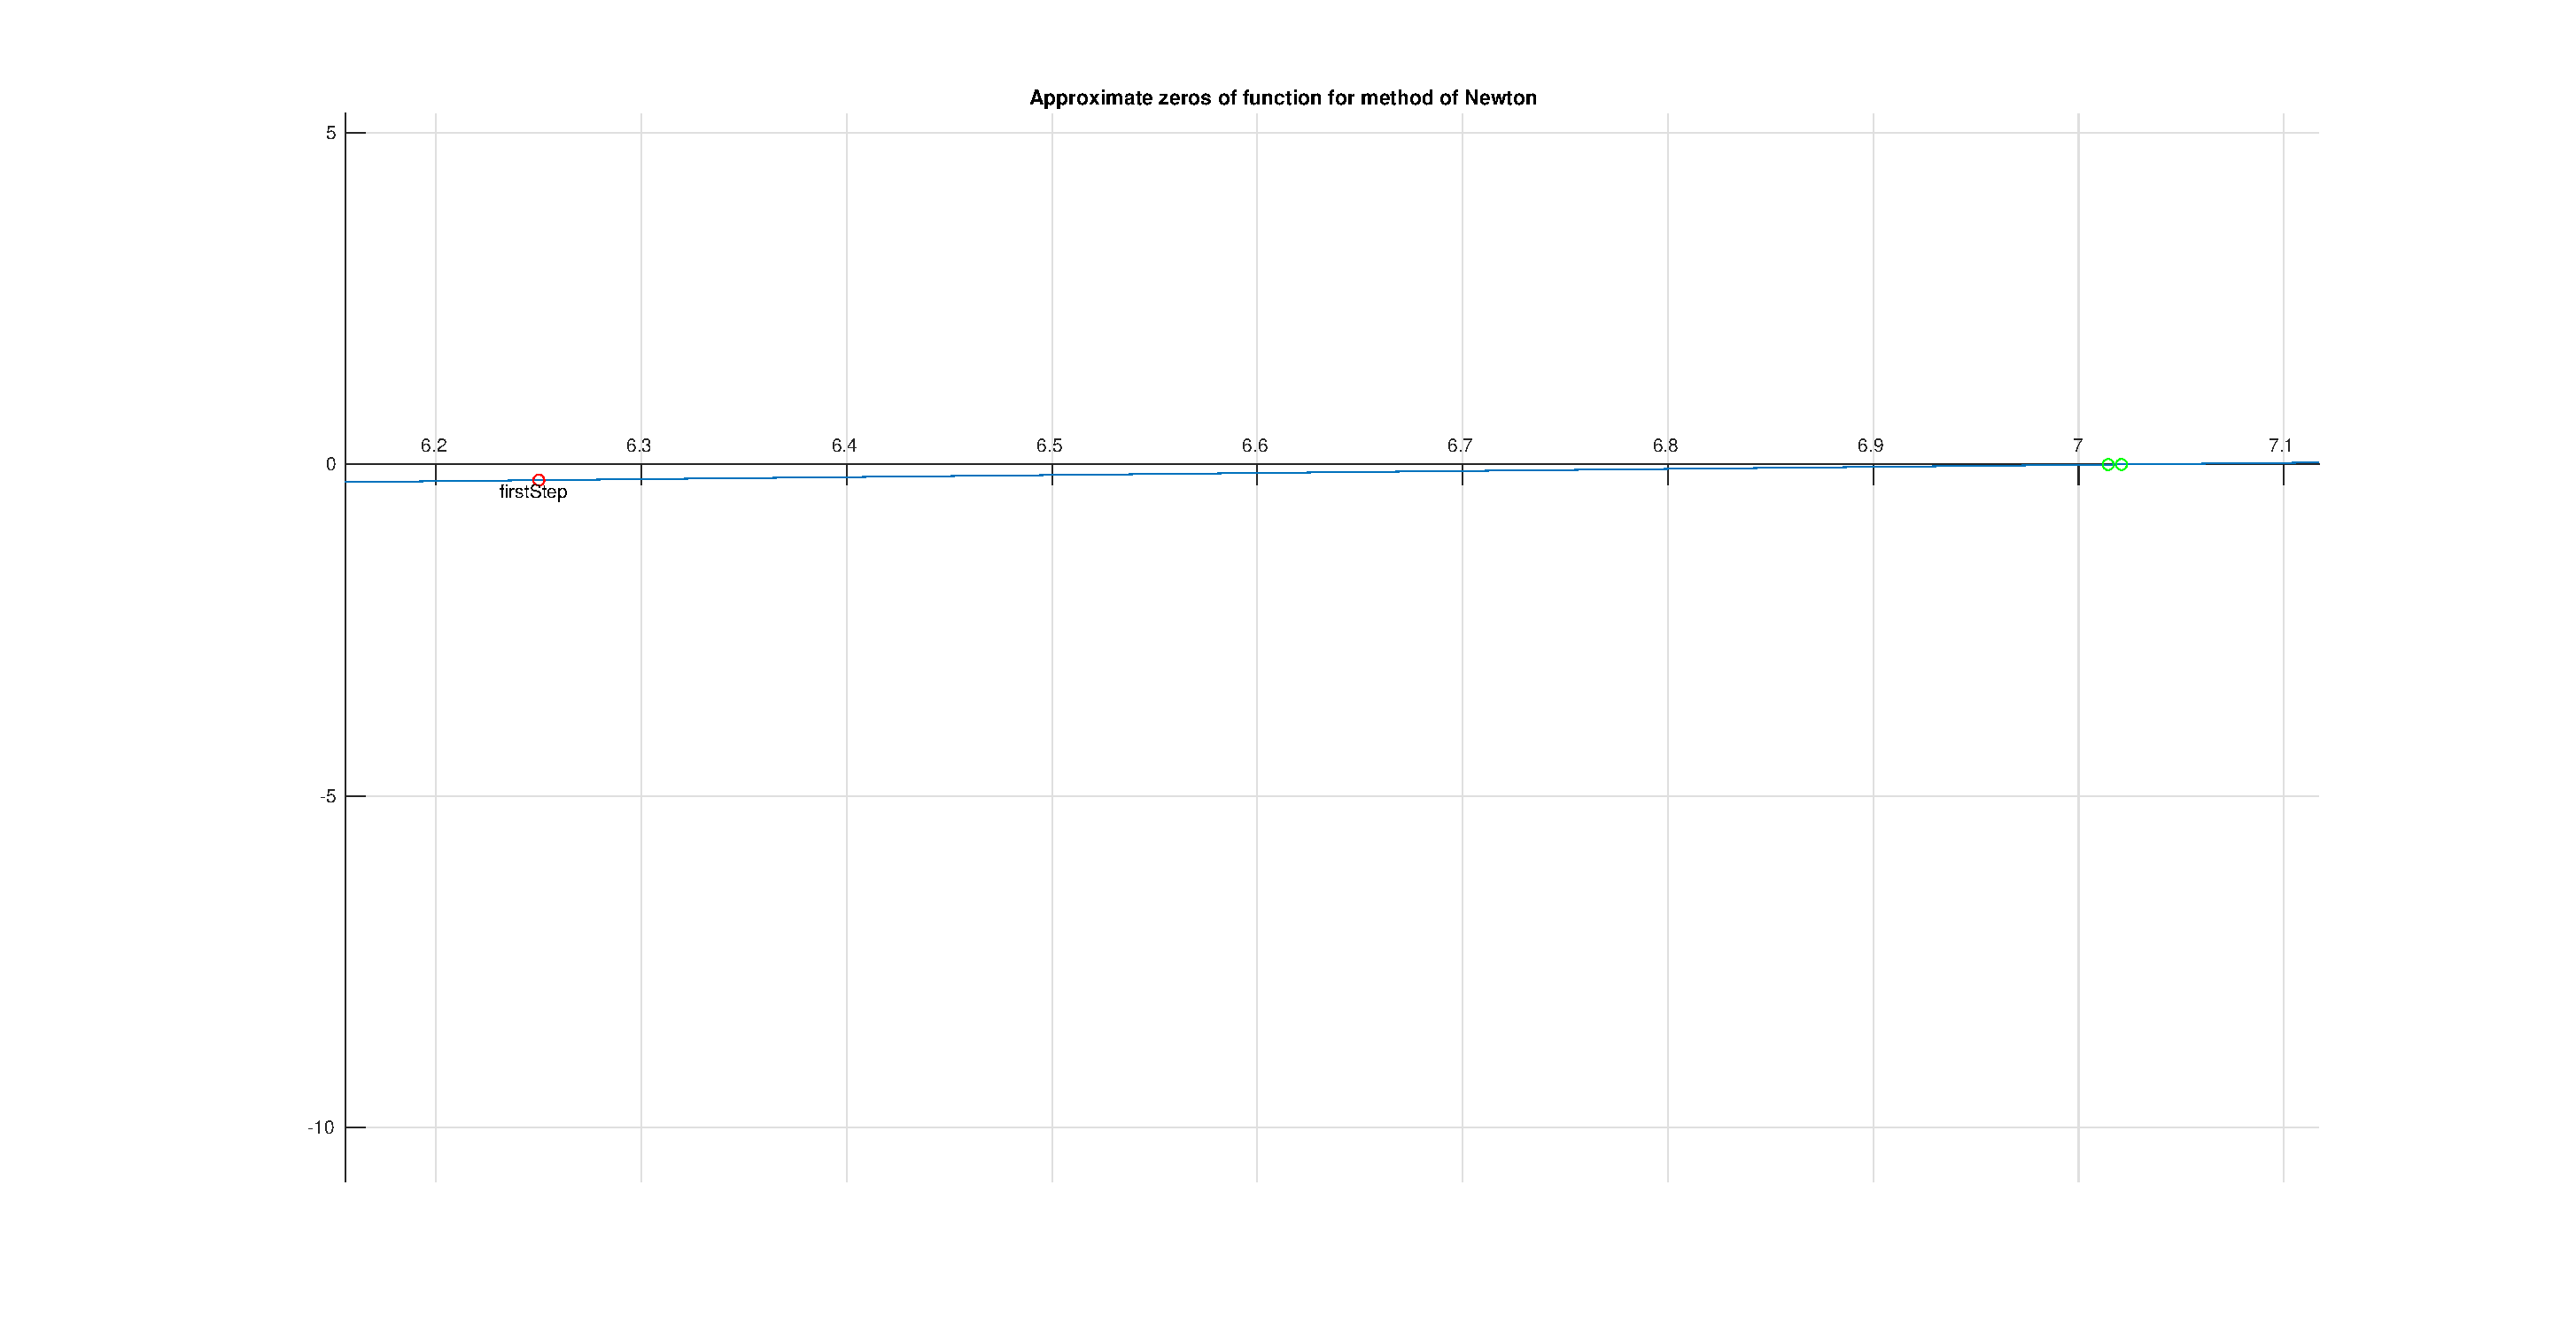
\includegraphics[scale=0.25]{task1Newtonzommedright.eps}
\end{center}

\begin{center}
  \begin{tabular}{| c  c c |}
\hline
Iteration & root         & f(root) \\
\hline
1   &      -1.25   &      1.8879  \\
\hline
2   &    -1.0001   &     0.31855  \\
\hline
3   &   -0.93804   &    0.015256  \\
\hline
4   &   -0.93476   &  4.0314e-05  \\
\hline
5   & -0.93475    & 2.8356e-10  \\
\hline
6   &   -0.93475   &           0  \\
\hline
\hline

\hline
\end{tabular}
\end{center}

\begin{center}
  \begin{tabular}{| c  c c |}
\hline
Iteration & root         & f(root) \\
\hline
1   &     6.25    &   -0.23707  \\
\hline
2    &  7.0144    & -0.0019866 \\
\hline
3     & 7.0209    & -9.517e-08  \\
\hline
4      &7.0209    &  7.468e-16  \\
\hline
\hline

\hline
\end{tabular}
\end{center}

\subsection{Discussion of results}
As we can see and as we could expect from theory Newton method reigns supreme.
It is:
\begin{enumerate}
\item Faster.
Especially for finding first root. It took 36 iterations for false position method to find first root with accuary up to $10^{-10}$ and it took only 6 iterations for the Newton method.
\item More accurate
Not only that we also got more accurate results with Newton method! With first root being so close to the real answer that the matlab calculated the value of this function at this point as exactly equal to 0. For second root the accuary is $10^{6}$ better than for the false position method.
\item Smaller gaps
Looking at graphs we got from both method we can clearly see that the gaps between the final result and each and every step are much smaller for Newton method. This again proves that it is faster and more accurate compared to false position method.
\end{enumerate}



\chapter{Find real and complex roots of the polynomial}

\section{Problem}

We have to find all real and complex roots of the polynomial:

\[ f(x) = a_4x^4+a_3x^3+a_2x^2+a_1x+a_0 \]
where:
\[ [a_4 \; a_3 \; a_2 \; a_1 \; a_0] = [-2 \; 12 \; 4 \; 1 \; 3] \]

So our polynomial looks like this:
\[ f(x) = -2x^4+12x^3+4x^2+1x+3 \]

Using the M{\"u}ller's method. We have to implement both MM1 and MM2 versions. We also need to find real roots using the Newton's method and compare these results with what we got from MM2 version of the M{\"u}ller's method.
\section{Theoretical Introduction}
M{\"u}ller's method revoles around the idea of approximating the polynomial locally close to the root by a quadratic function. Based on three different points we can use quadratic interpolation and develop our method. This means that we can treat it as a generalization of secant method. That being said we can also realize it in an efficient way if we use just one point. We can use for this case values of polynomial, and its first and second derrivative at current point.

Accordingly there are two versions of M{\"u}ller's method: \textbf{MM1} and \textbf{MM2}.

\subsection{MM1}
Given three points: $x_0; x_1; x_2$ and their polynomial values: $f(x_0), f(x_1), f(x_2)$ we construct a (quadratic) function passing through these points. Then we find roots of this parabola and we choose one of these rots for the approximation of the result.

For example:
Assume that $x_2$ is the approximation of the root.
Let's introduce variable $z$ such that:
\[ z = x - x_2 \]
And differences:
\[ z_0 = x_0 - x_2 \]
\[ z_1 = x_1 - x_2 \]

We have quadratic function:
\[ y(z) = az^2 + bz + c \]

Using three points from above we get:
\[ y(z_0) = az_0^2 + bz_0 + c = f(x_0) \]
\[ y(z_1) = az_1^2 + bz_1 + c = f(x_1) \]
\[ y(z_2) = c = f(x_2) \]

And then we get system of equation that we can solve to find $a$ and $b$:
\[ az_0^2 + bz_0 = f(x_0) - f(x_2) \]
\[ az_1^2 + bz_1 = f(x_1) - f(x_2) \]

Roots are equal to:
\[ z_+ = \frac{-2c}{b+\sqrt{b^2 - 4ac}} \]
\[ z_- = \frac{-2c}{b-\sqrt{b^2 - 4ac}} \]

We choose a root with smaller absolute value for next iteration:
\[ z_{min} = \min{|z_+, z_-|} \]
\[ x_3 = x_2 + z_{min} \]

Then we choose new point $x_3$ and two selected from $x_0, x_1, x_2$ which were closer to $x_3$.

This method should also work for $\Delta < 0 $


\subsection{MM2}
This method being numerically more effective is usually recommended.
We calculate values of a polynomial and its first and second derrivatives at one point.

from definition of quadratic function:
\[ y(z) = az^2 + bz + c \]
we can get:
\[ z = x - x_k \]
If $z = 0$ then:
\[ y(0) = c = f(x_k) \]
\[ y^{'}(0) = b = f^{'}(x_k) \]
\[ y^{''}(0) = 2a = f^{''}(x_k) \]

We can derive from that formula for roots:

\[ z_{\pm} = \frac{-2f(x_k)}{f^{'}(x_k) \pm \sqrt{ (f^{'}(x_k))^2 - 2f(x_k)f^{''}(x_k)}}\]

Then we choose root with smaller absolute value for next iteration:
\[ x_{k+1} = x_k + z_{min} \]

Again this method should be implemented in complex number arithmetic.
This method is locally convergent with order of convergence equal to 1.84. It is locally more effective that secant method and it is almost as fast as Newton's method while being capable of finding complex roots. It can be used to find roots of polynomials or another nonlinear functions.

\section{Results}

\subsection{Graphs for MM1}
\begin{center}
   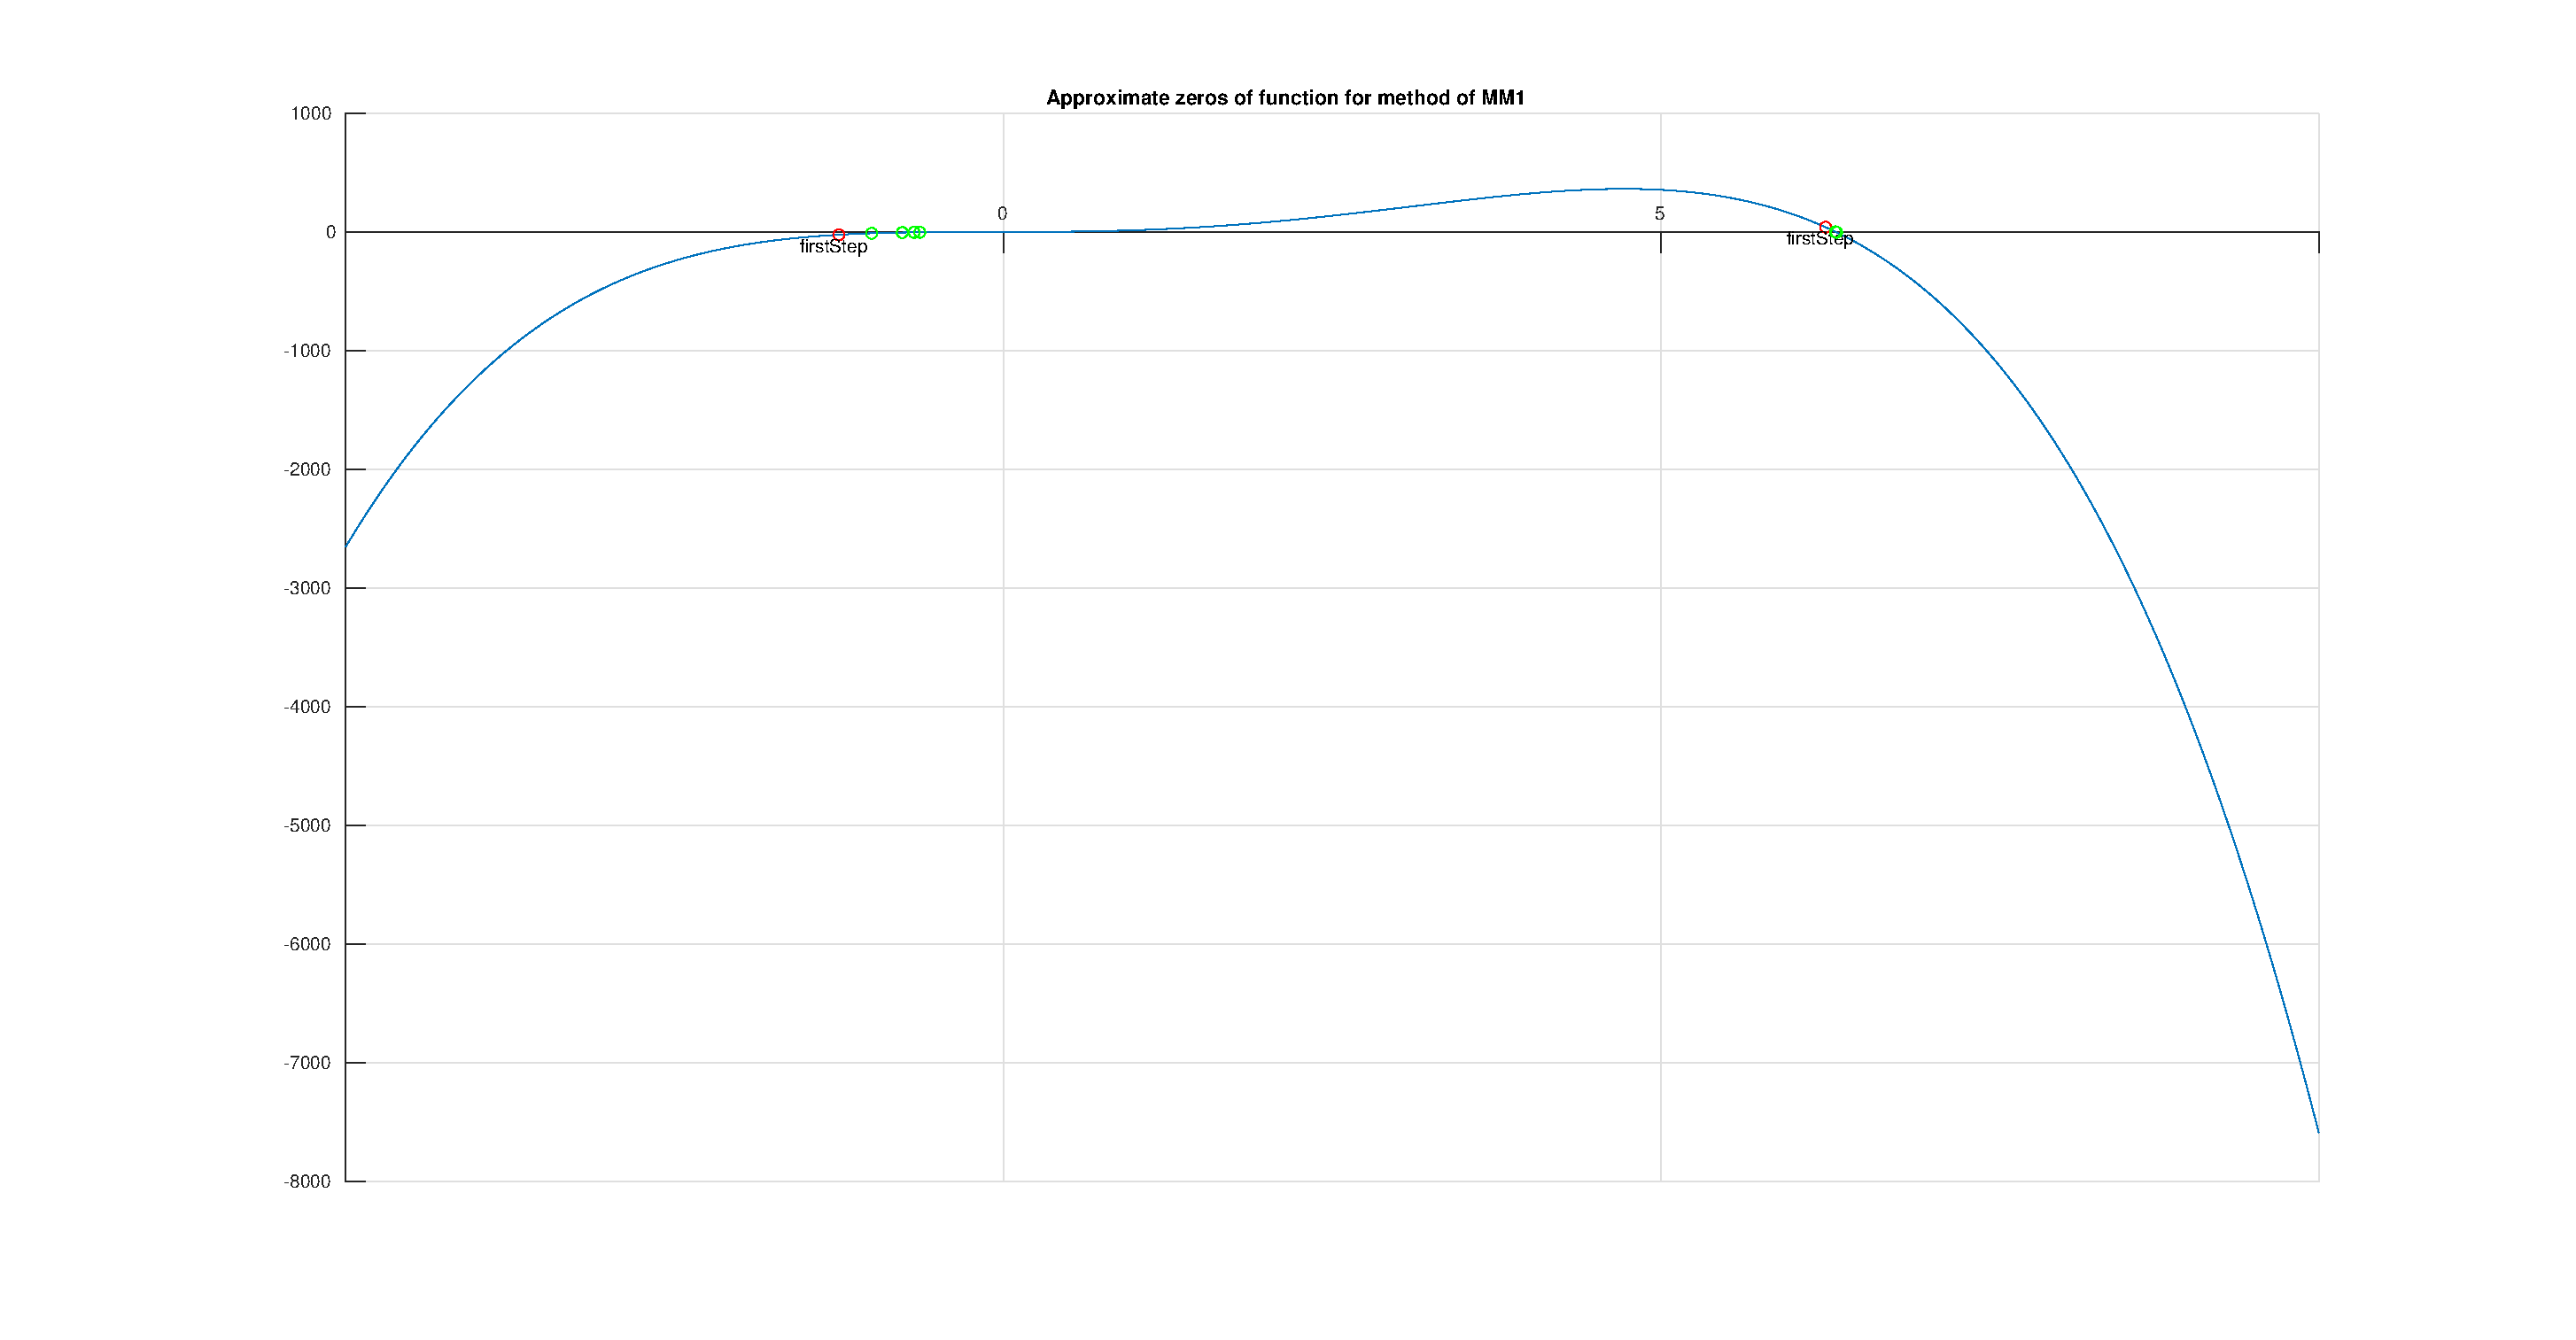
\includegraphics[scale=0.25]{task2mm1realoverall.eps}
\end{center}

\begin{center}
   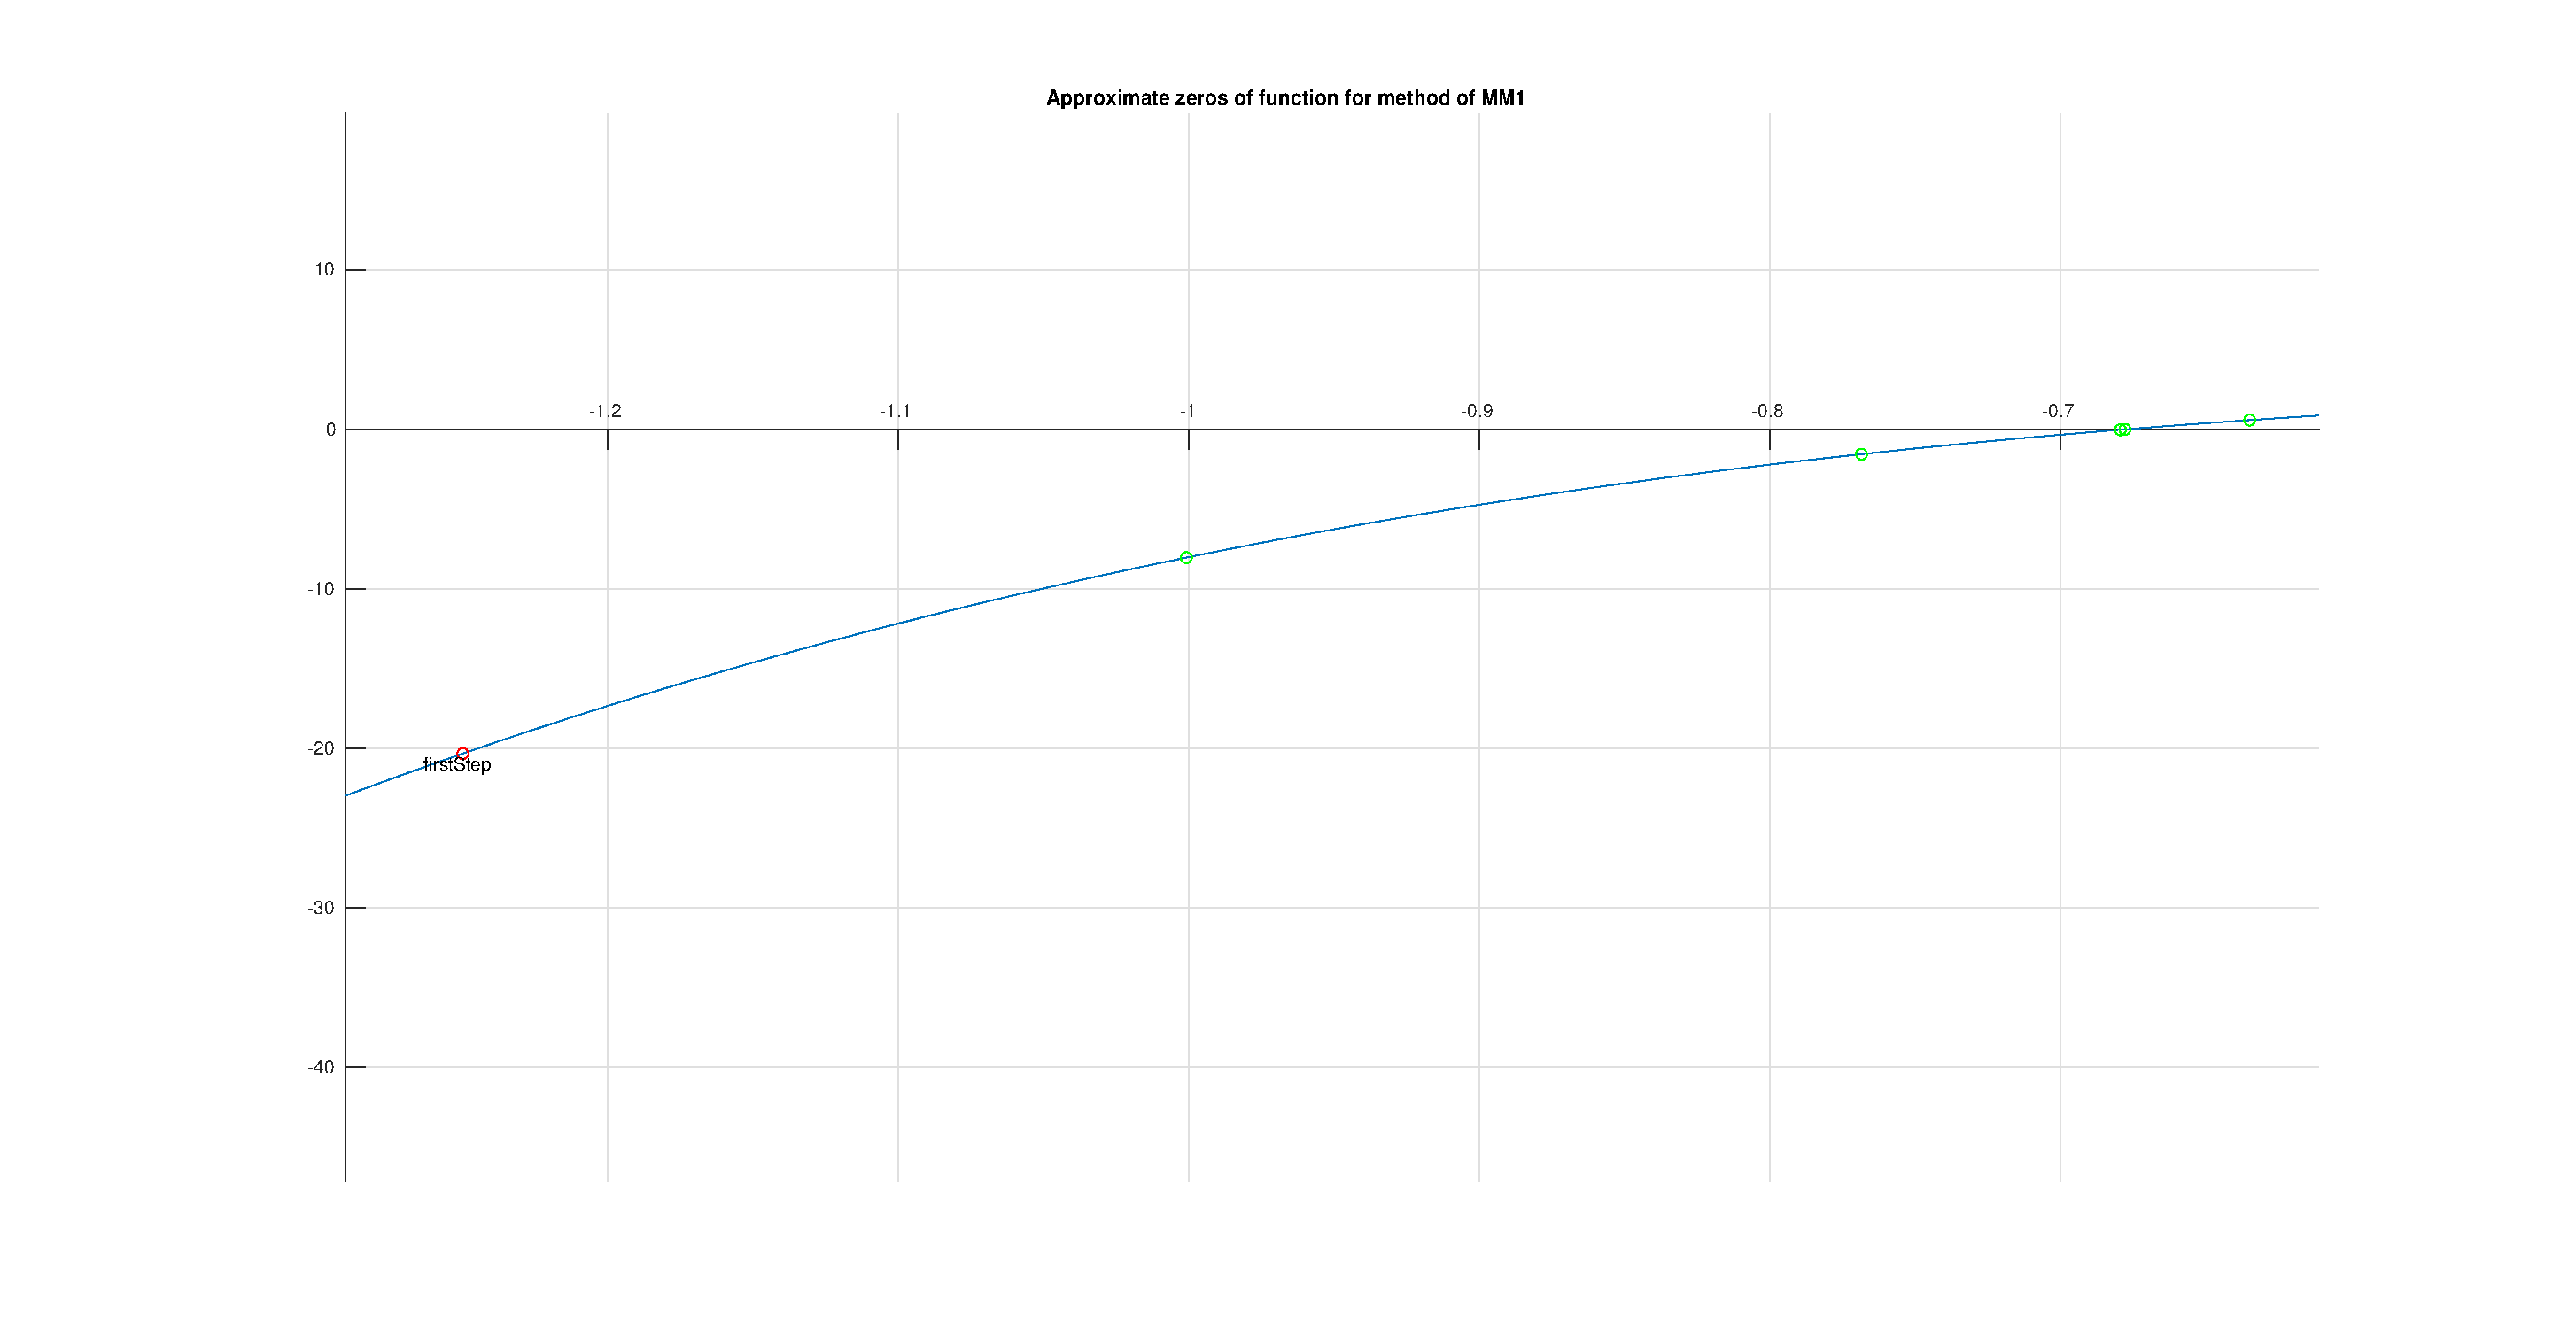
\includegraphics[scale=0.25]{task2mm1realleft.eps}
\end{center}

\begin{center}
   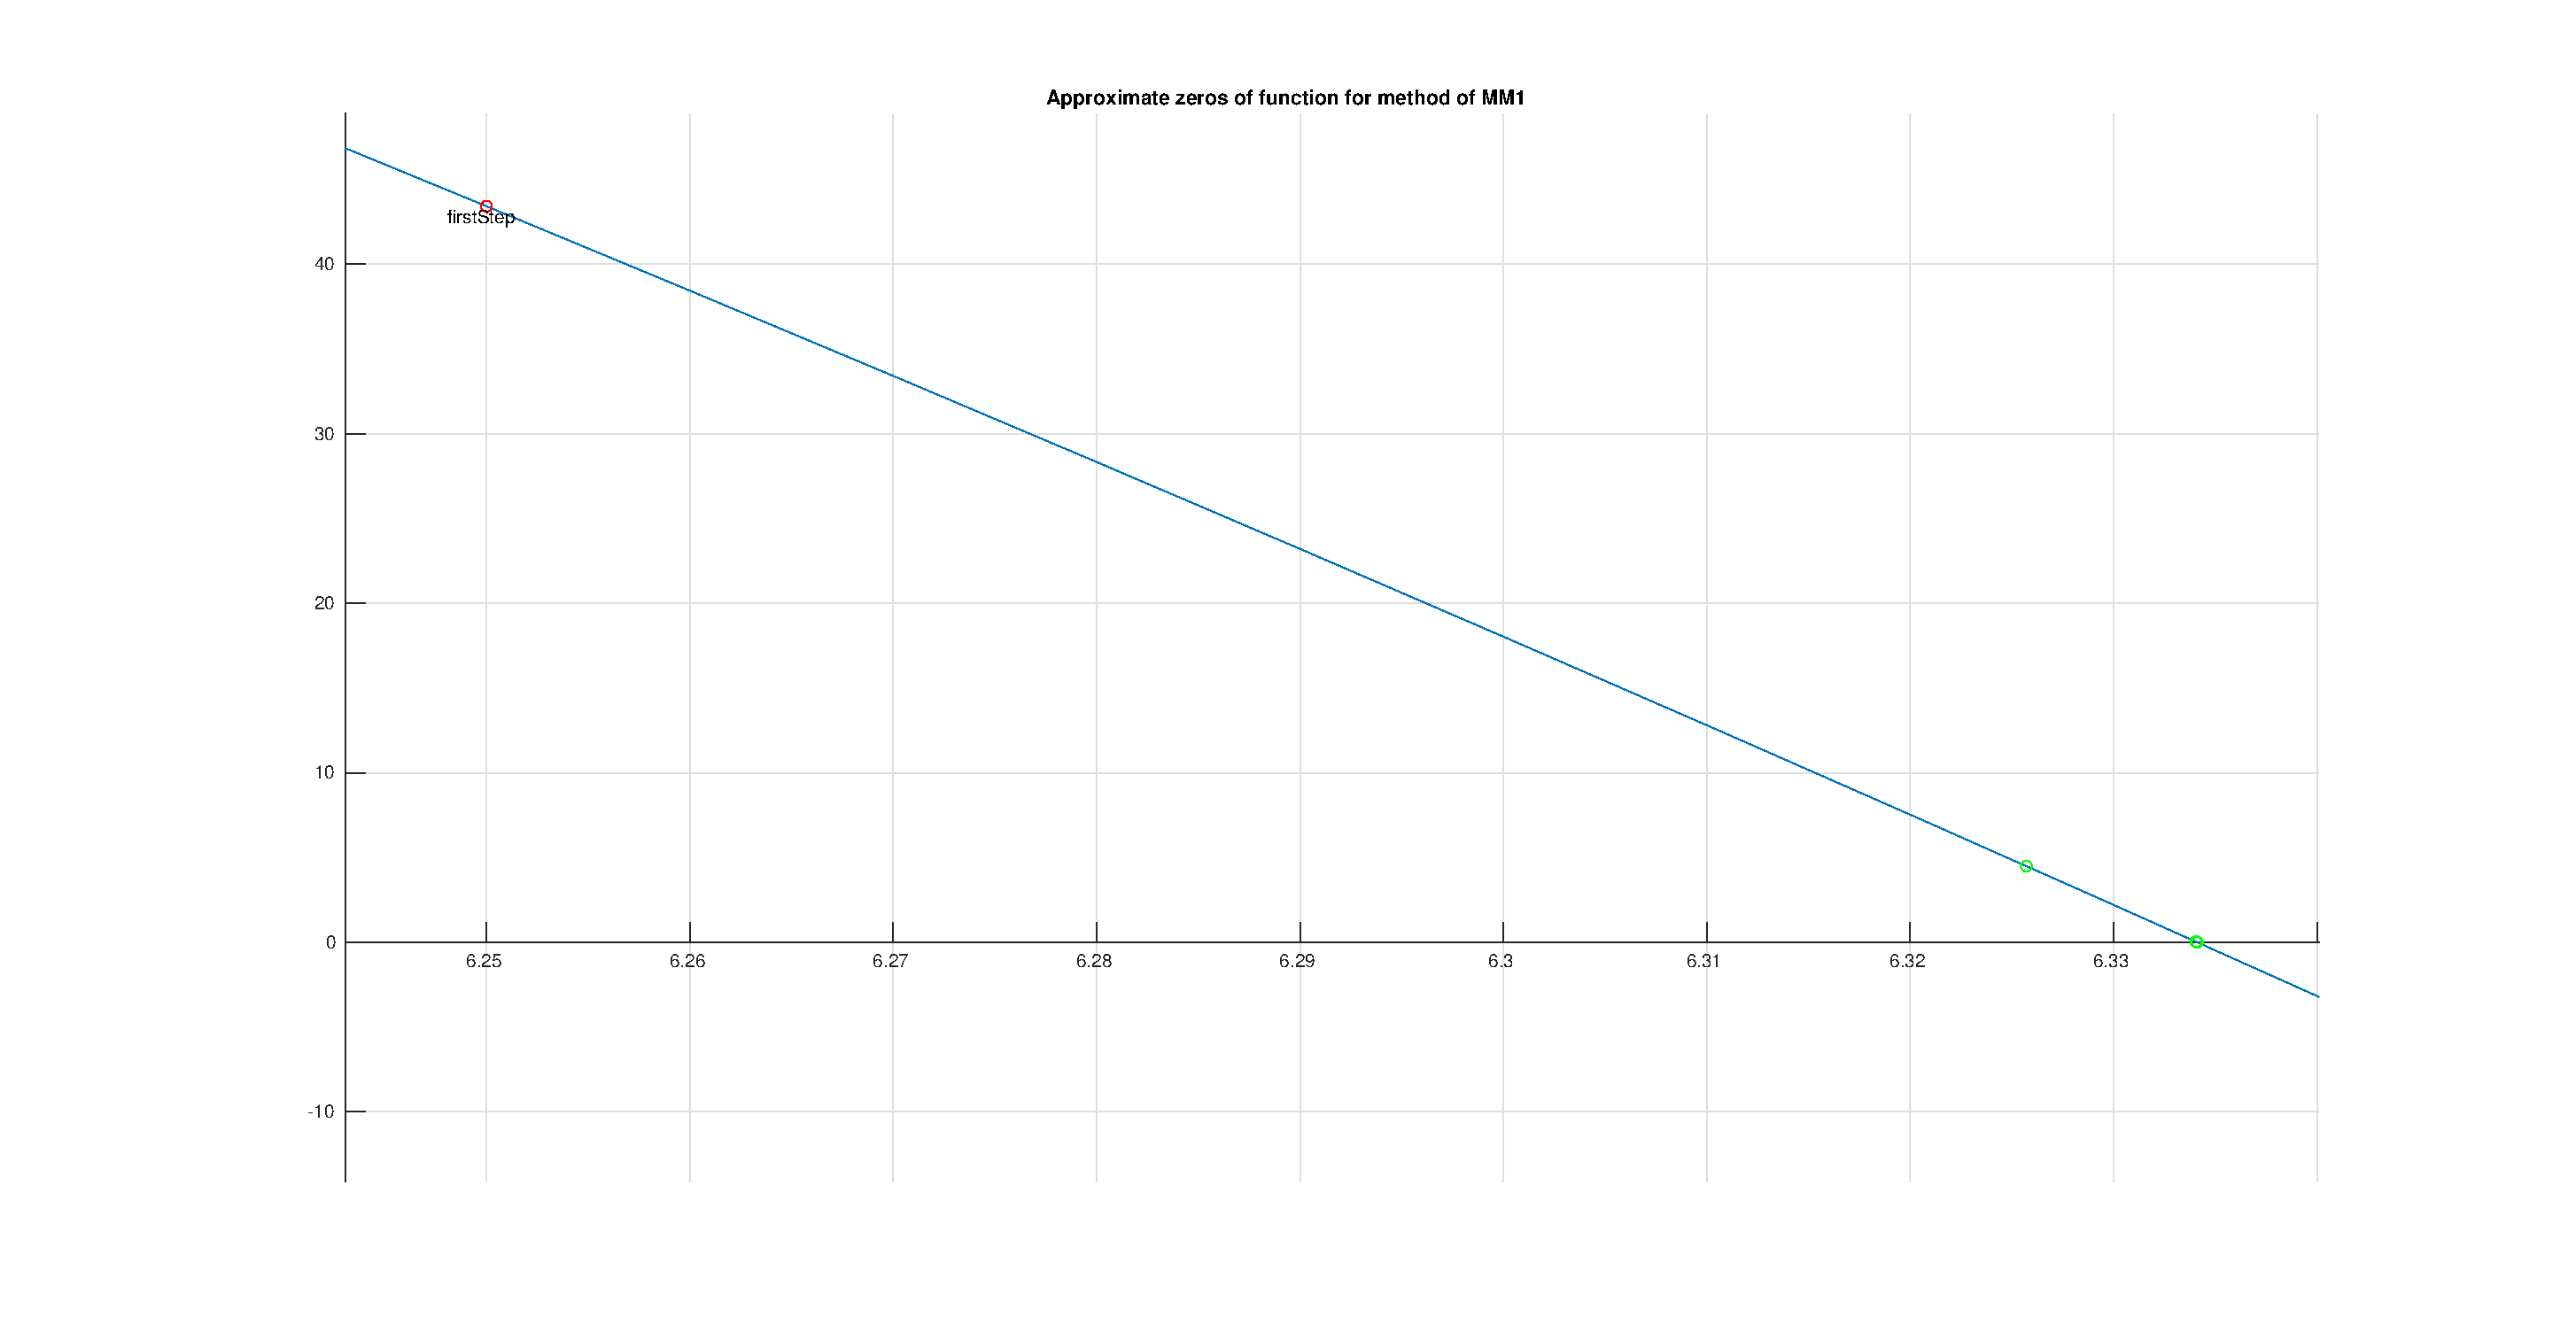
\includegraphics[scale=0.25]{task2mm1realright.eps}
\end{center}

\begin{center}
   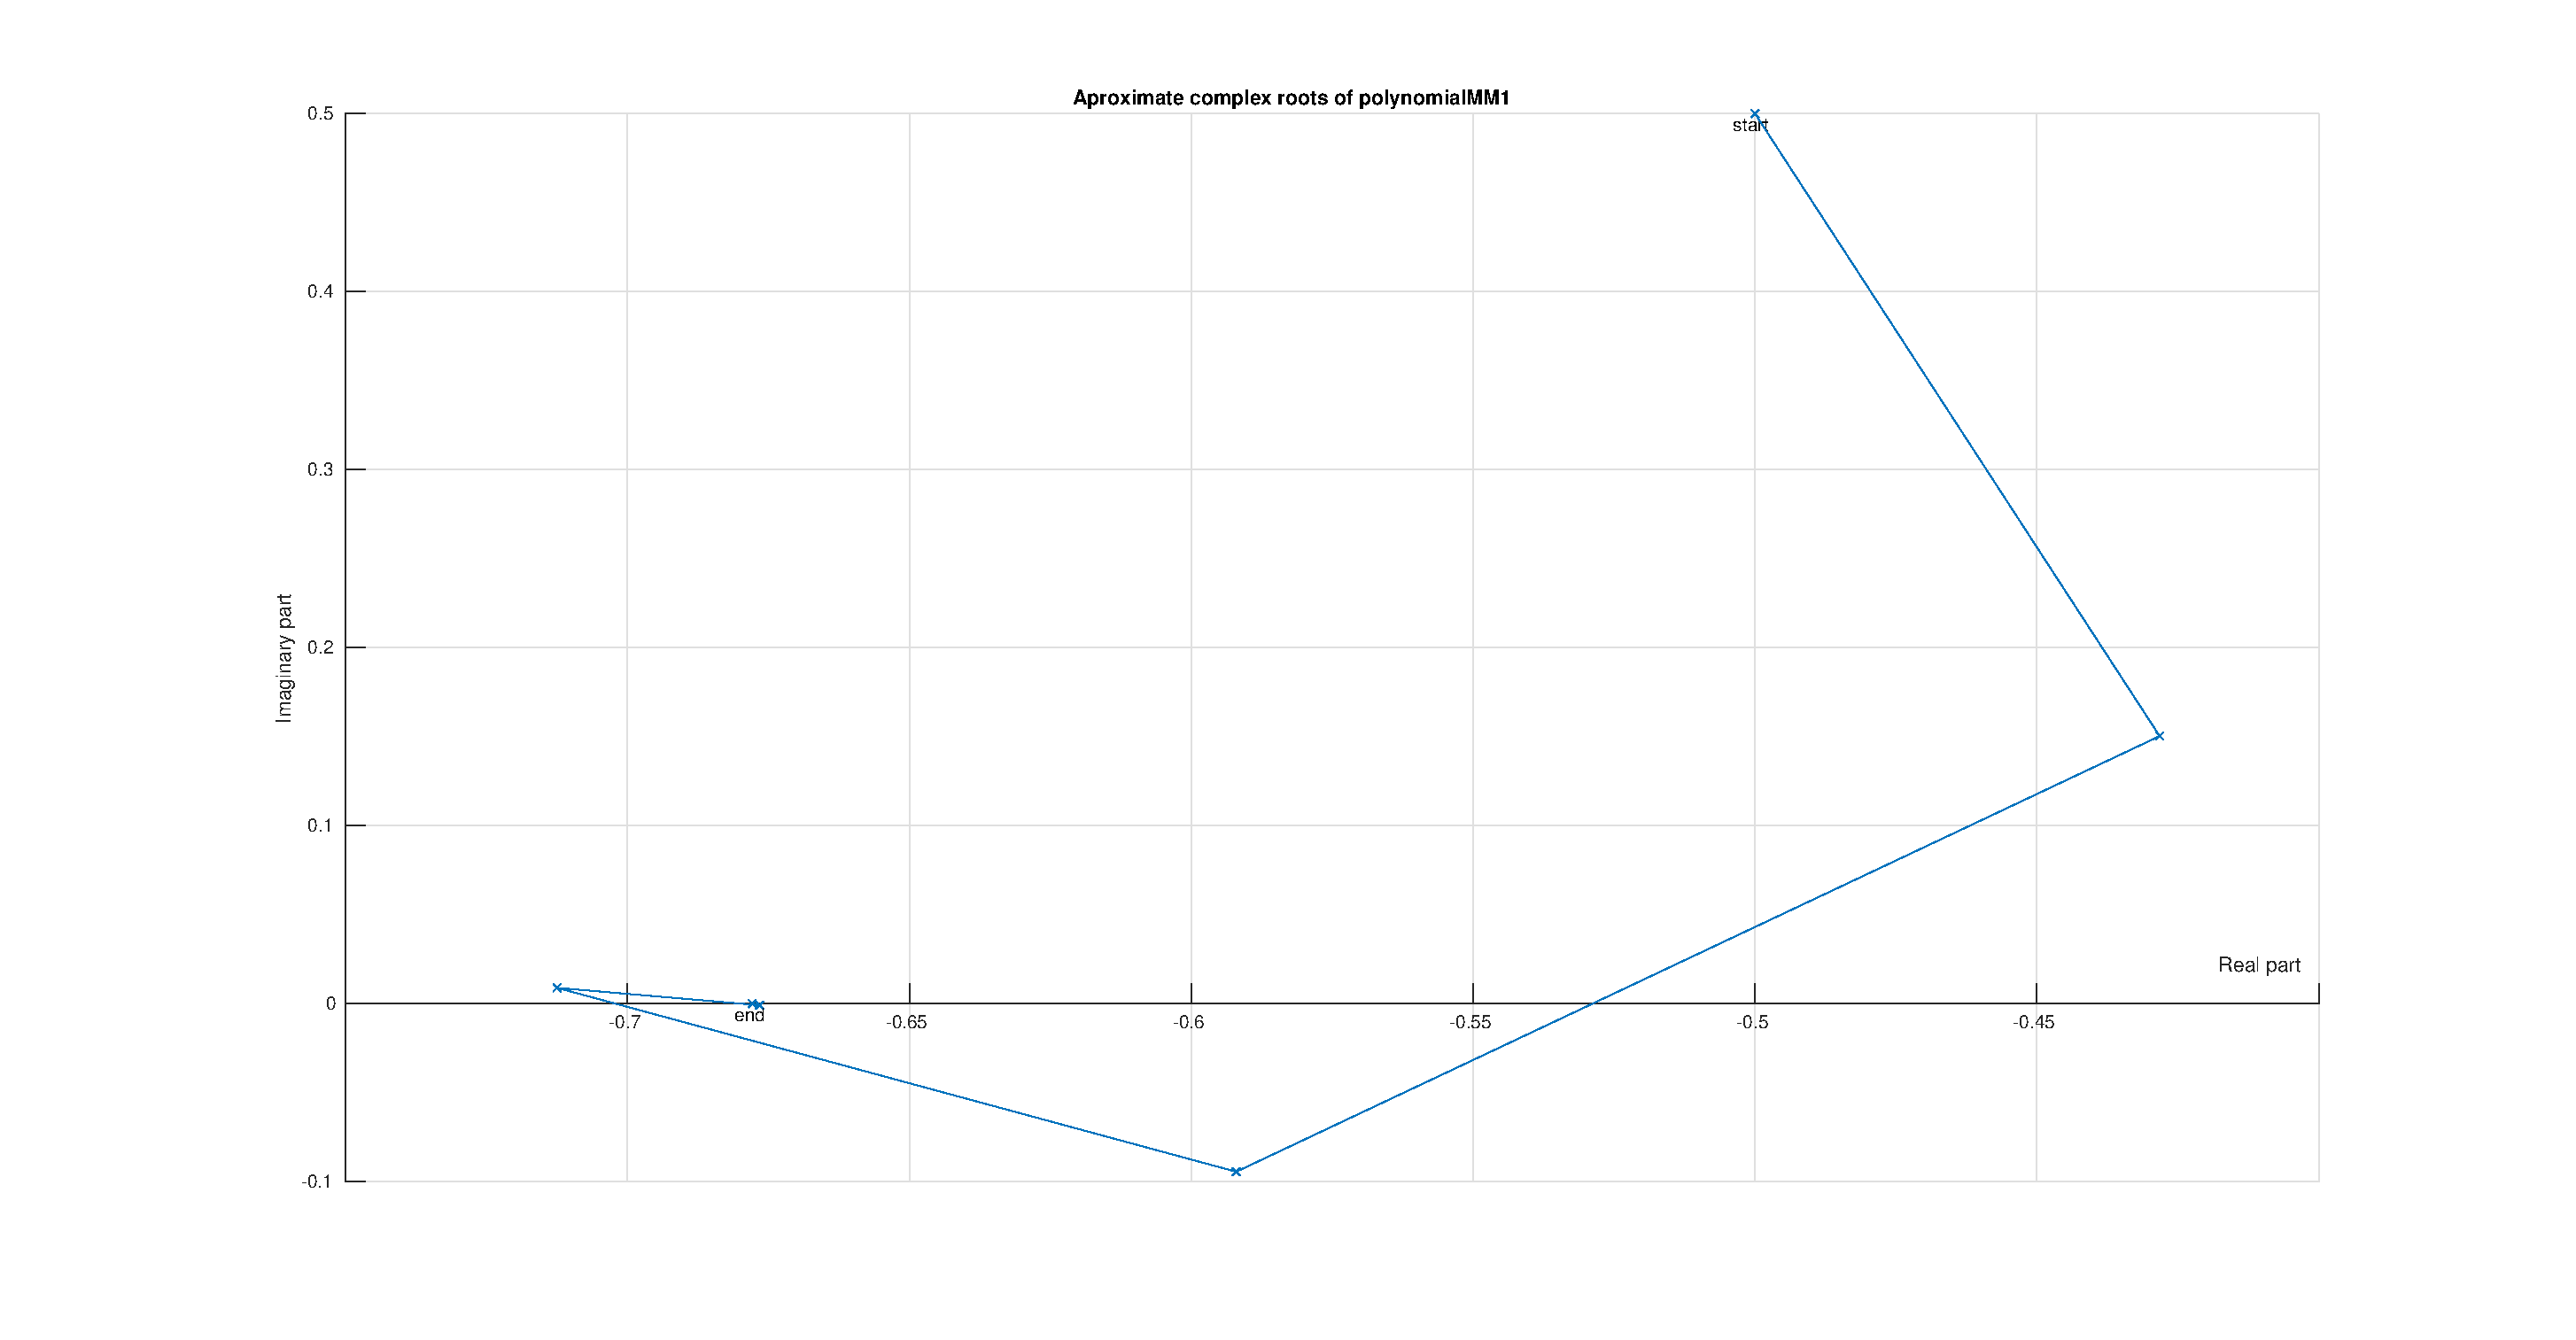
\includegraphics[scale=0.25]{task2mm1complexoverall.eps}
\end{center}

\begin{center}
   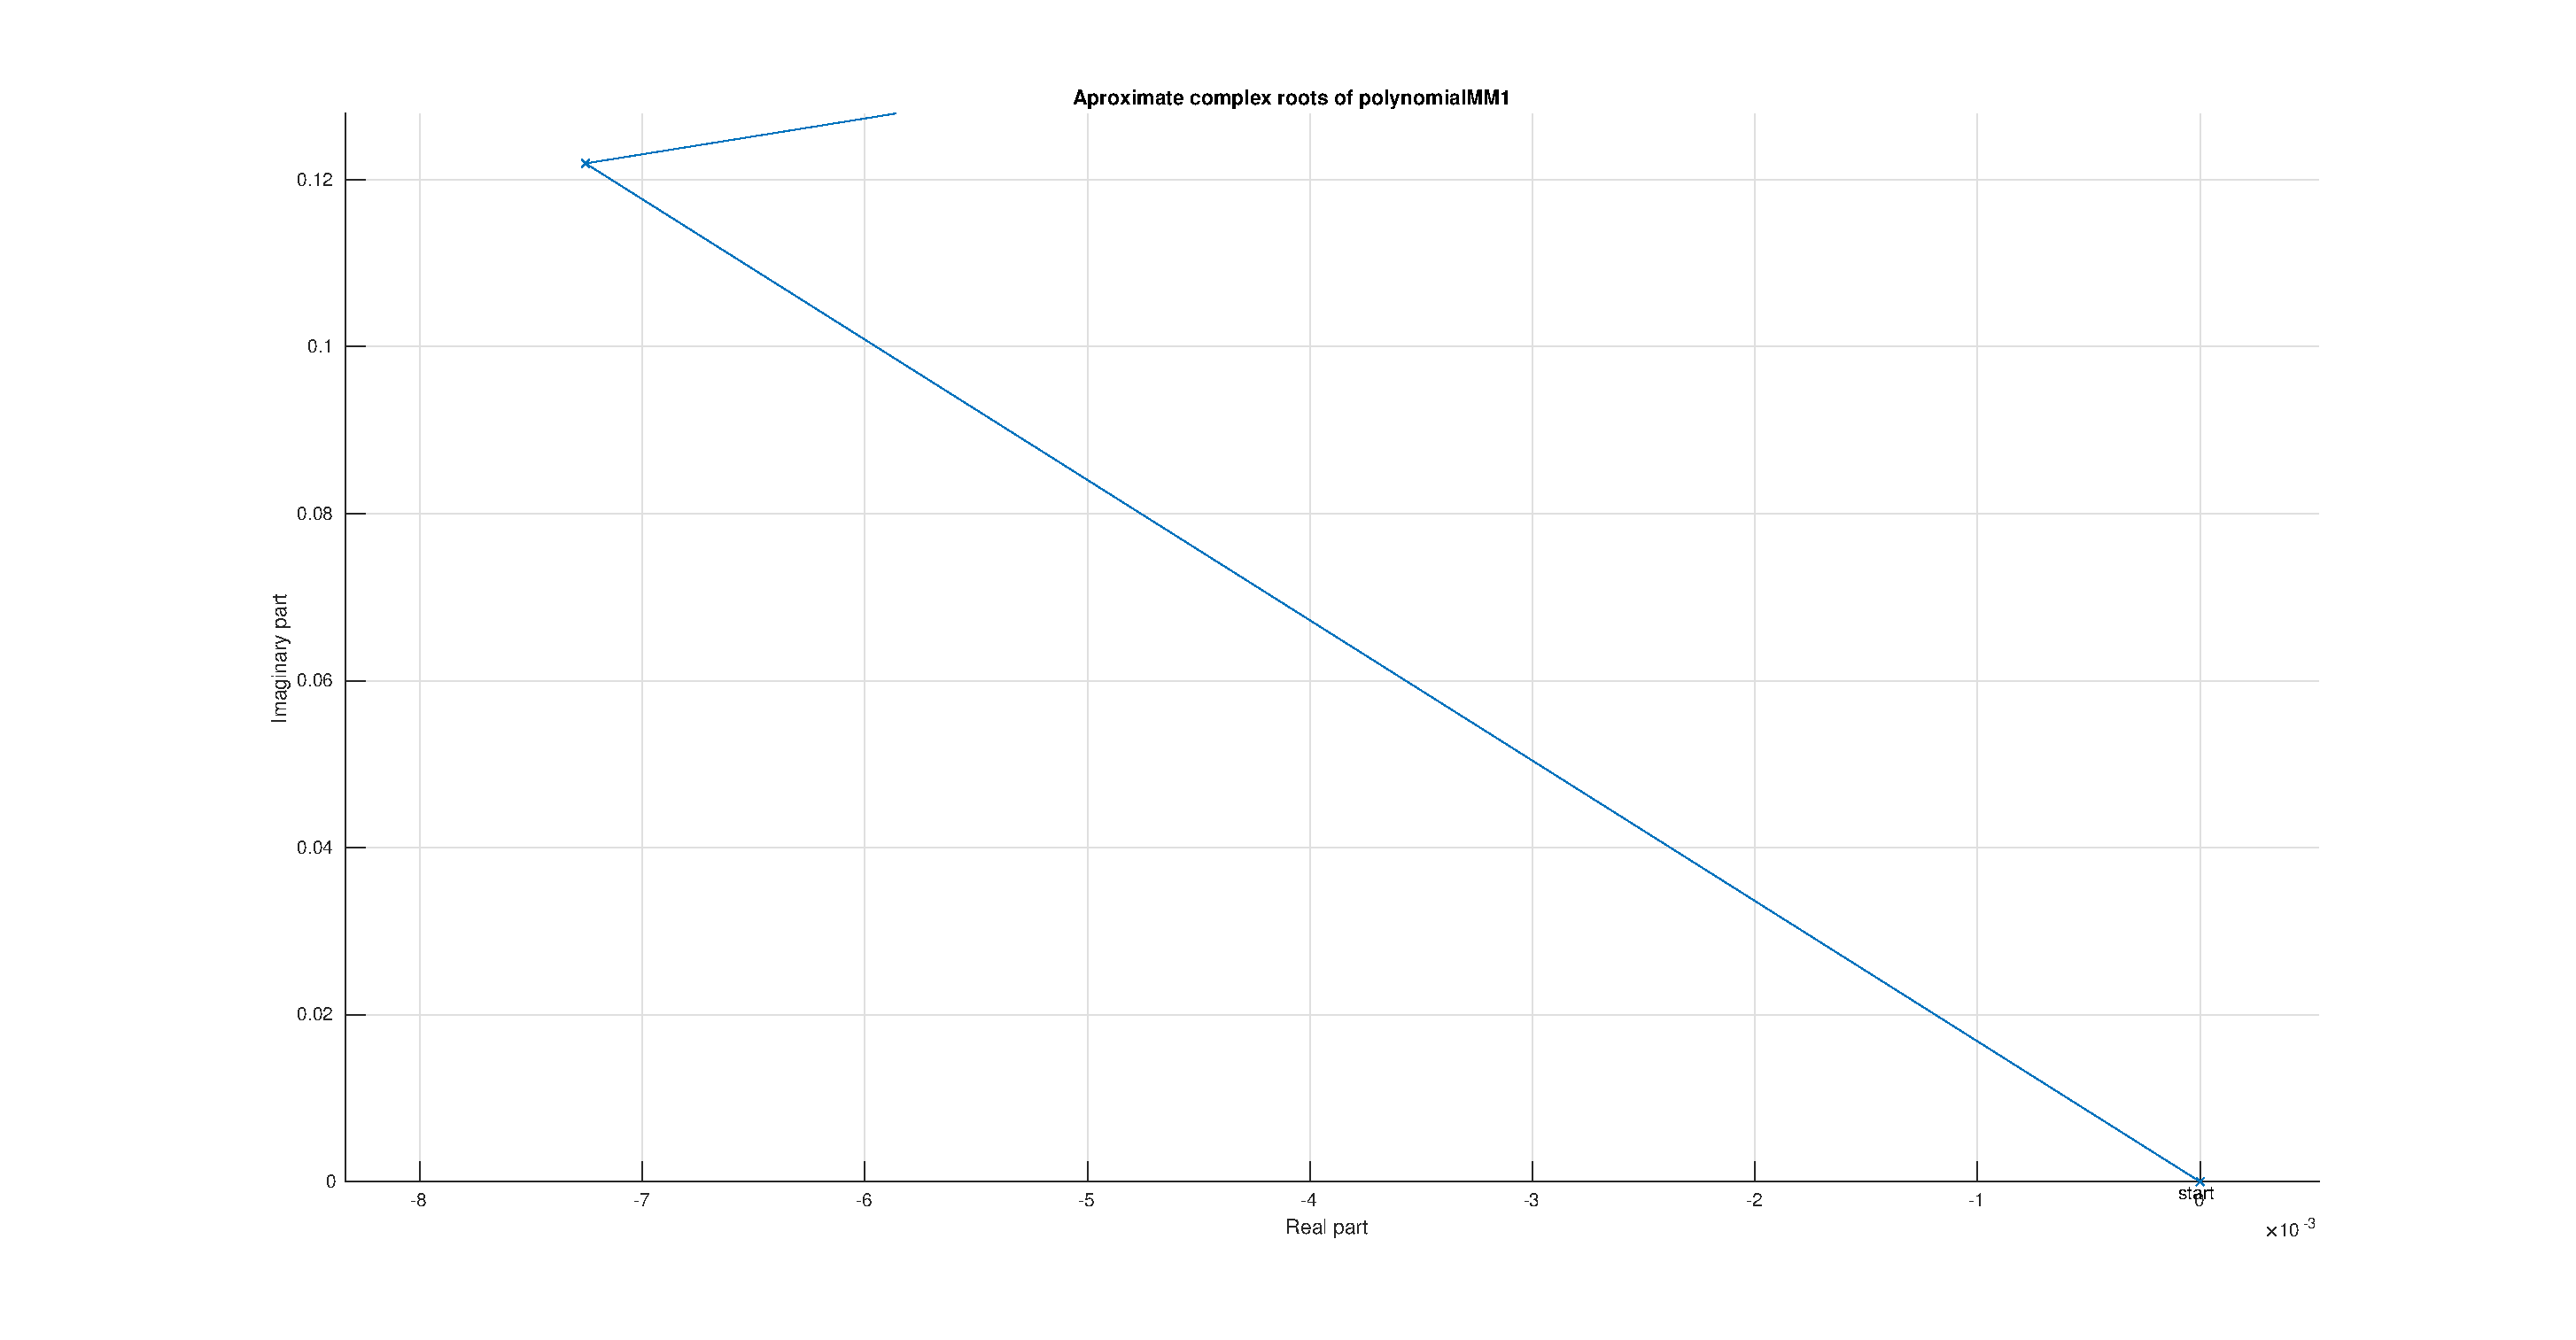
\includegraphics[scale=0.25]{task2mm1complexdown.eps}
\end{center}

\begin{center}
   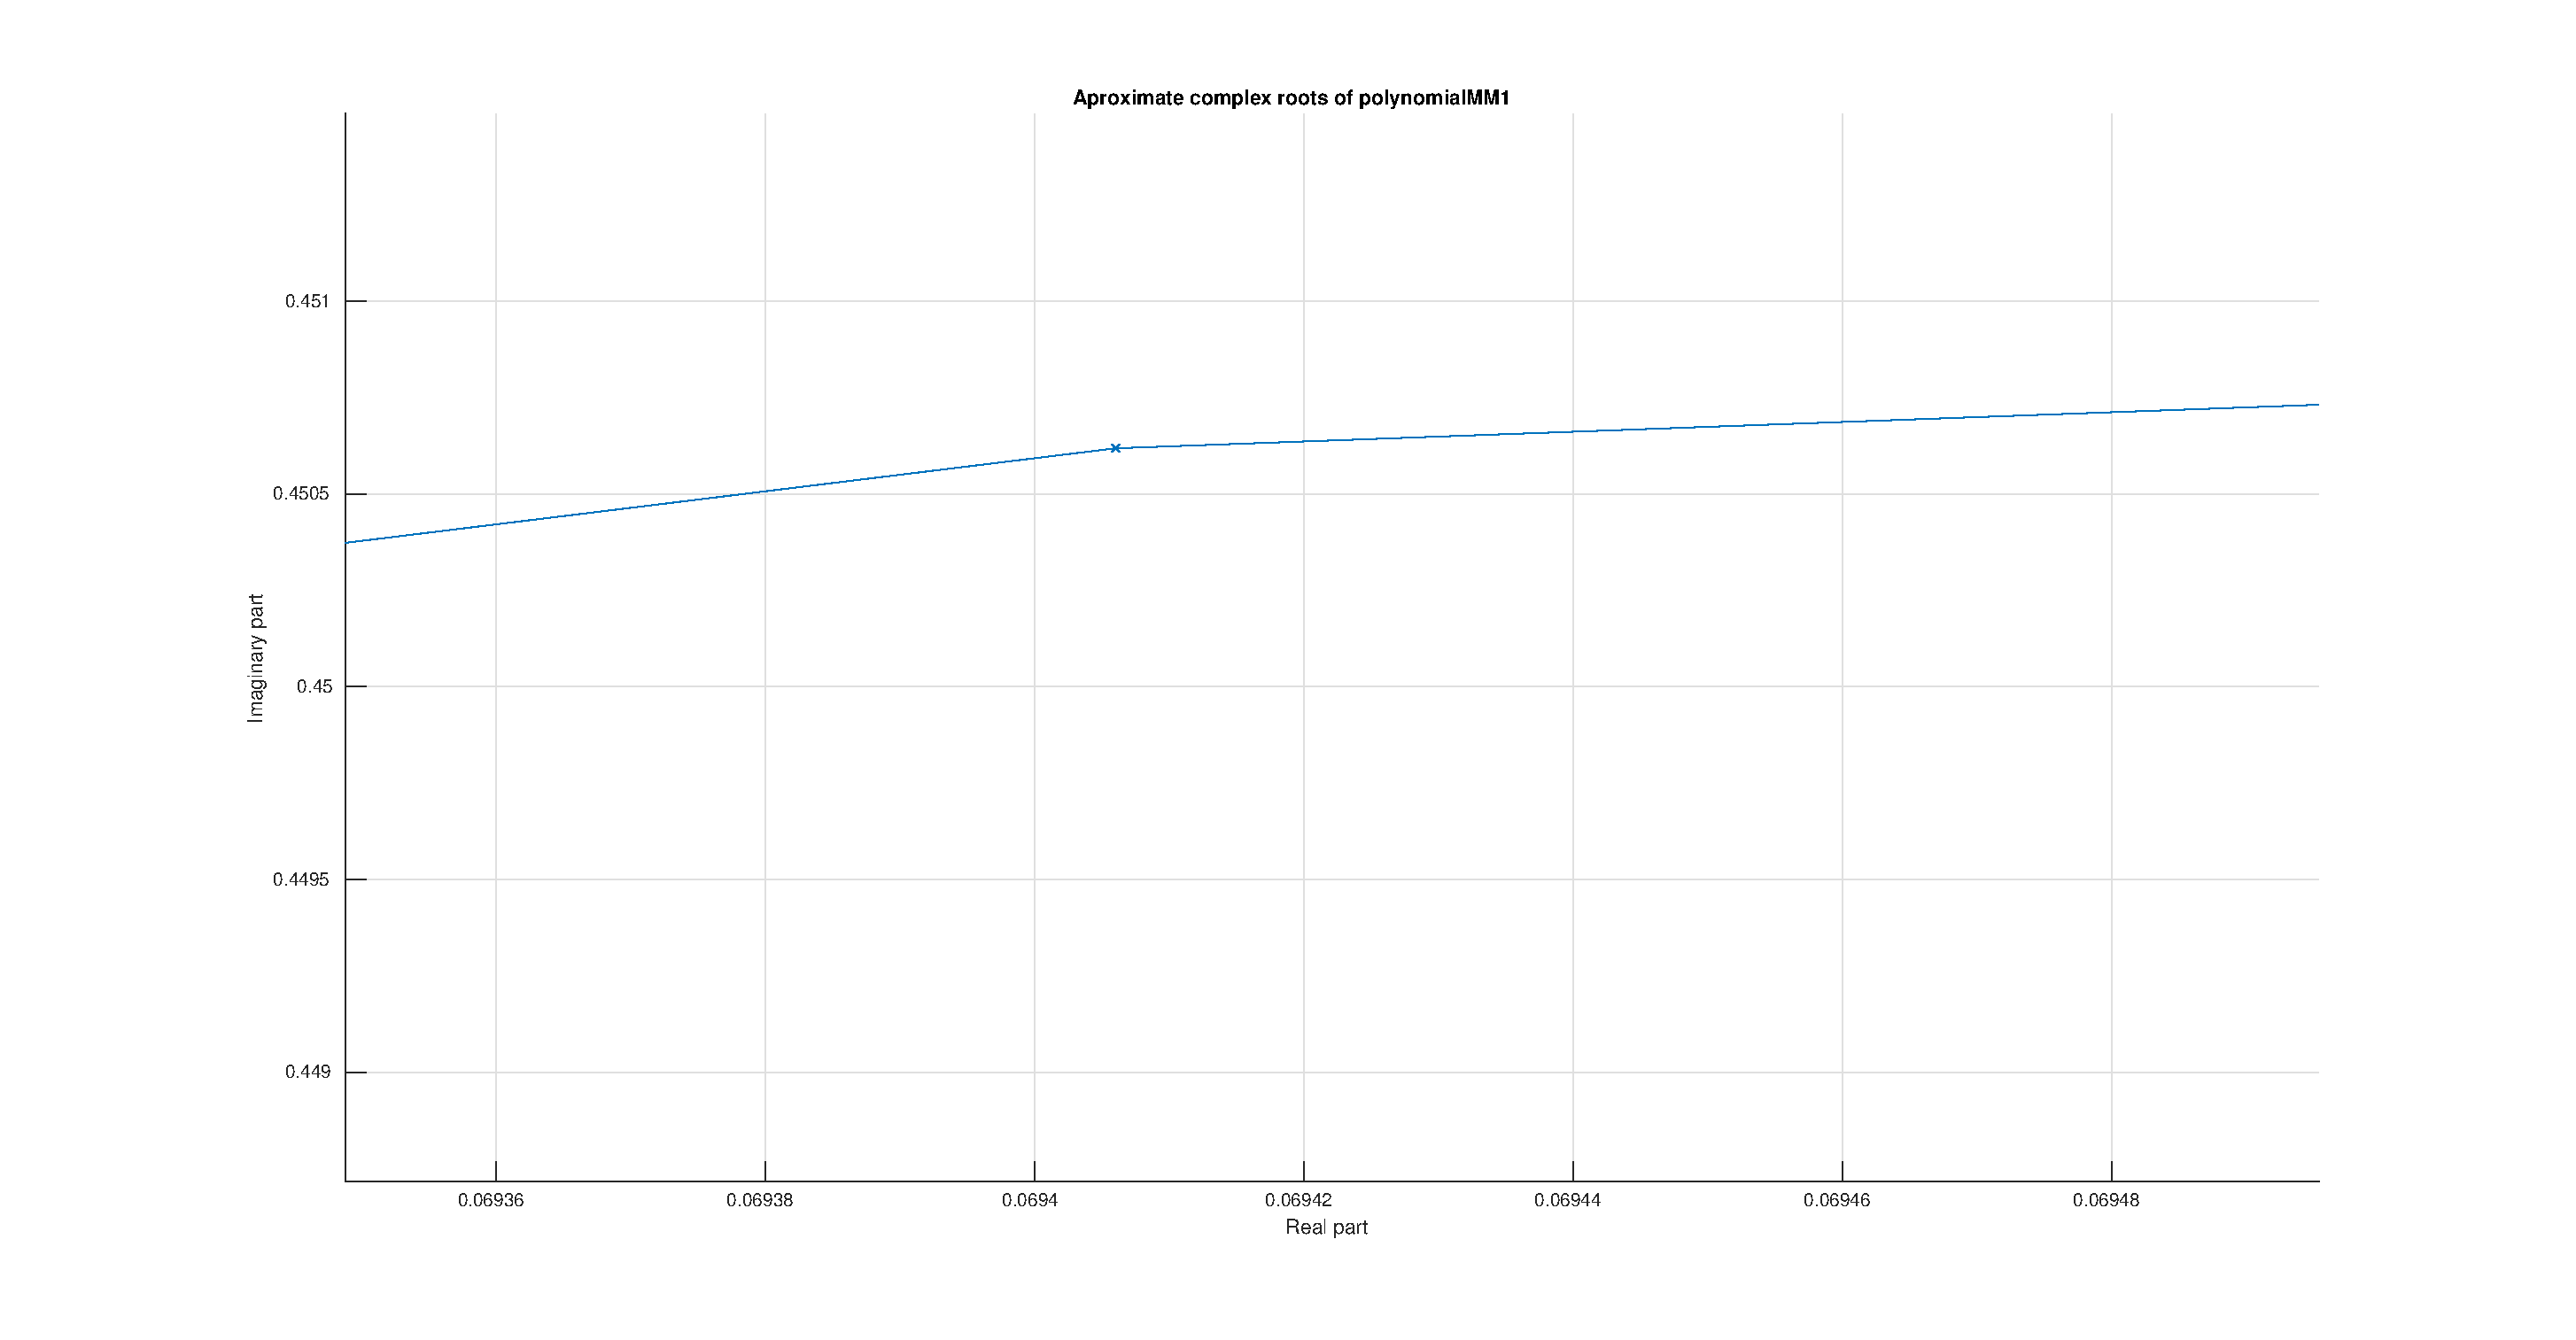
\includegraphics[scale=0.25]{task2mm1complexmiddle.eps}
\end{center}

\begin{center}
   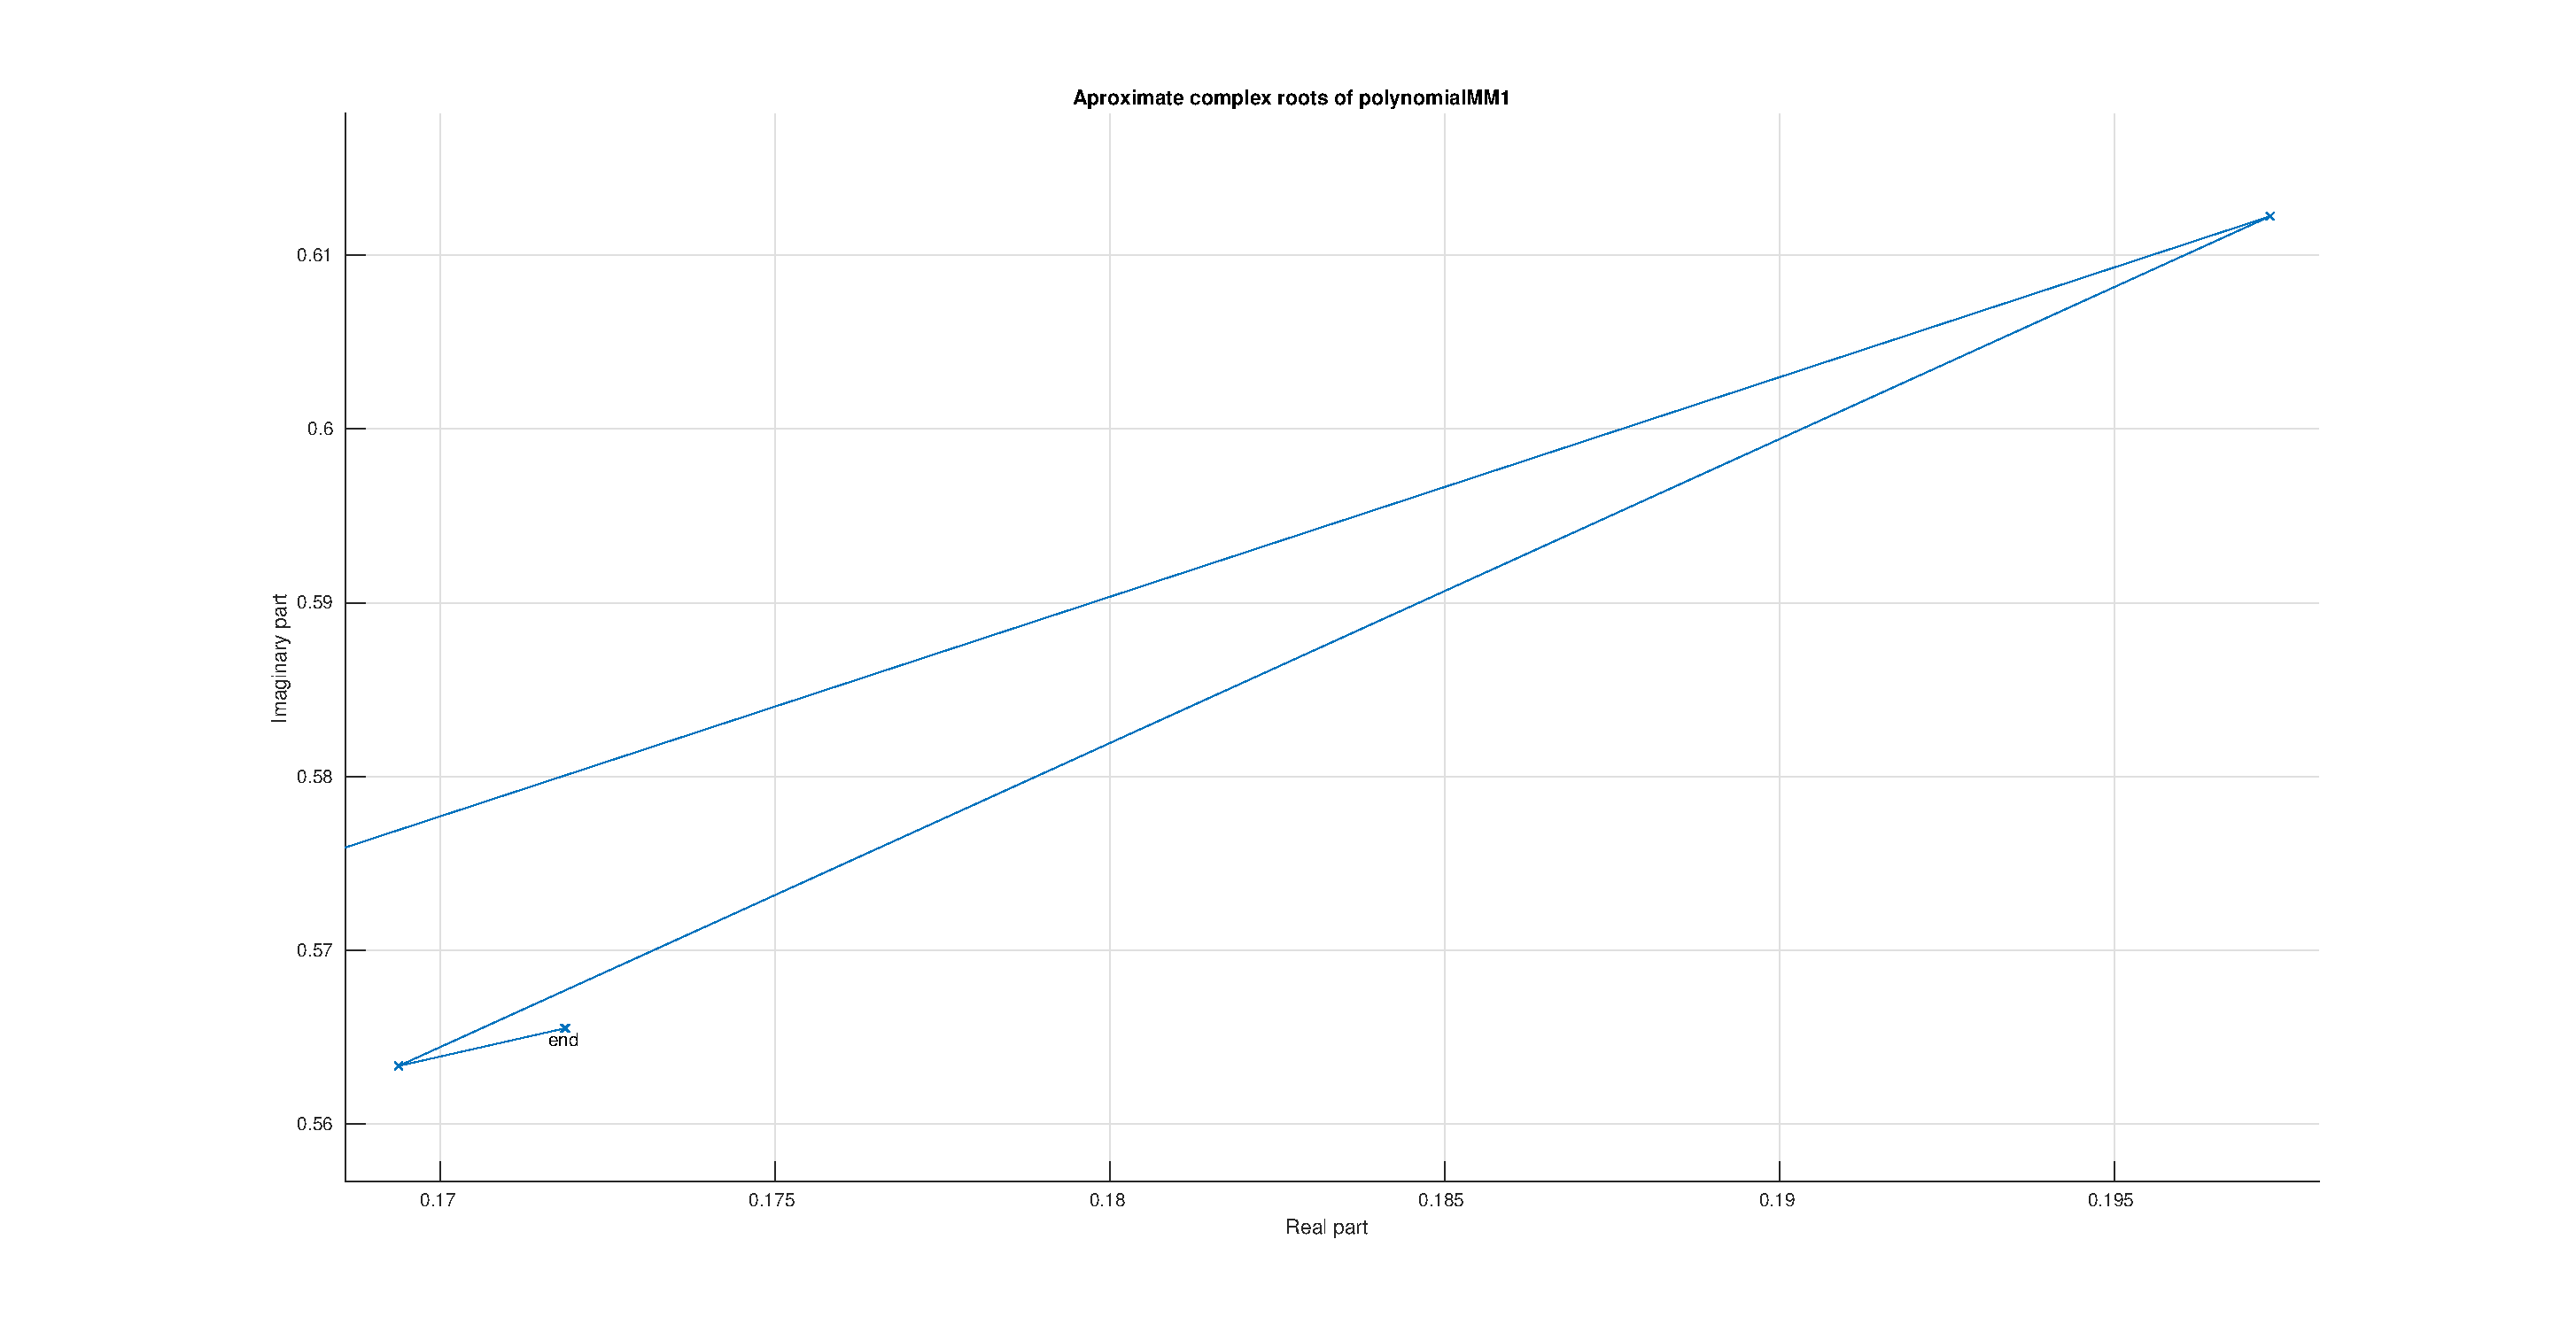
\includegraphics[scale=0.25]{task2mm1complexup.eps}
\end{center}

\subsection{Graphs for MM2}
\begin{center}
   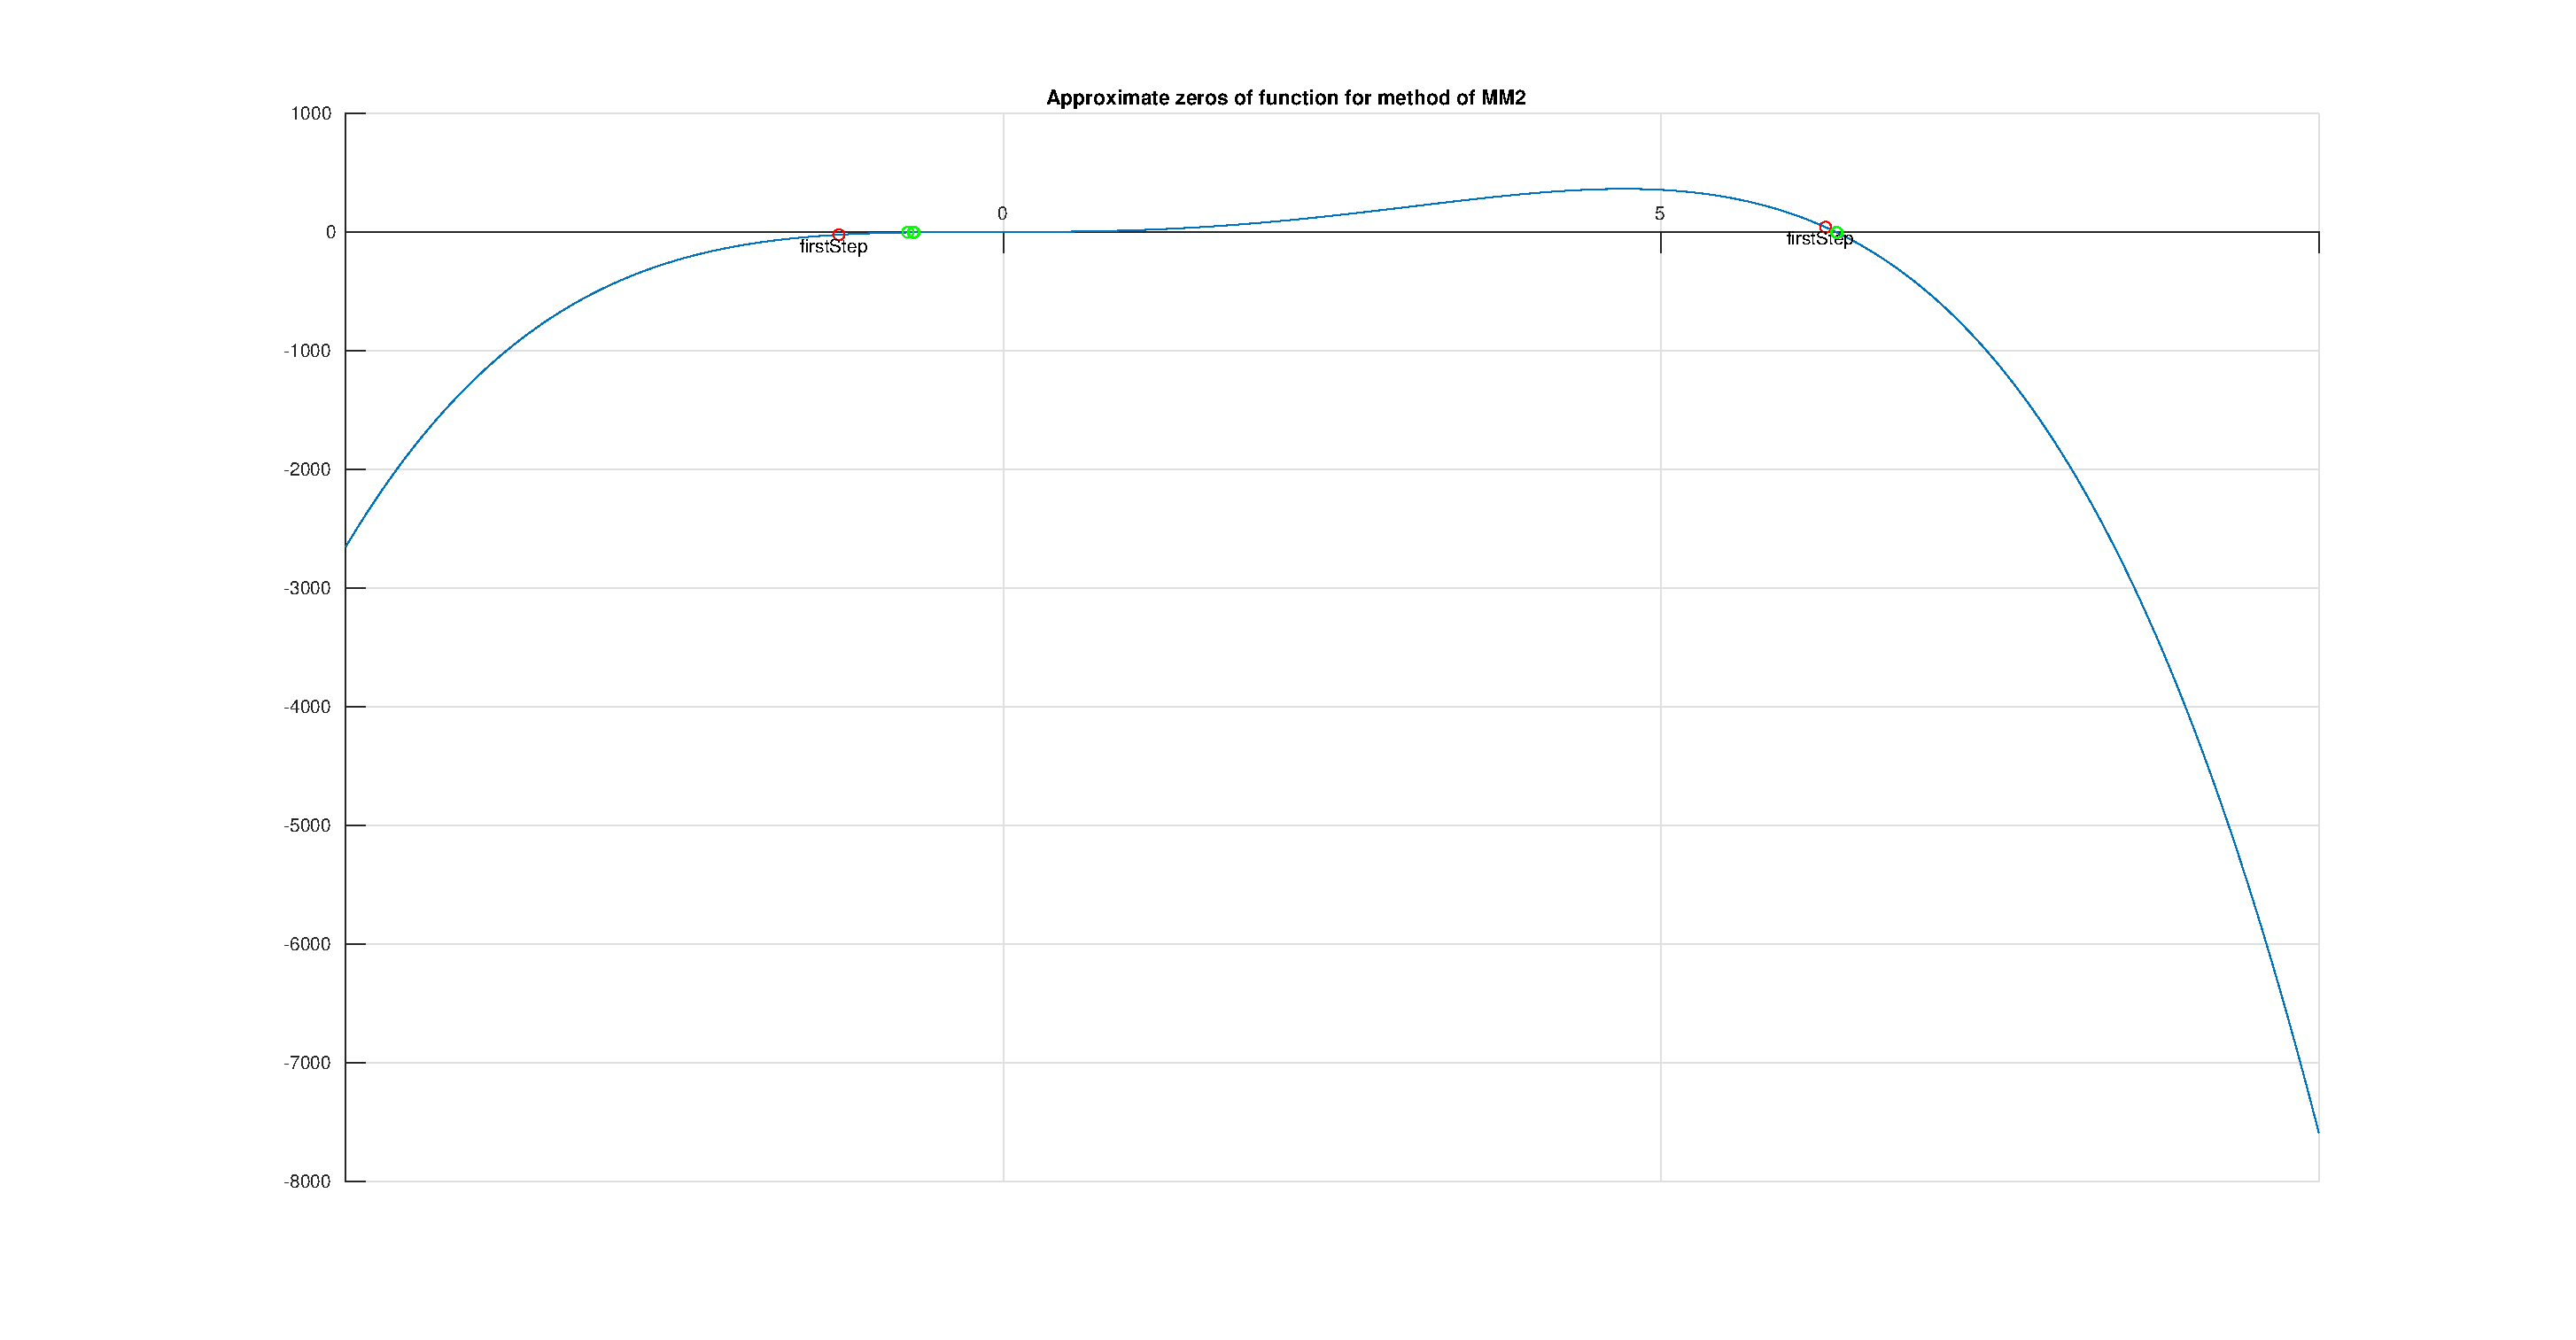
\includegraphics[scale=0.25]{task2mm2realoverall.eps}
\end{center}

\begin{center}
   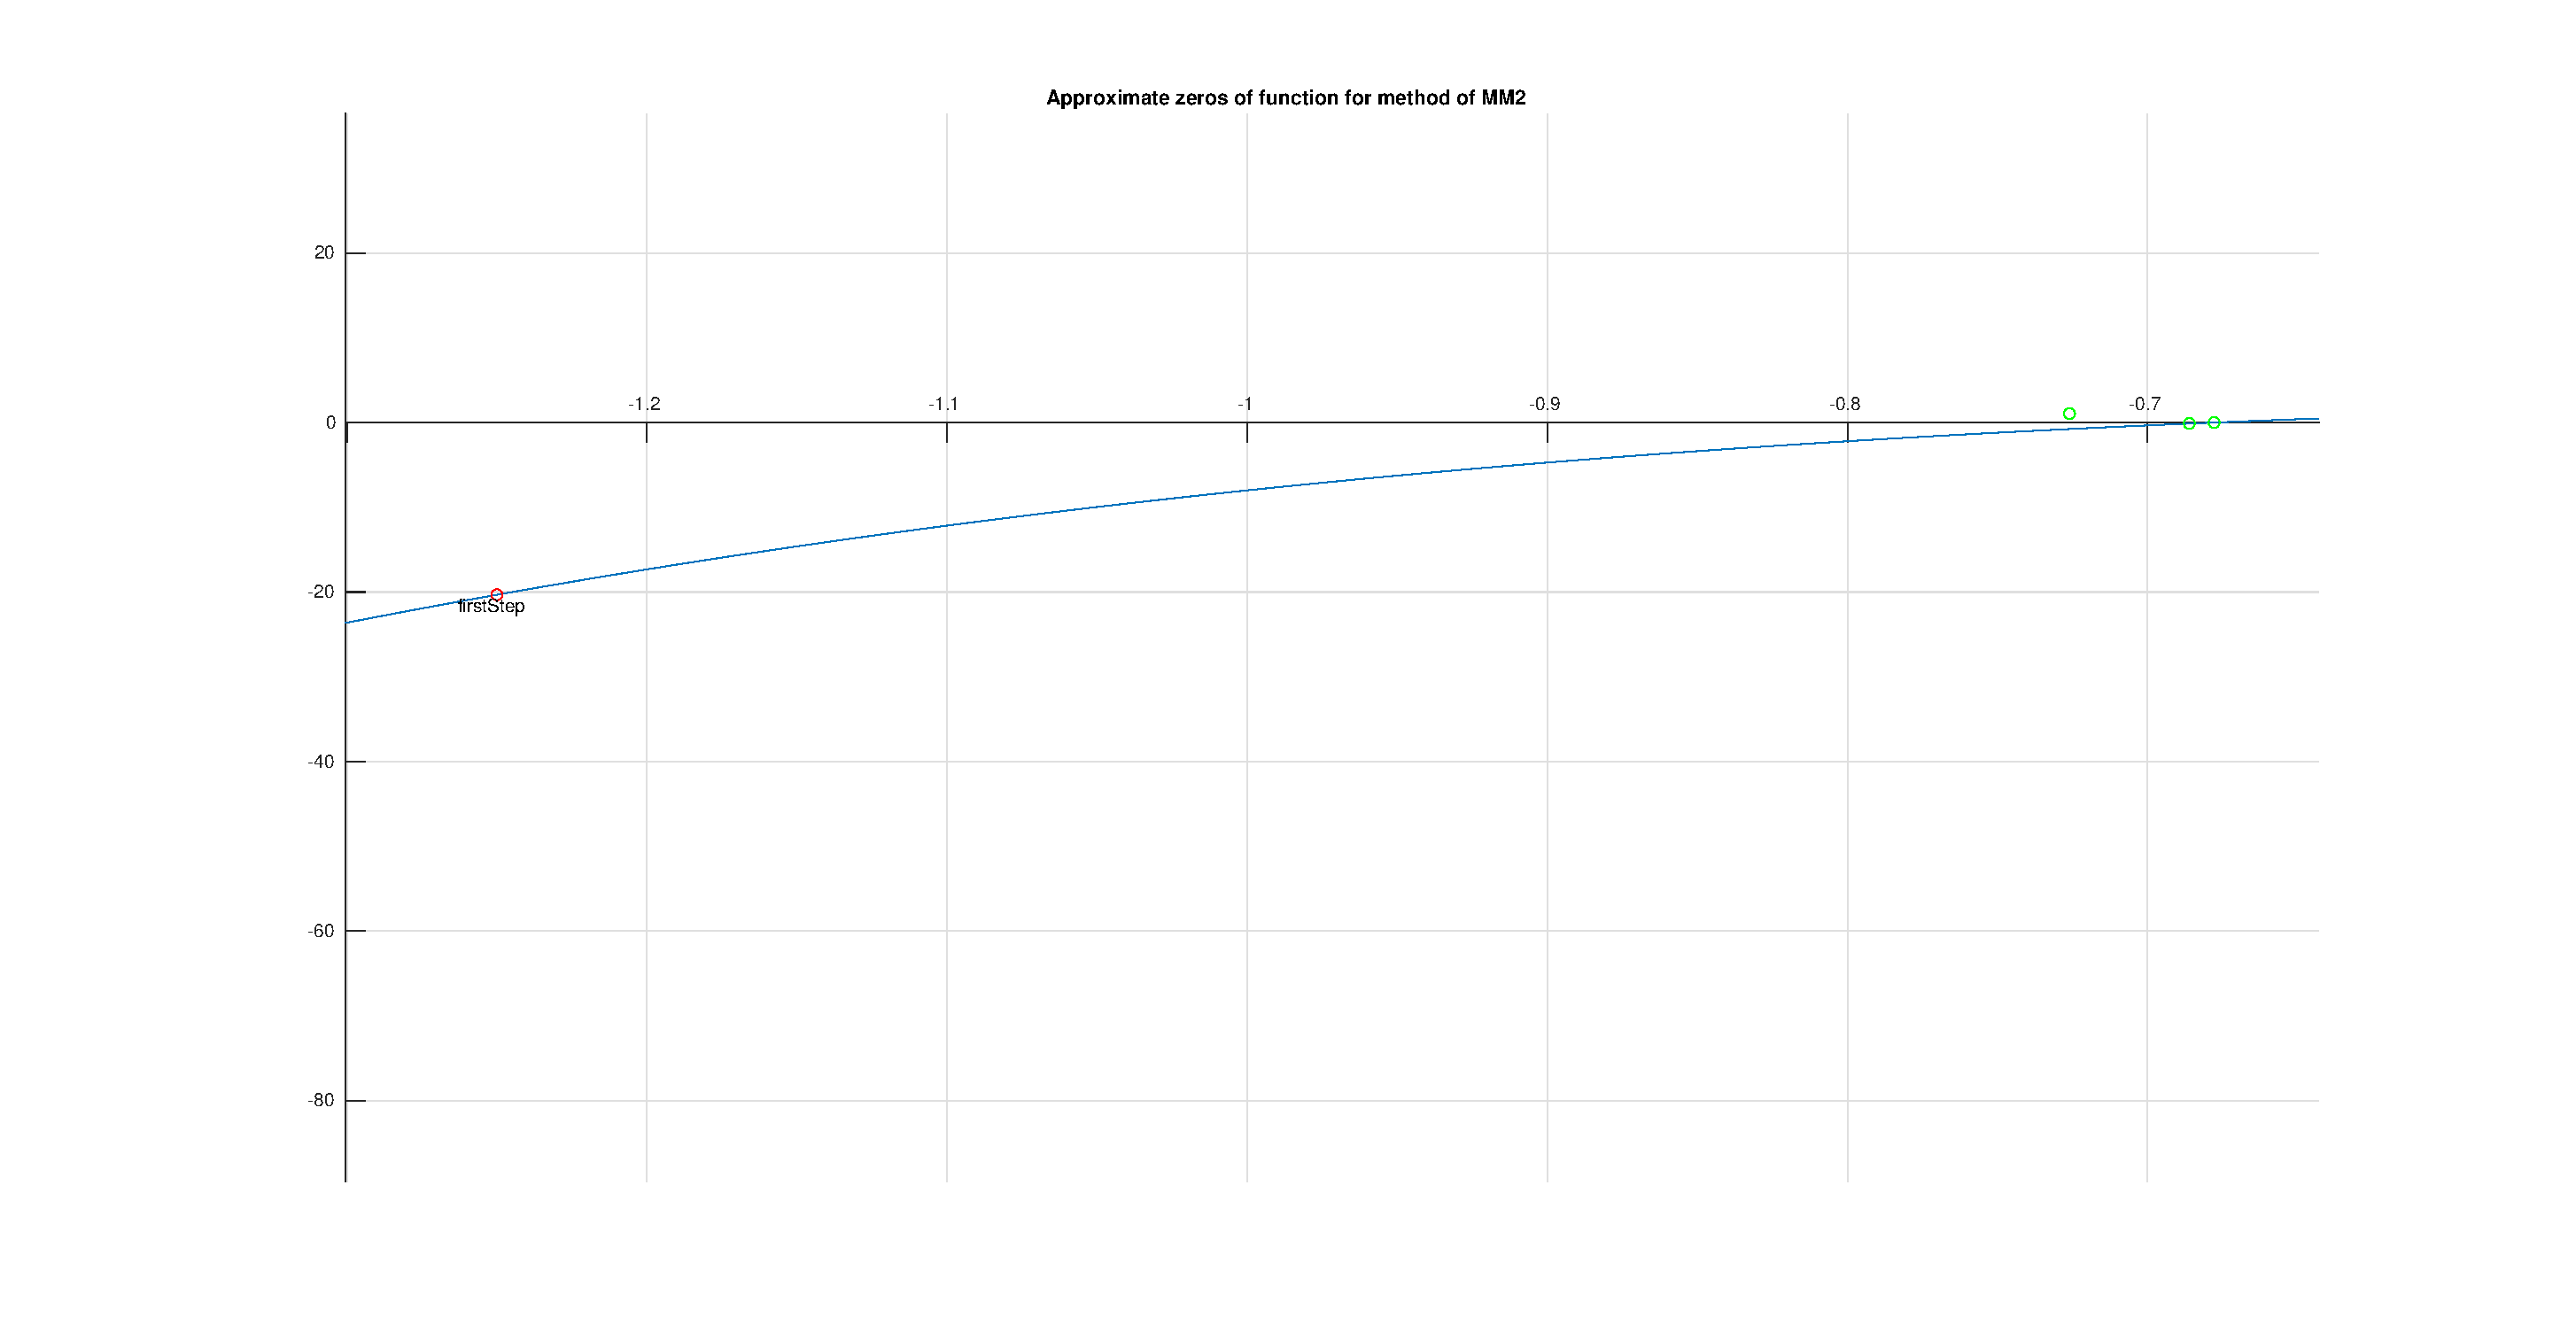
\includegraphics[scale=0.25]{task2mm2realleft.eps}
\end{center}

\begin{center}
   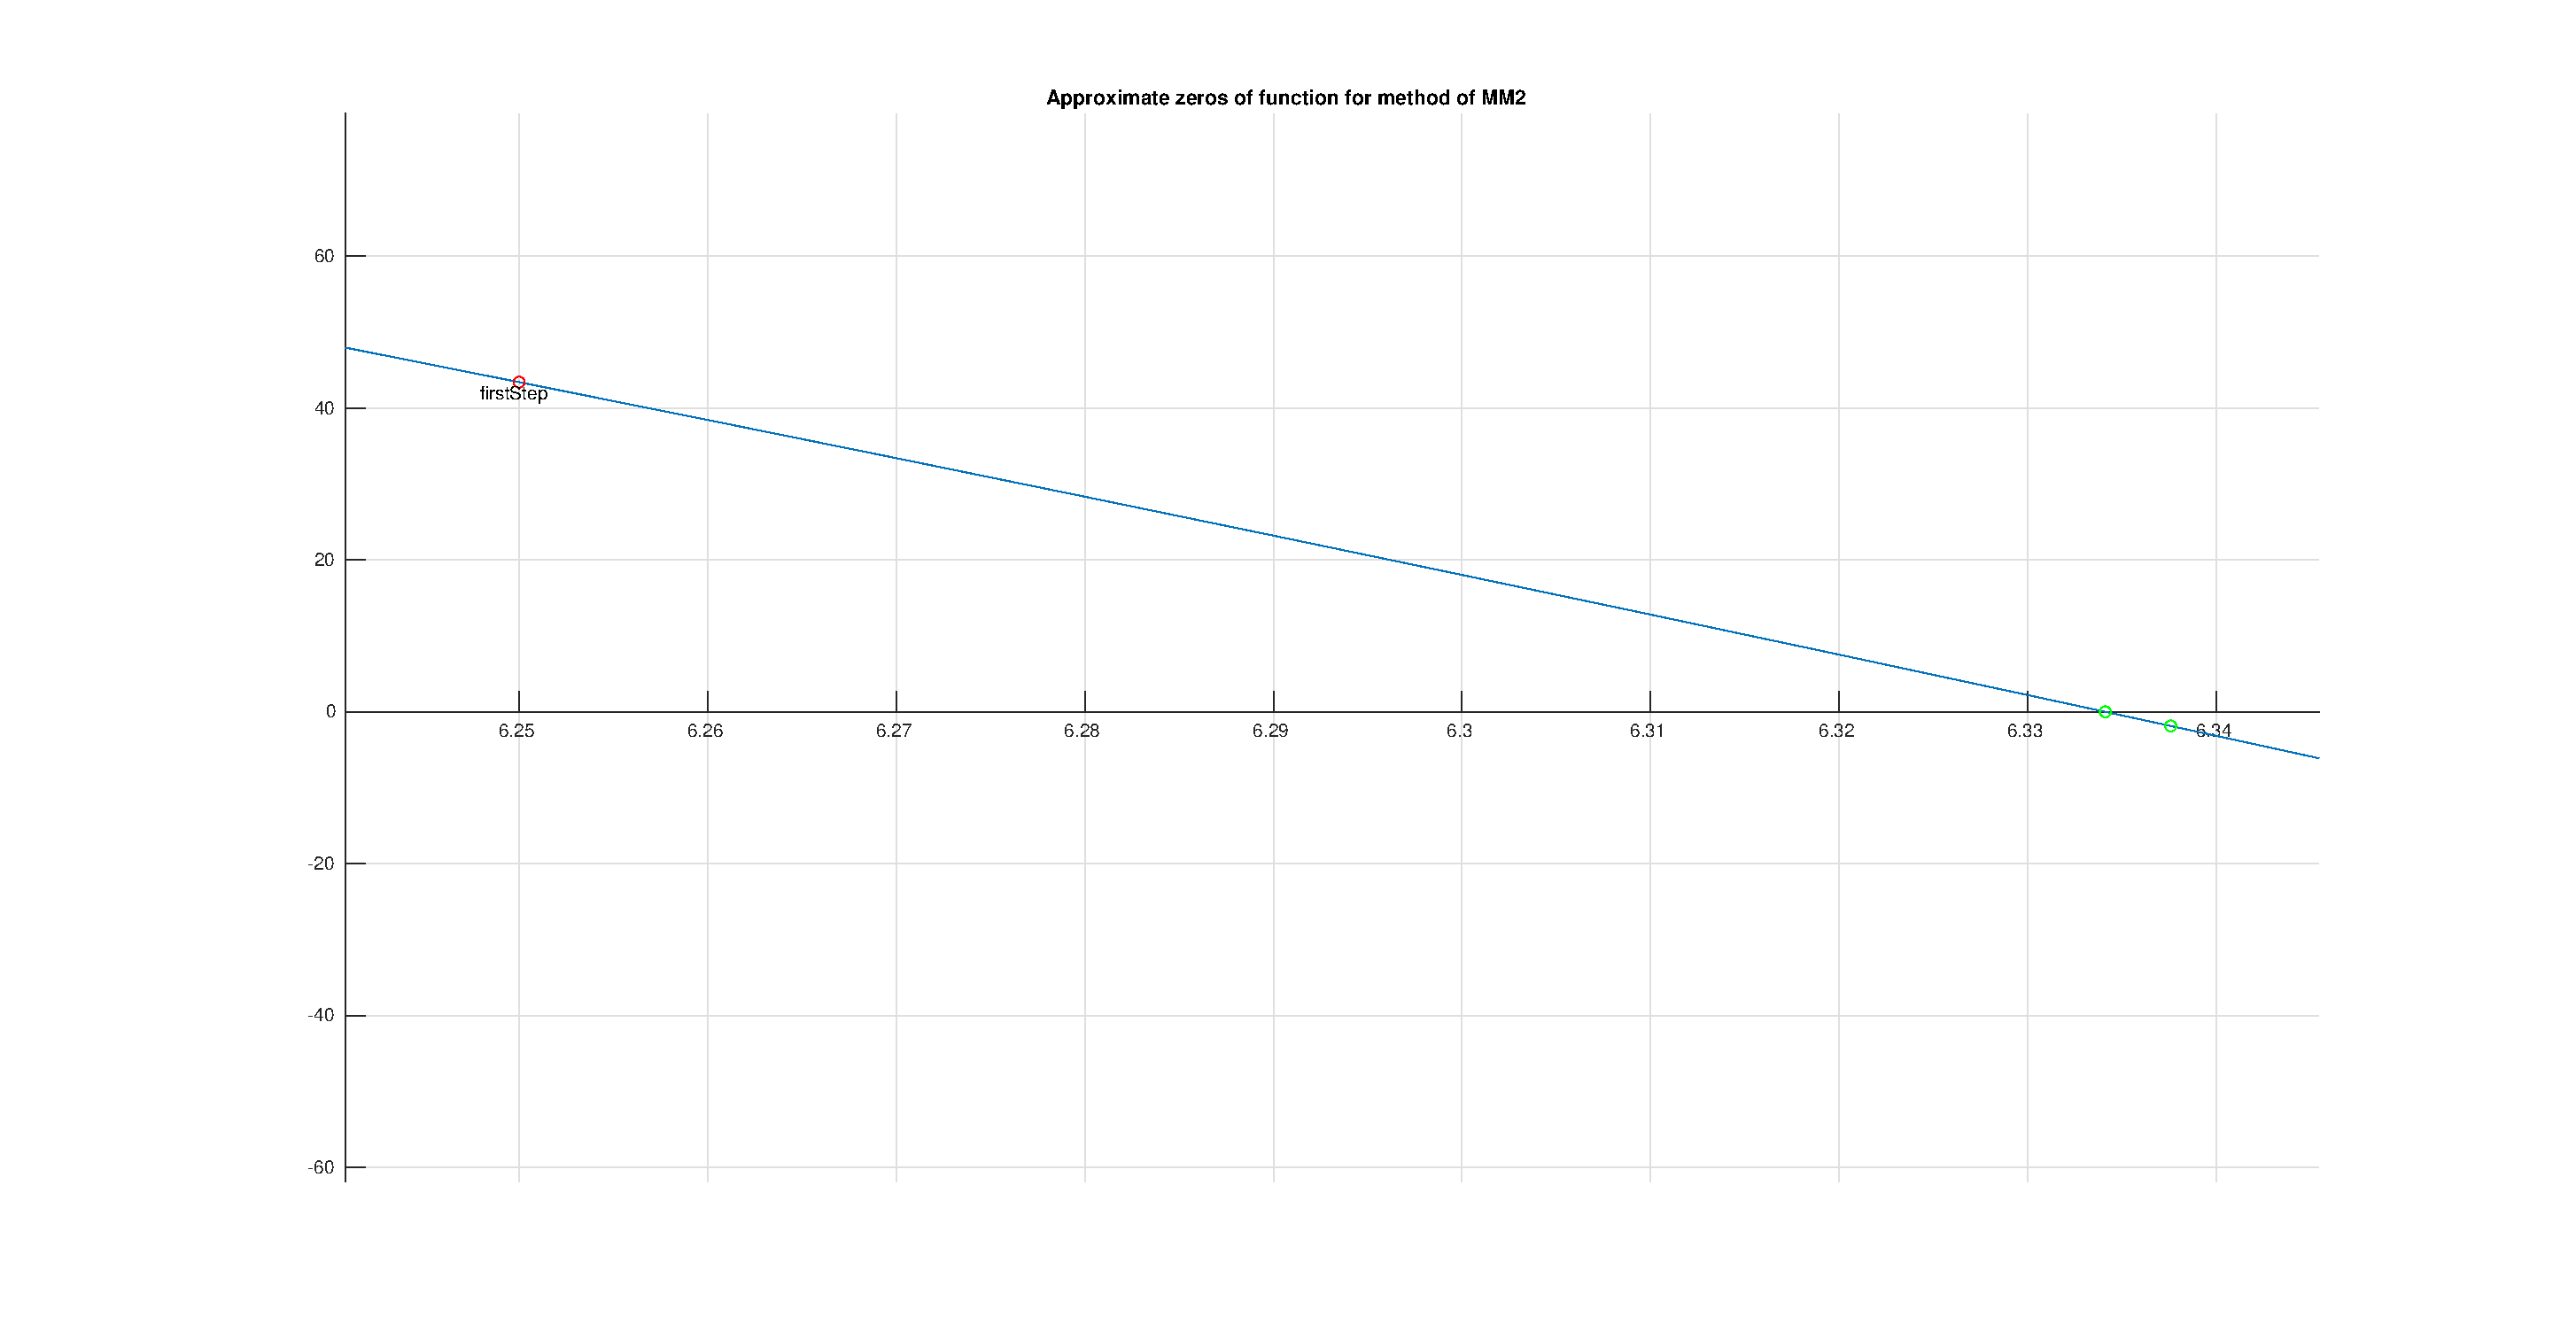
\includegraphics[scale=0.25]{task2mm2realright.eps}
\end{center}

\begin{center}
   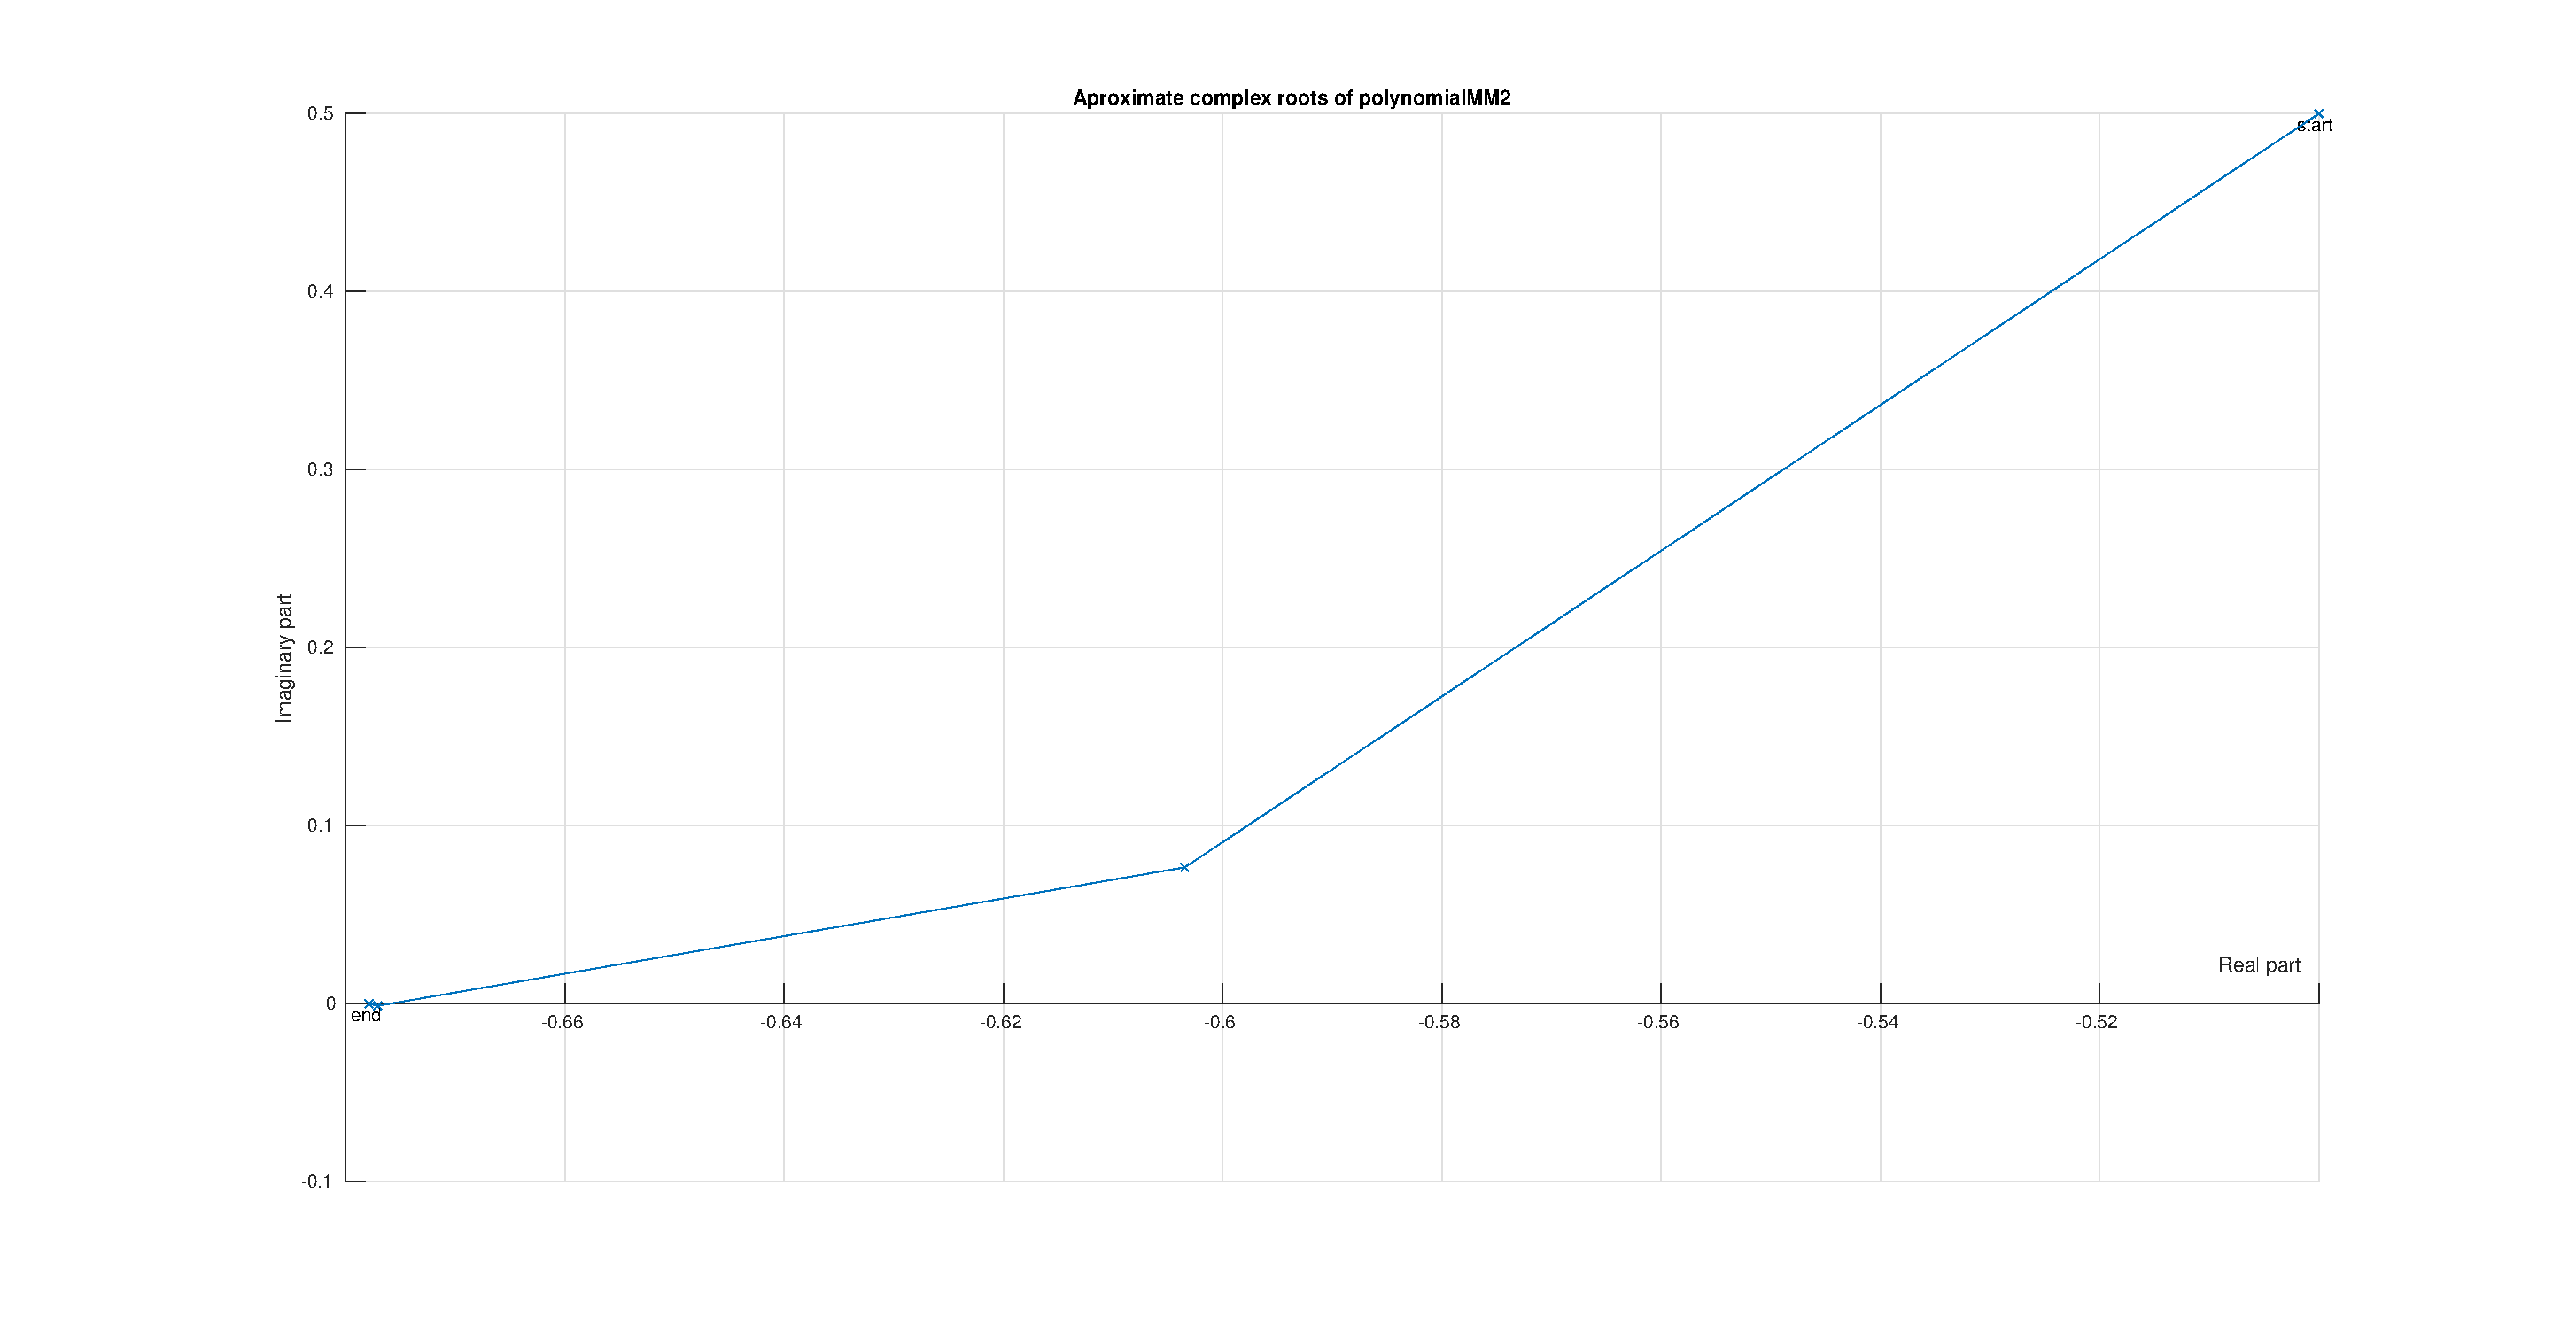
\includegraphics[scale=0.25]{task2mm2complexoverall.eps}
\end{center}

\begin{center}
   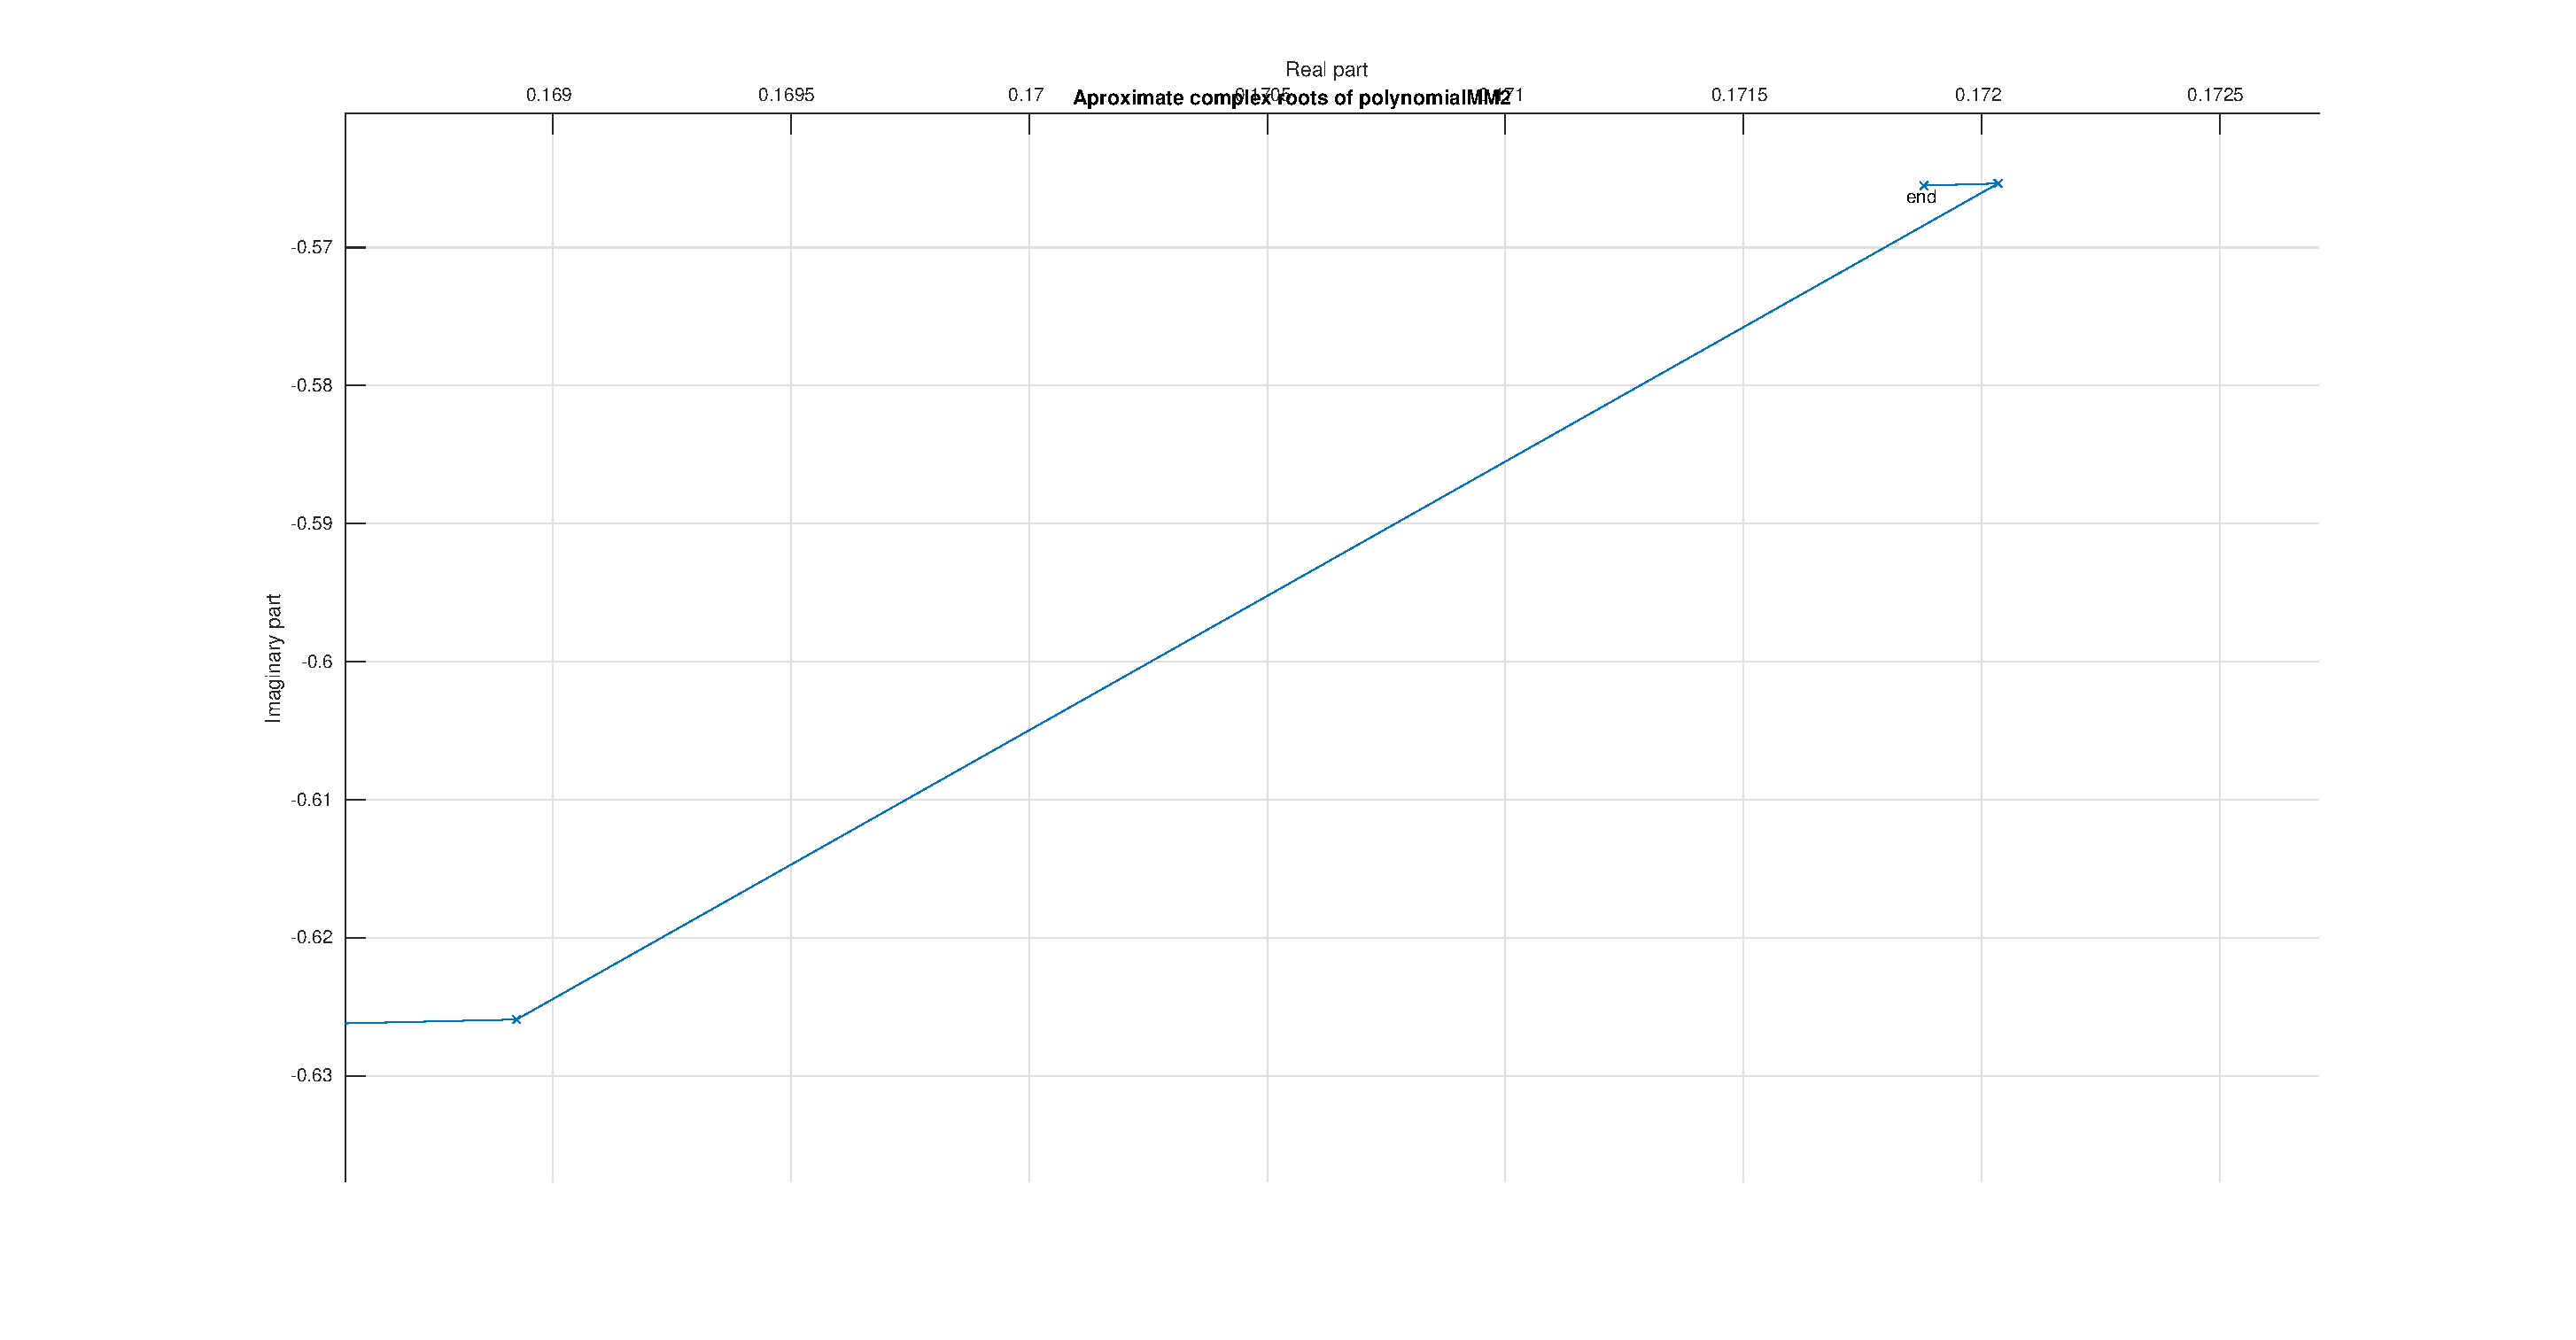
\includegraphics[scale=0.25]{task2mm2complexright.eps}
\end{center}

\begin{center}
   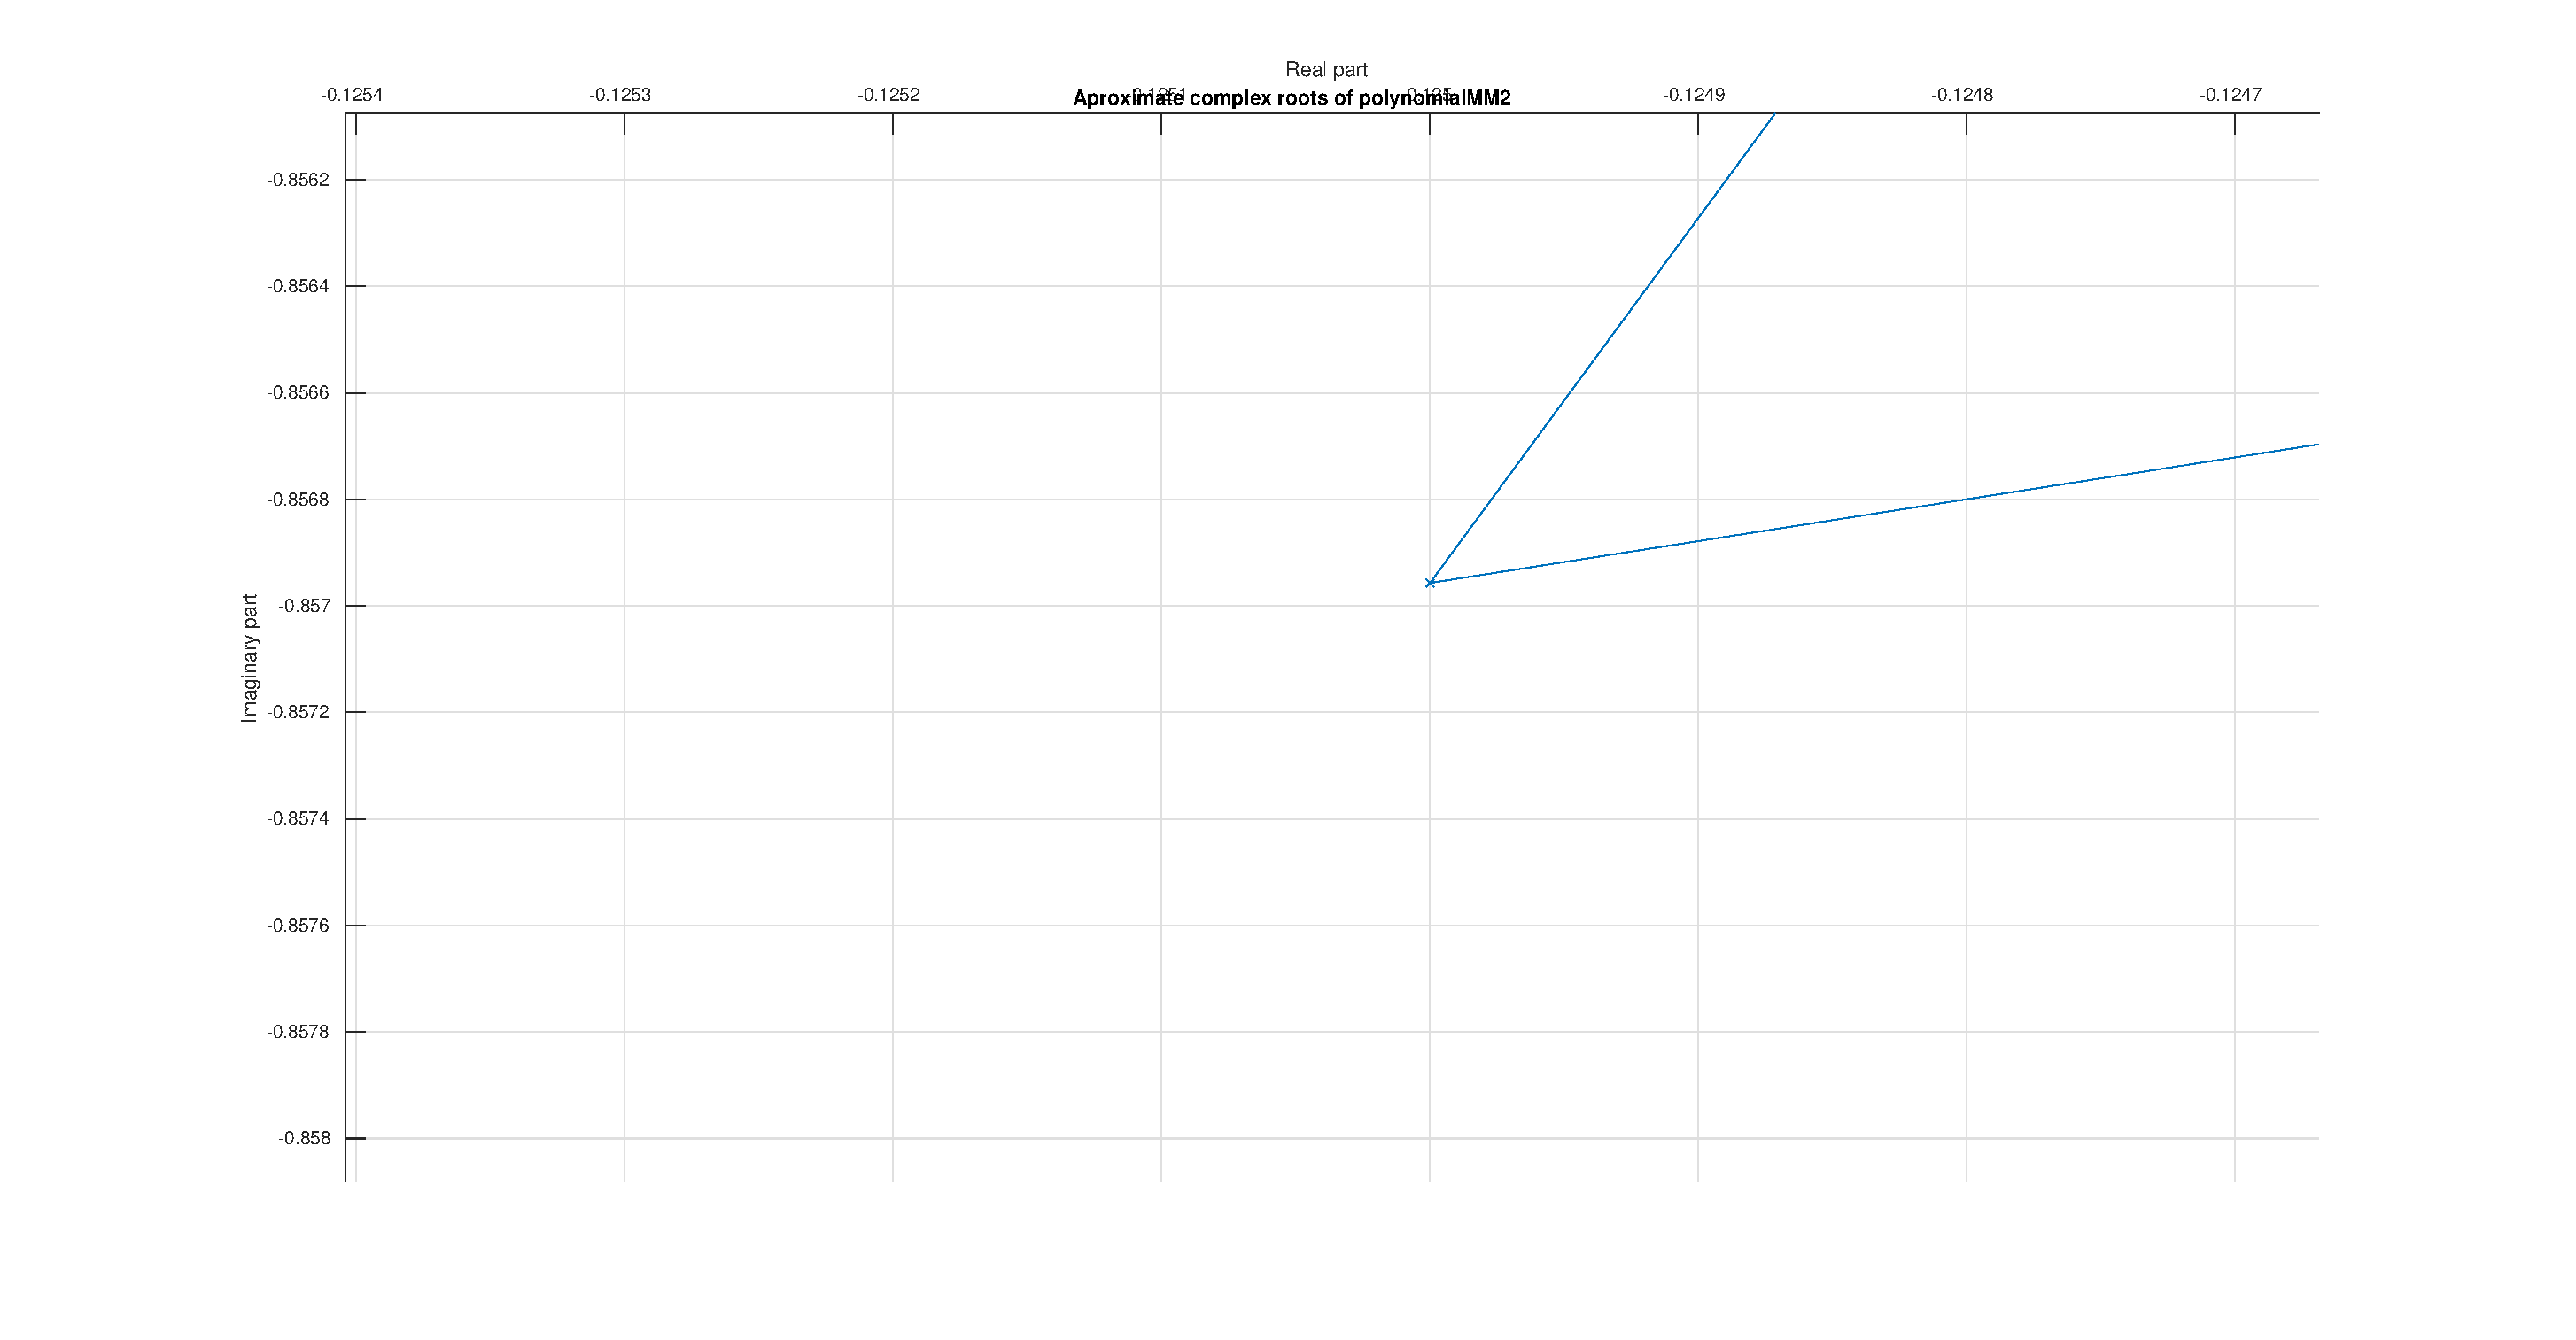
\includegraphics[scale=0.25]{task2mm2complexleft.eps}
\end{center}

\begin{center}
   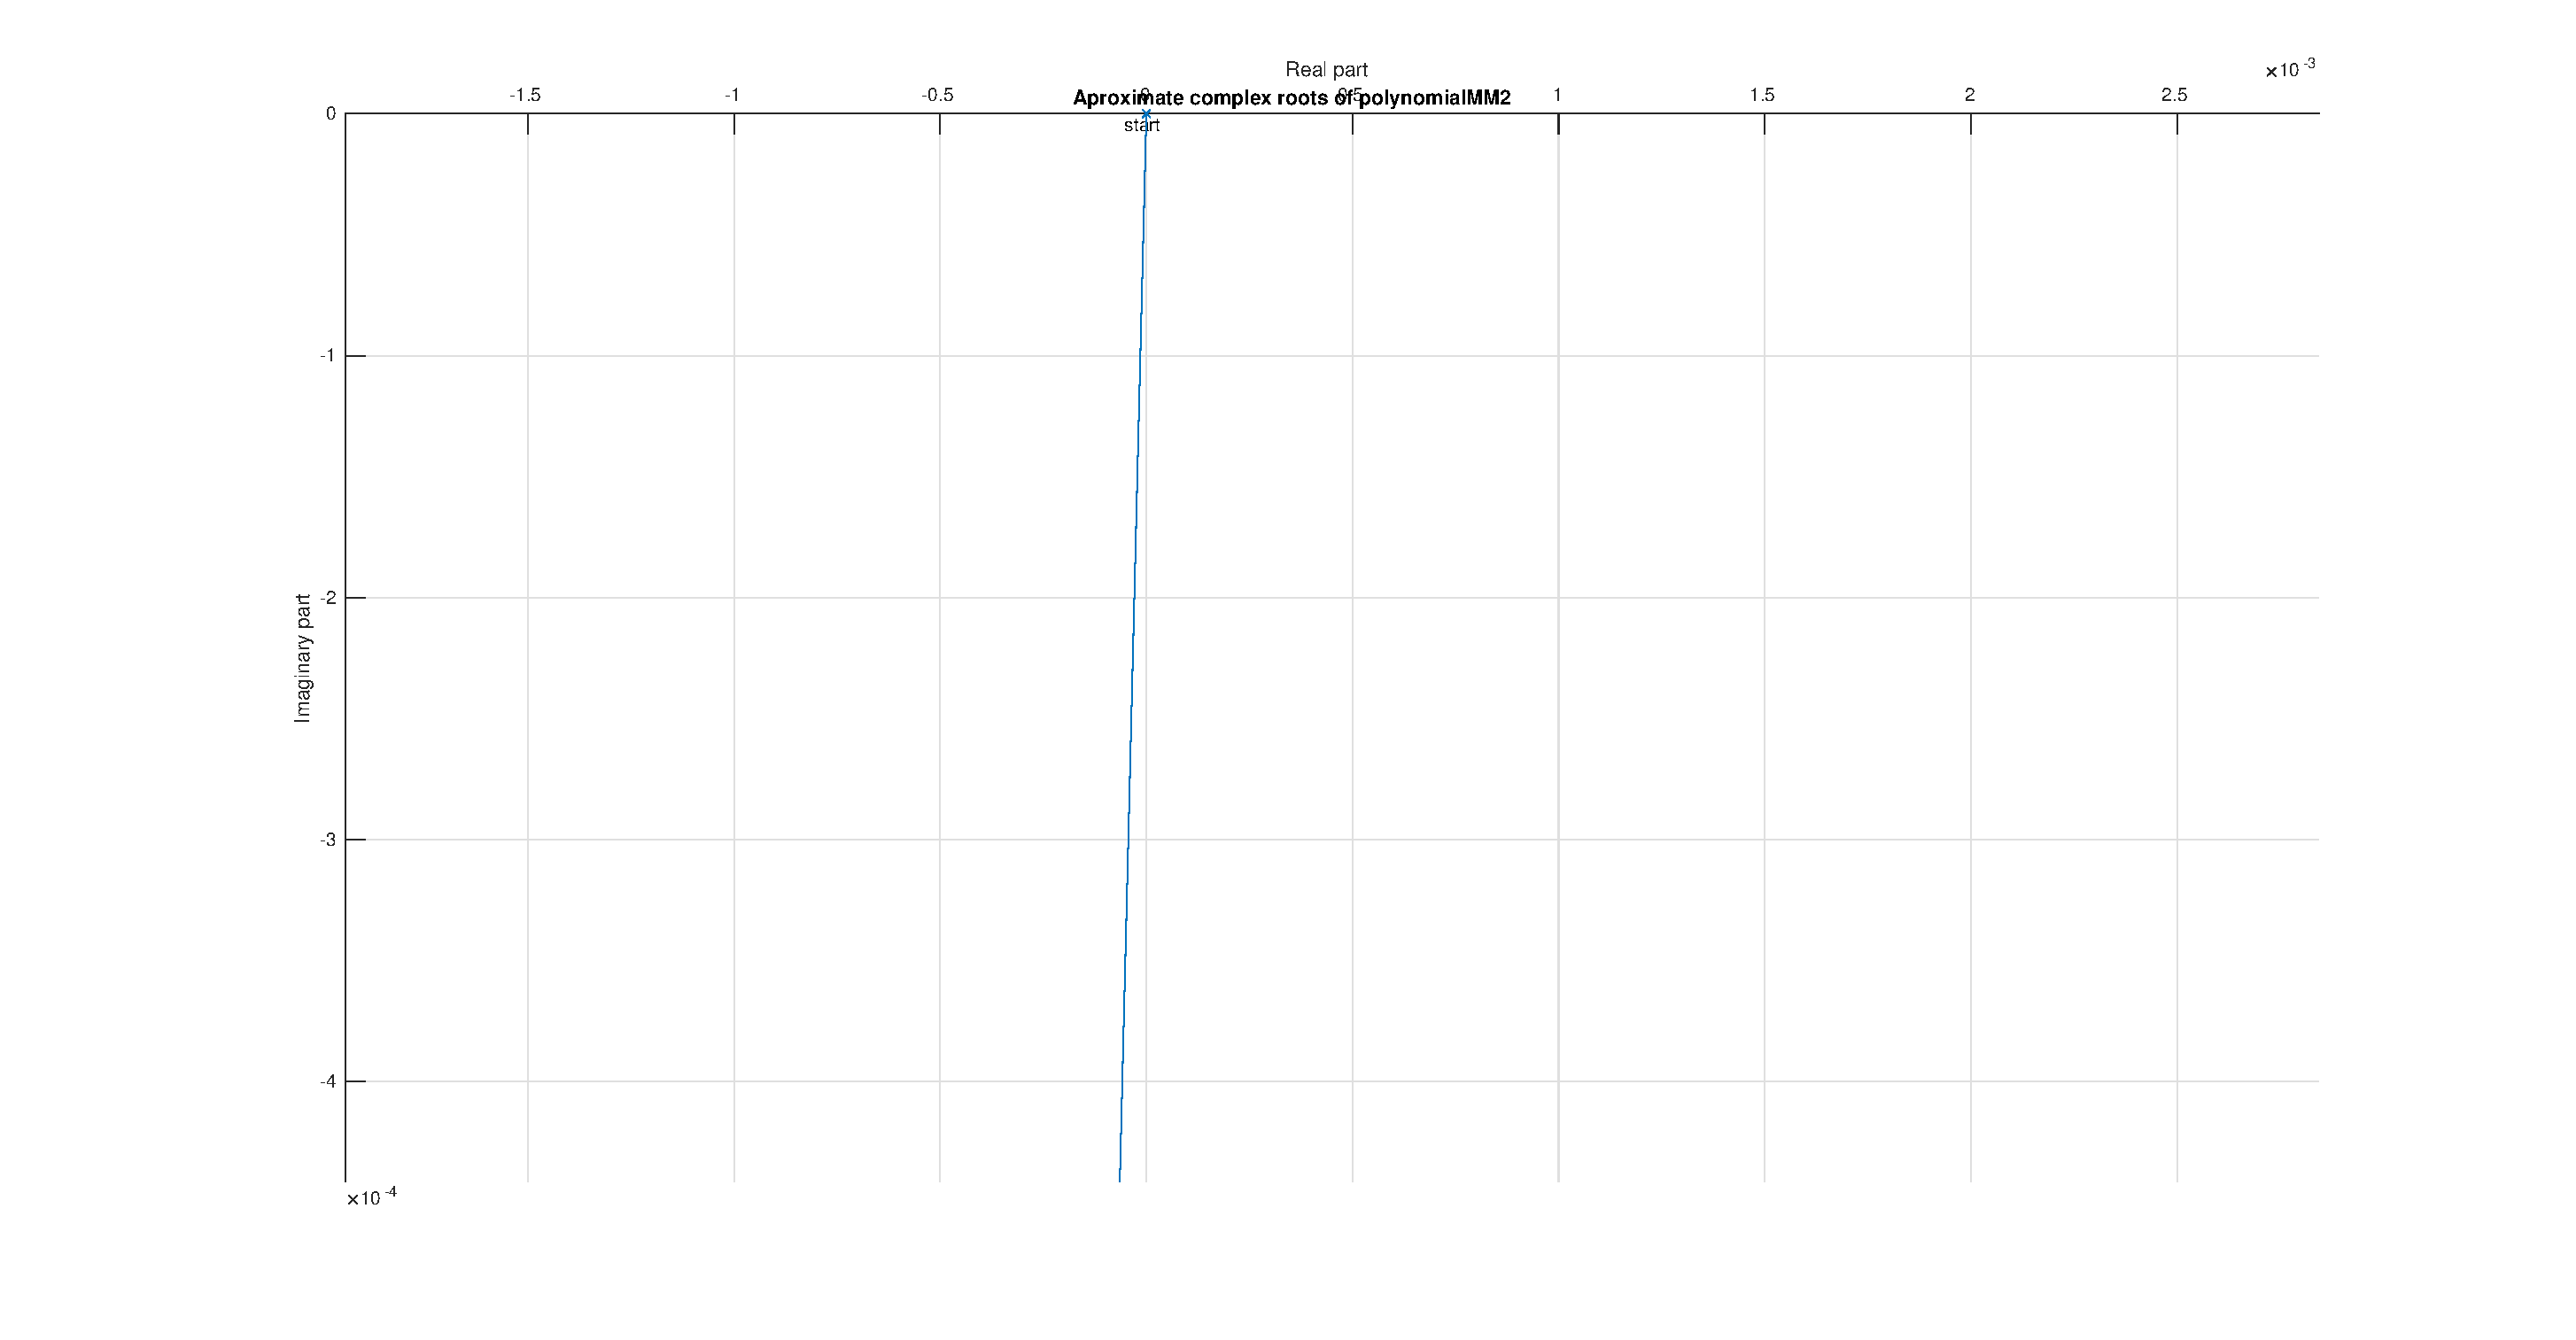
\includegraphics[scale=0.25]{task2mm2complexup.eps}
\end{center}

\subsection{Tables for MM1}
\begin{center}
  \begin{tabular}{| c  c c |}
\hline
Iteration & root         & f(root) \\
\hline
1    &     -1.25  &        -20.32 \\
\hline
2    &   -1.0009  &       -8.0351 \\
\hline
3    &  -0.76855  &       -1.5512 \\
\hline
4    &  -0.63496  &       0.58064 \\
\hline
5    &  -0.67945  &     -0.023155 \\
\hline
6    & -0.67788   &  -0.00010725 \\
\hline
7    & -0.67787   &  -8.6306e-09 \\
\hline
8    &  -0.67787  &             0 \\
\hline
\hline

\end{tabular}
\end{center}

\begin{center}
  \begin{tabular}{| c  c c |}
\hline
Iteration & root         & f(root) \\
\hline
1   &     6.25   &        43.43 \\
\hline
2   &   6.3257   &       4.4966 \\
\hline
3   &  6.3341    &   0.033379 \\
\hline
4   &   6.3341   &  -1.6916e-06 \\
\hline
5   &   6.3341   &  -7.1942e-14 \\
\hline

\hline

\end{tabular}
\end{center}

\begin{center}
  \begin{tabular}{| c  c c |}
\hline
Iteration & root         & f(root) \\
\hline
1   &            0+0i         &             3   \\
\hline
2   &  -0.0072549-0.12193i    &       2.9384   \\
\hline
3   &     0.069406-0.45062i   &       1.7235  \\
\hline
4   &      0.19733-0.61224i   &      0.82578   \\
\hline
5   &     0.16937-0.56334i    &     0.047116   \\
\hline
6   &      0.17186-0.56551i   &     0.0003142   \\
\hline
7   &      0.17188-0.56551i   &    4.4741e-08  \\
\hline
8   &      0.17188-0.56551i   &    2.6645e-15    \\
\hline
9   &      0.17188-0.56551i   &             0   \\
\hline
\hline

\end{tabular}
\end{center}

\subsection{Tables for MM2}
\begin{center}
  \begin{tabular}{| c  c c |}
\hline
Iteration & root         & f(root) \\
\hline
1  &       -1.25+0i         &         -20.32+0i    \\
\hline
2  &    -0.72604-0.25326i   &         1.0515-4.0744i  \\
\hline
3  &   -0.68613-0.01483i    &      -0.11667-0.22303i   \\
\hline
4  &   -0.67788+2.5407e-06i &   -0.00010163+3.7123e-05i \\
\hline
5  &    -0.67787-8.0819e-13i &    1.4105e-11-1.1809e-11i \\
\hline
 \hline

\end{tabular}
\end{center}

\begin{center}
  \begin{tabular}{| c  c c |}
\hline
Iteration & root         & f(root) \\
\hline
1   &     6.25    &       43.43 \\
\hline
2   &   6.3376    &     -1.8647 \\
\hline
3   &  6.3341     &  0.0029695 \\
\hline
4   &   6.3341    &  1.6294e-08 \\
\hline
5   &   6.3341    & -4.6896e-13 \\
\hline
\hline

\end{tabular}
\end{center}

\begin{center}
  \begin{tabular}{| c  c c |}
\hline
Iteration & root         & f(root) \\
\hline
1   &         0+0i          &            3 \\
\hline
2   &    -0.125+0.85696i    &       8.0341 \\
\hline
3   &   0.16892+0.62593i    &      0.94053 \\
\hline
4   &   0.17203+0.56536i    &    0.0031354  \\
\hline
5   &   0.17188+0.56551i    &   3.8615e-09  \\
\hline
6   &   0.17188+0.56551i    &            0  \\
\hline
\hline

\end{tabular}
\end{center}

\subsection{Comparison of results between MM1 and MM2}
As we can see MM2 method is much better, it took on average around 5 iterations for it to find a root with sufficient accuracy compared to around 7 iterations that MM1 needed to find roots.  MM1 is slightly more accurate with at least 10 times better accuary than MM2, there is also a big error in MM2 result which incorrectly denotes a number that should only have real part as an imaginary number. MM1 does not have this problem and shows root -0.67787 correctly. We can also observe that MM1 calculated complex root with a '-' between real and imaginary part and MM2 calculated complex root with a '+' between real and imaginary part. We can assume that in order to get all the complex roots we should use both of the methods.

We can also observe that on graphs with MM2 approaching the root faster than MM1 and MM1 being slightly more accurate.
\subsection{Comparison of results between Newton's method and MM2}

\begin{center}
   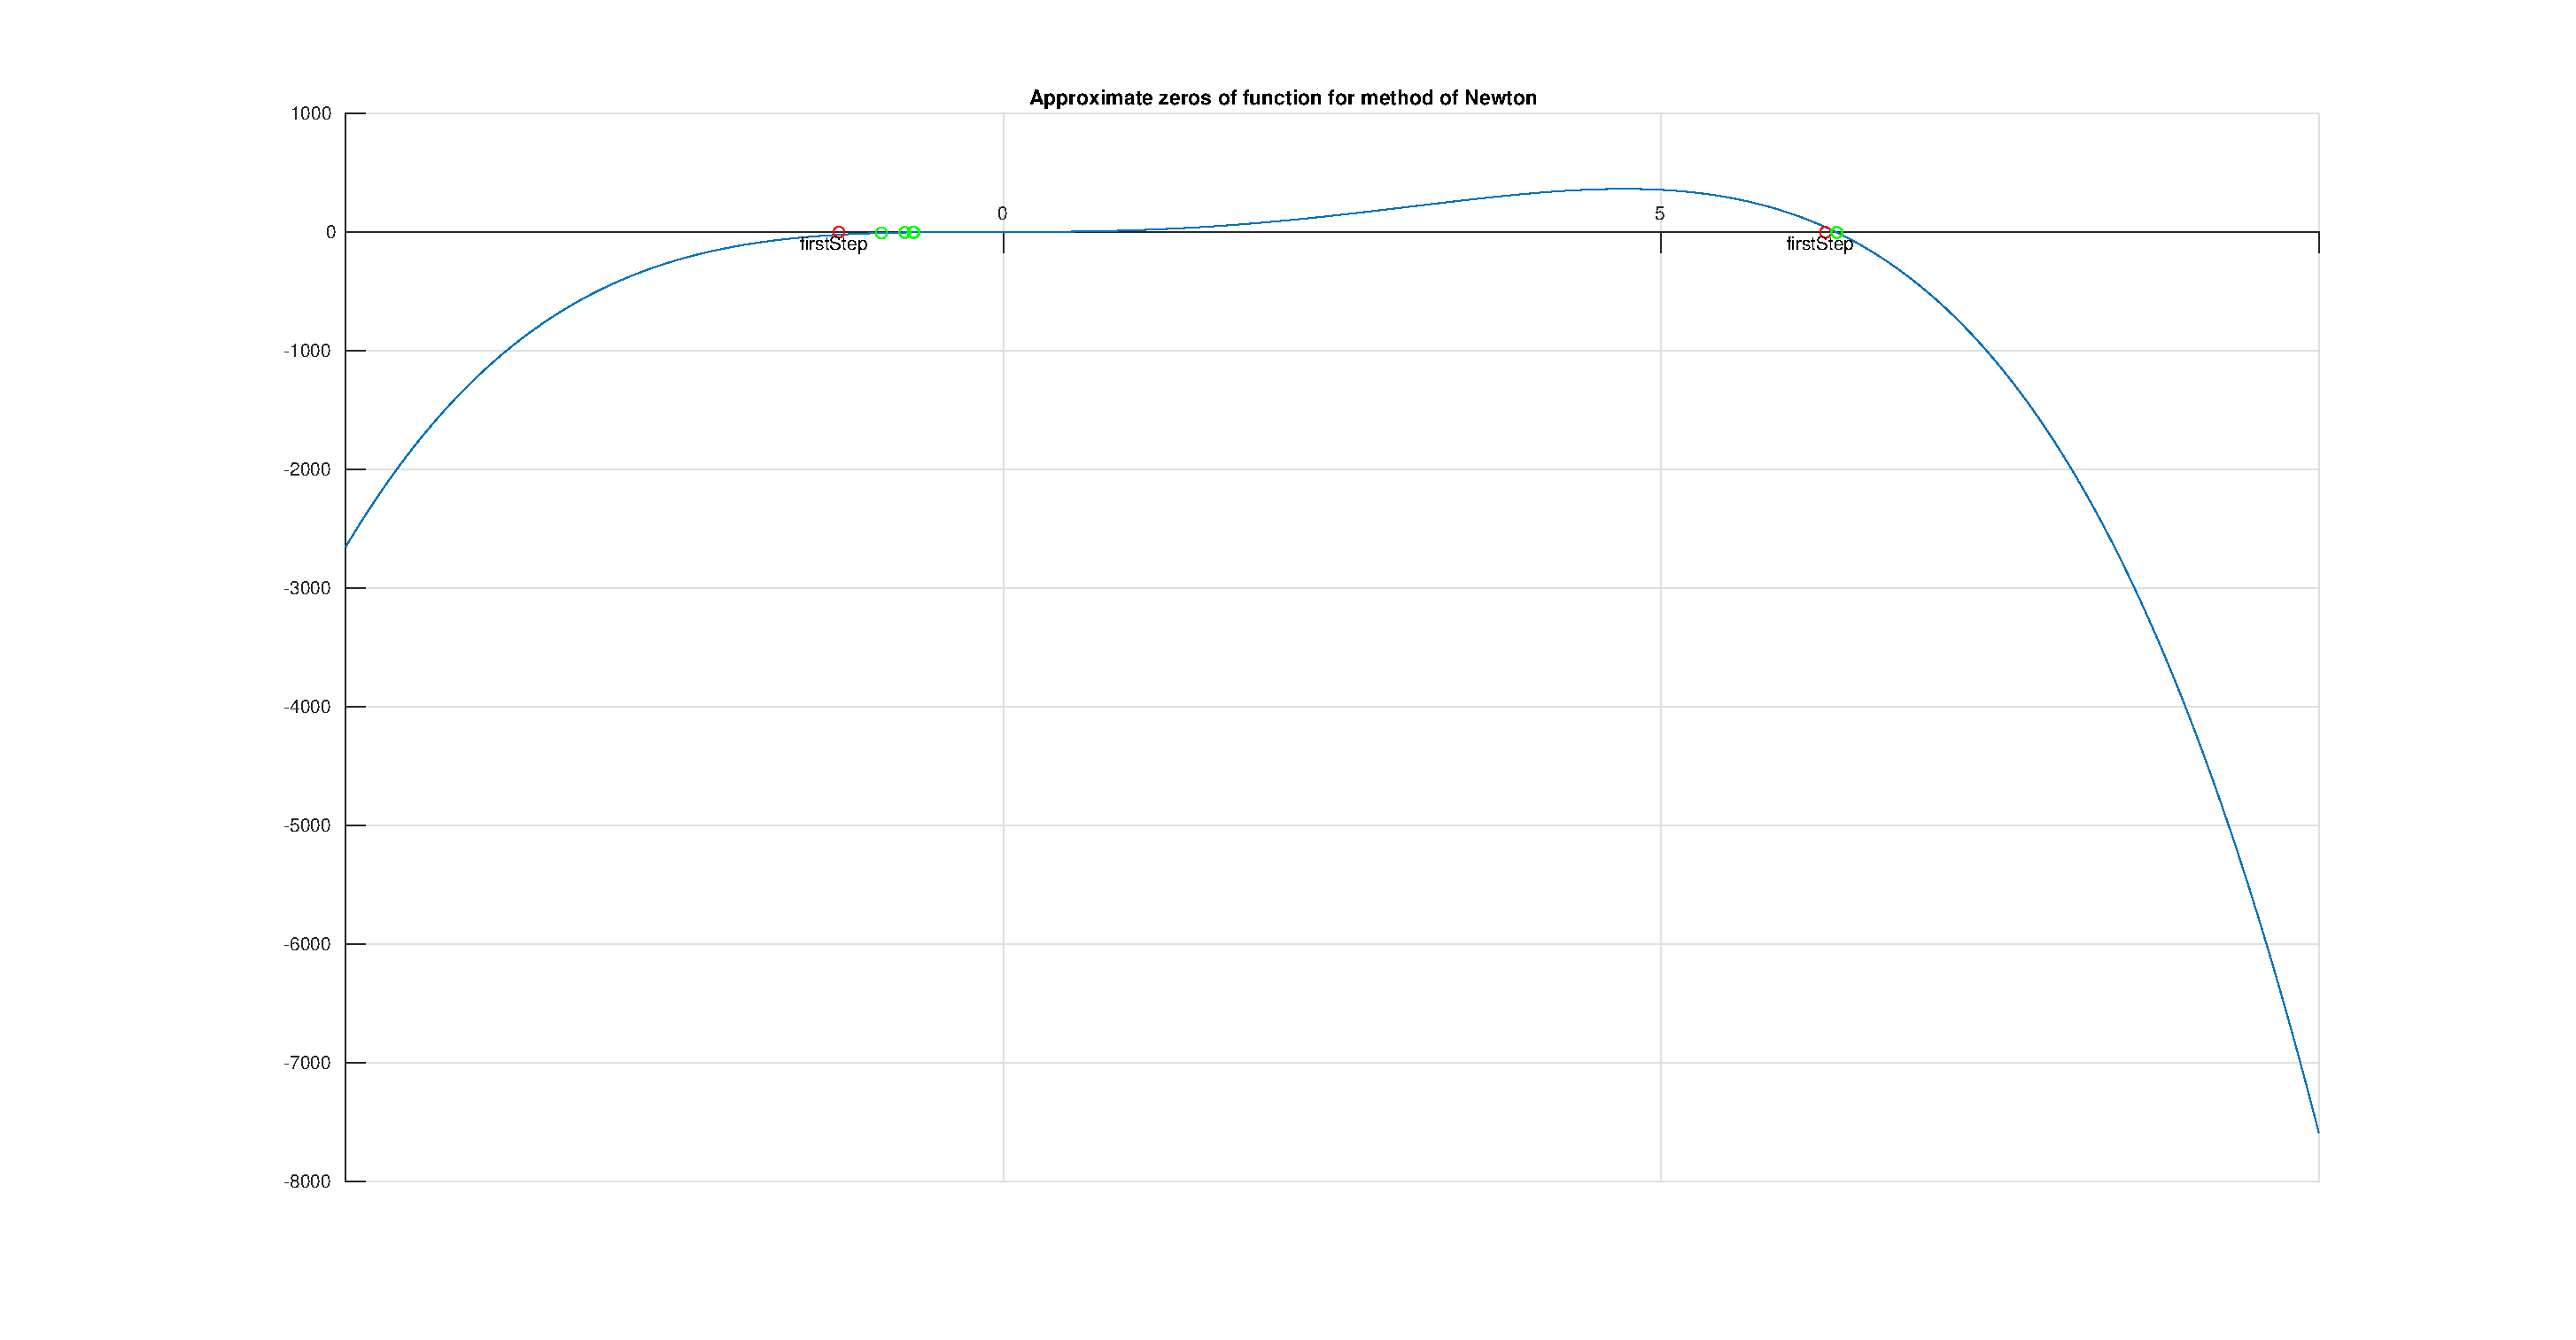
\includegraphics[scale=0.25]{task2newtonoverall.eps}
\end{center}

\begin{center}
   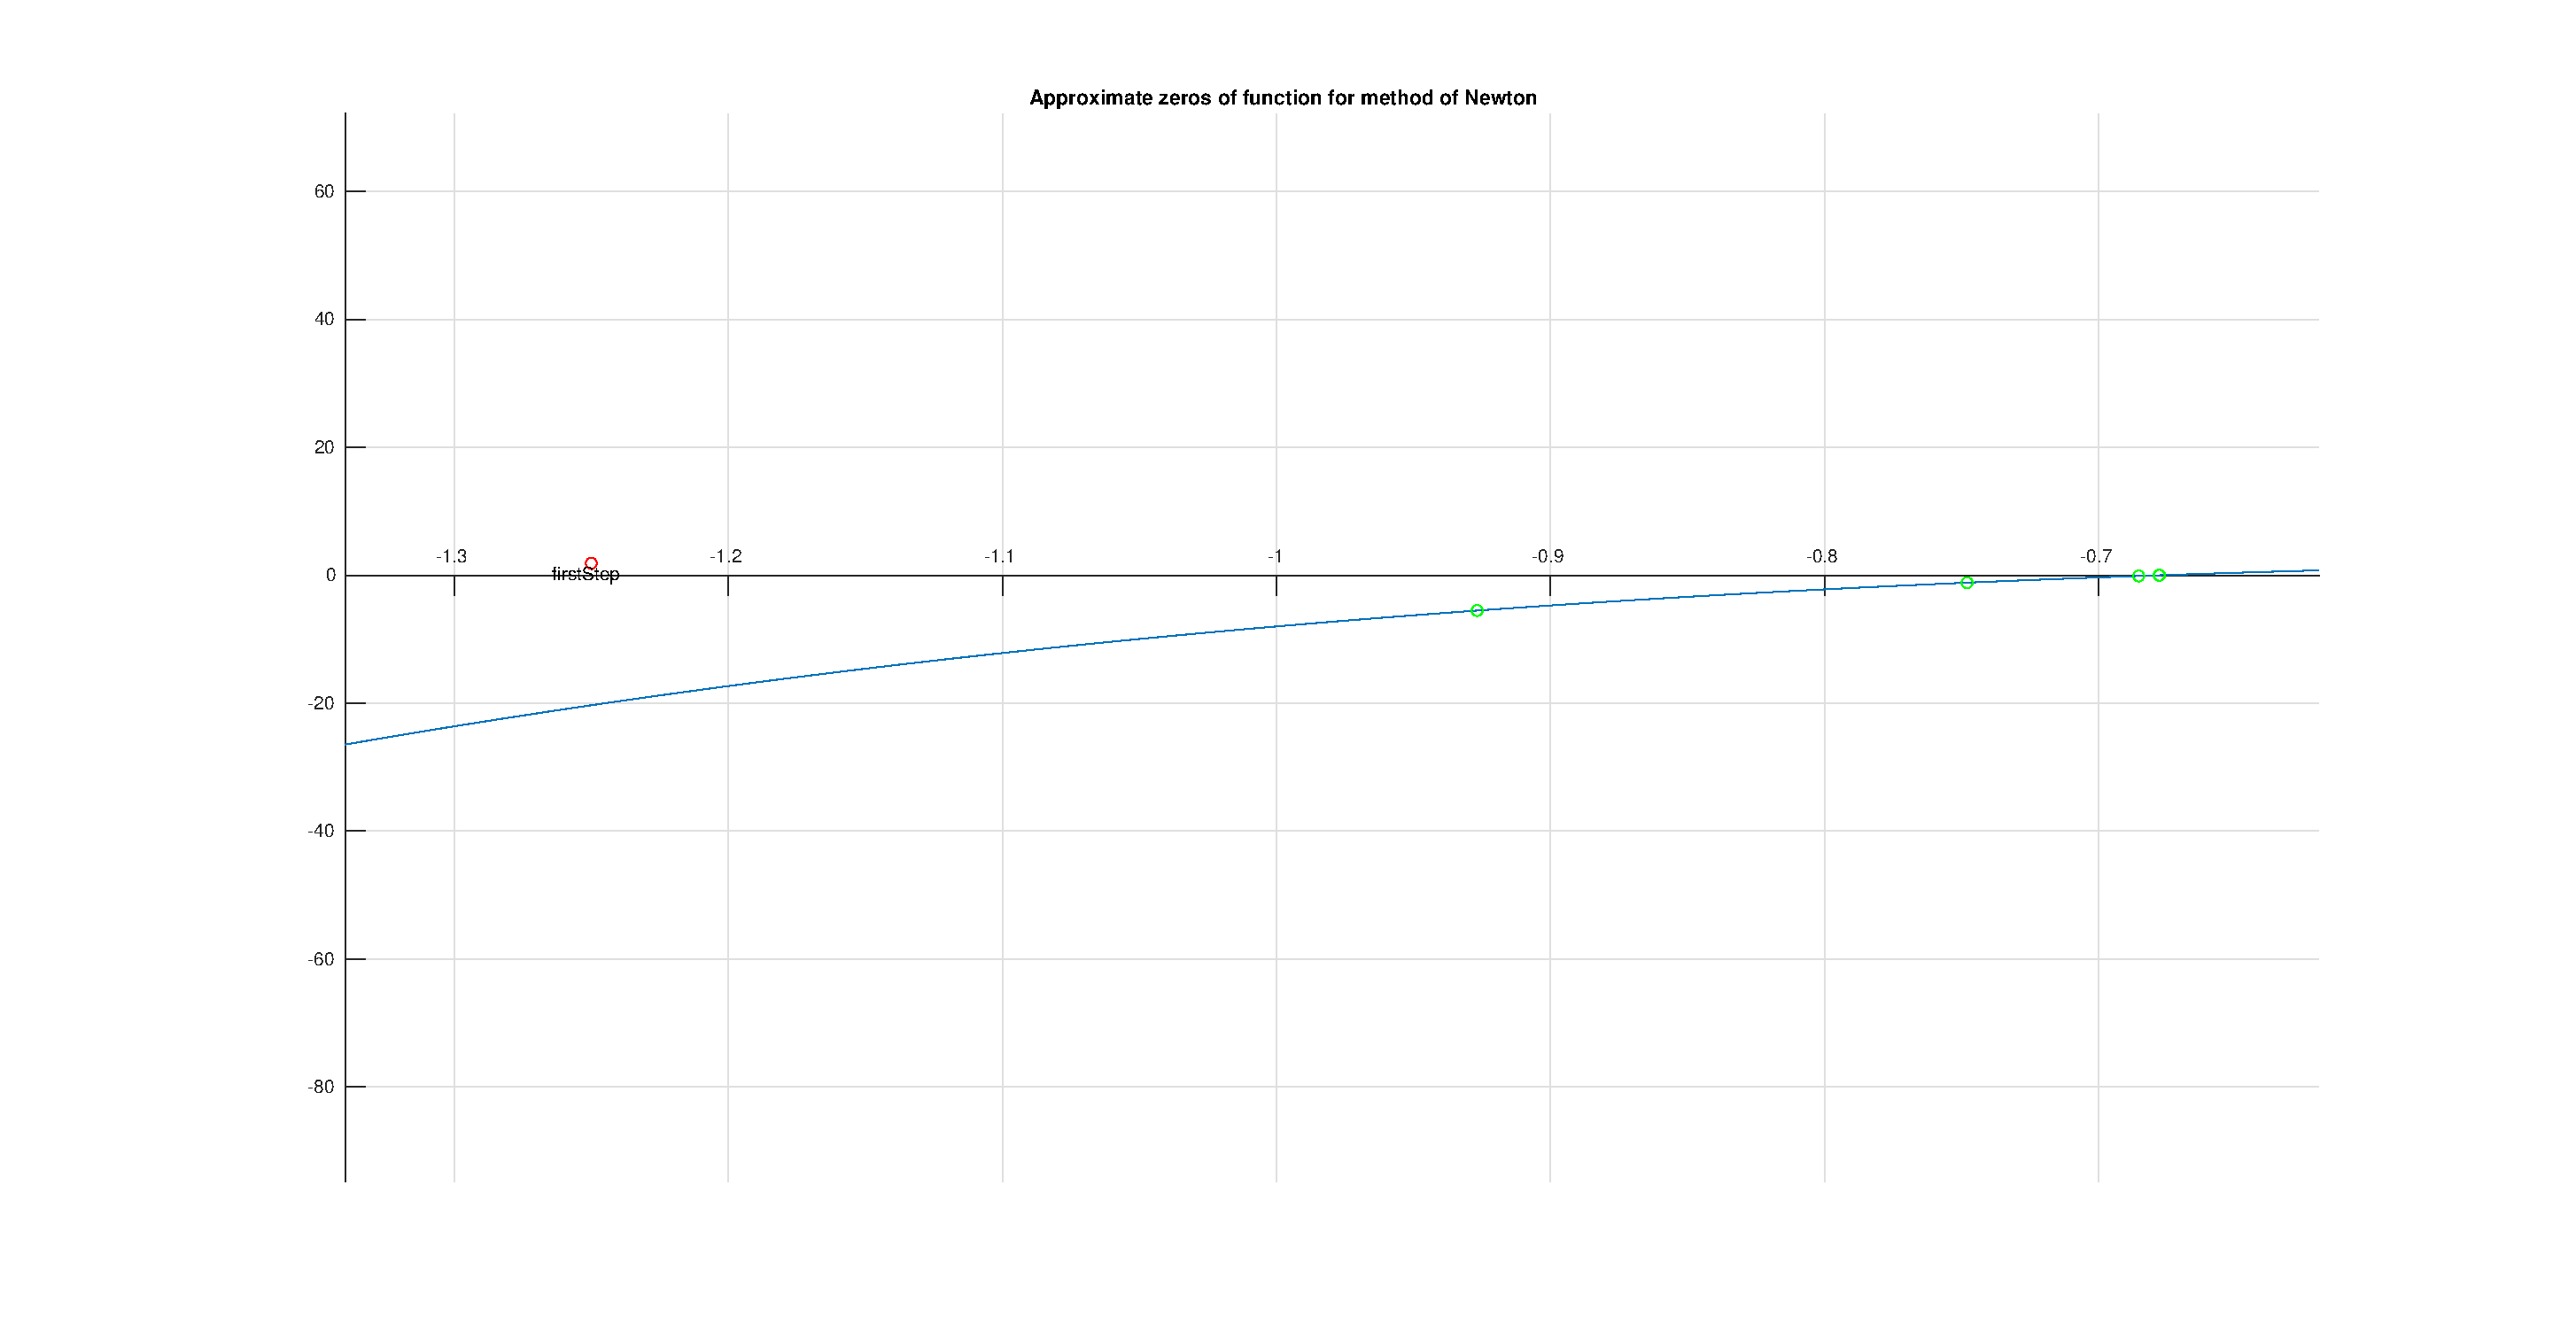
\includegraphics[scale=0.25]{task2newtonleft.eps}
\end{center}

\begin{center}
   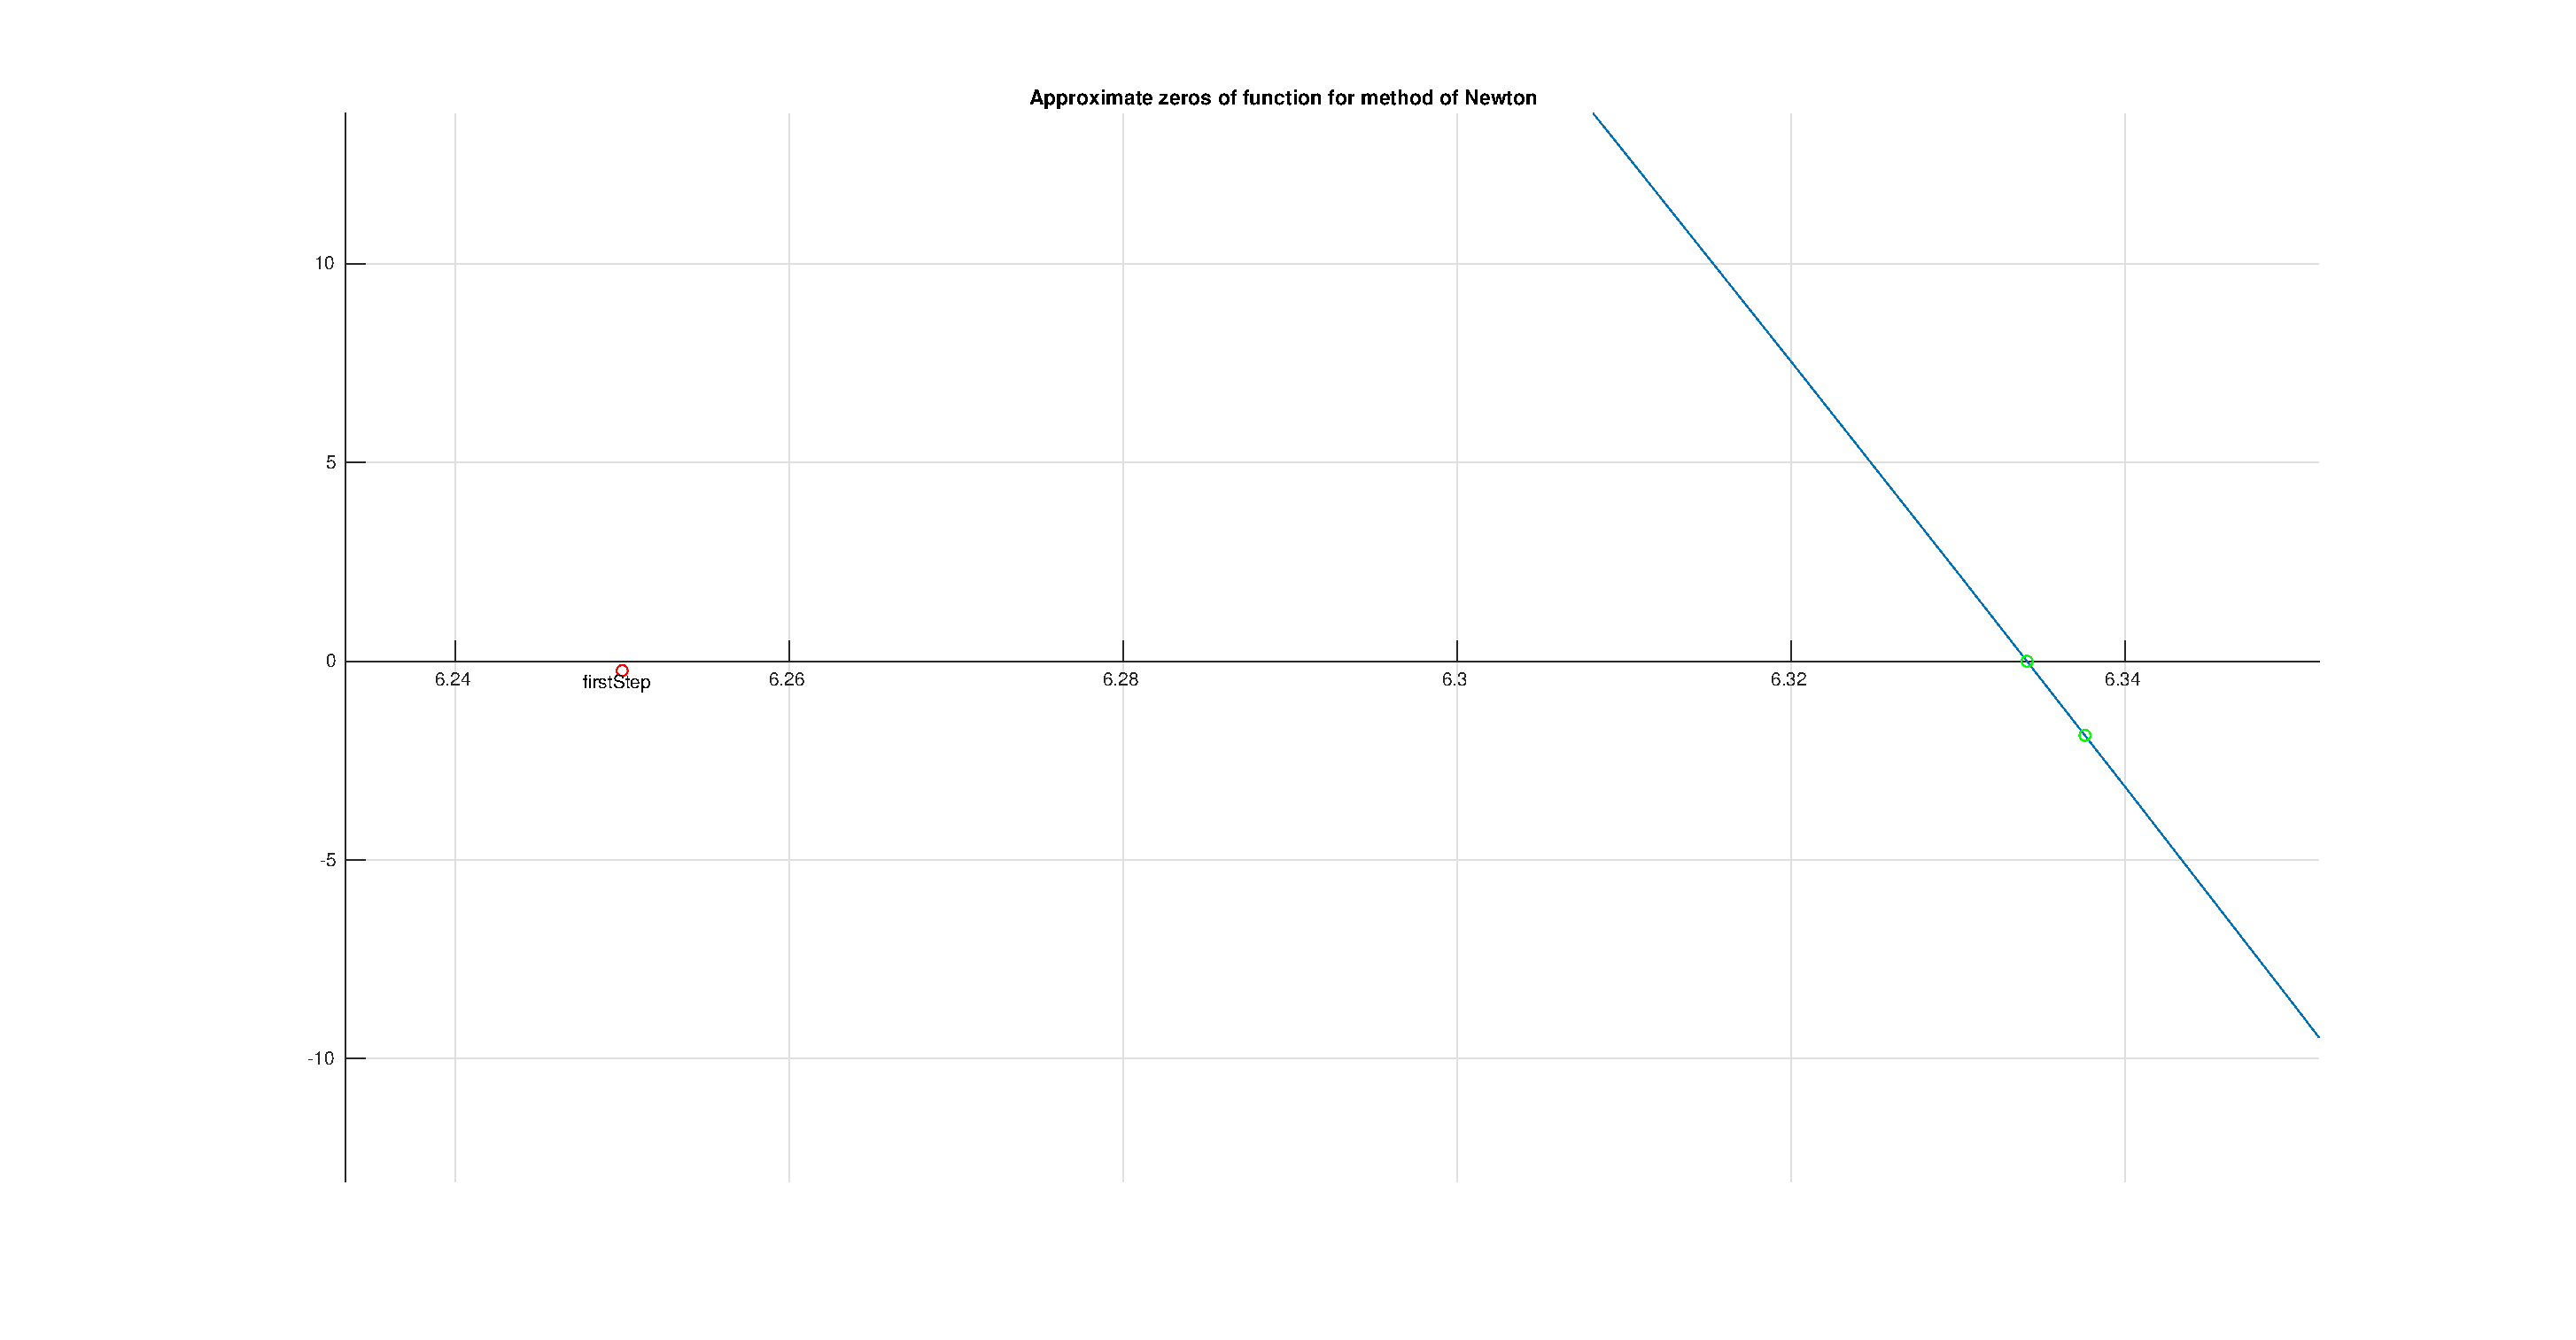
\includegraphics[scale=0.25]{task2newtonright.eps}
\end{center}


\begin{center}
  \begin{tabular}{| c  c c |}
\hline
Iteration & root         & f(root) \\
\hline
 1  &       -1.25   &       1.8879 \\
 \hline
 2  &    -0.92681  &         -5.52 \\
 \hline
 3  &   -0.74804   &       -1.159 \\
 \hline
 4  &   -0.68543   &     -0.11186 \\
 \hline
 5  &   -0.67797   &   -0.0014548 \\
 \hline
 6  &    -0.67787  &    -2.568e-07 \\
 \hline
 7  &   -0.67787   & -7.9936e-15 \\
 \hline
\end{tabular}
\end{center}

\begin{center}
  \begin{tabular}{| c  c c |}
\hline
Iteration & root         & f(root) \\
\hline
 1   &     6.25   &     -0.23707 \\
 \hline
 2   &   6.3376   &      -1.8647 \\
 \hline
 3   &  6.3341    &  -0.0029912 \\
 \hline
 4   &   6.3341   & -7.7134e-09 \\
 \hline
 5   &   6.3341   &  -7.1942e-14 \\
 \hline
\end{tabular}
\end{center}

As we can see Newton method calculated real roots in around the same number of iterations as method MM1, it was slightly slower than MM2. Newton method had pretty good accuracy, comparable to MM1 accuracy.


\chapter{Find real and complex roots of the polynomial using Laguerre's method}

\section{Problem}
We have to find all (real and complex) roots of the polynomial from previous exercise:
\[ f(x) = -2x^4+12x^3+4x^2+1x+3 \]
Using the Laguerre's method. Then we should compare those results with the MM2 version of the  M{\"u}ller's method.


\section{Theoretical Introduction}
Laguerre's method is defined by a single formula:

\[ x_{k+1} = x_k - \frac{nf(x_k)}{f^{'}(x_k) \pm \sqrt{(n-1)[(n-1)( (f^{'}(x_k))^2 - nf(x_k)f^{''}(x_k) )]}} \]
Where:
$n$ - order of the polynomial

This formula is similar to the one from MM2 but also takes order of the polynomial into consideration. In general this method is better. For polynomials with real roots it is globally convergent. It does not have formal analysis for complex roots but it usually shows good numerical properties, although divergence may happen.

\section{Results}

\begin{center}
   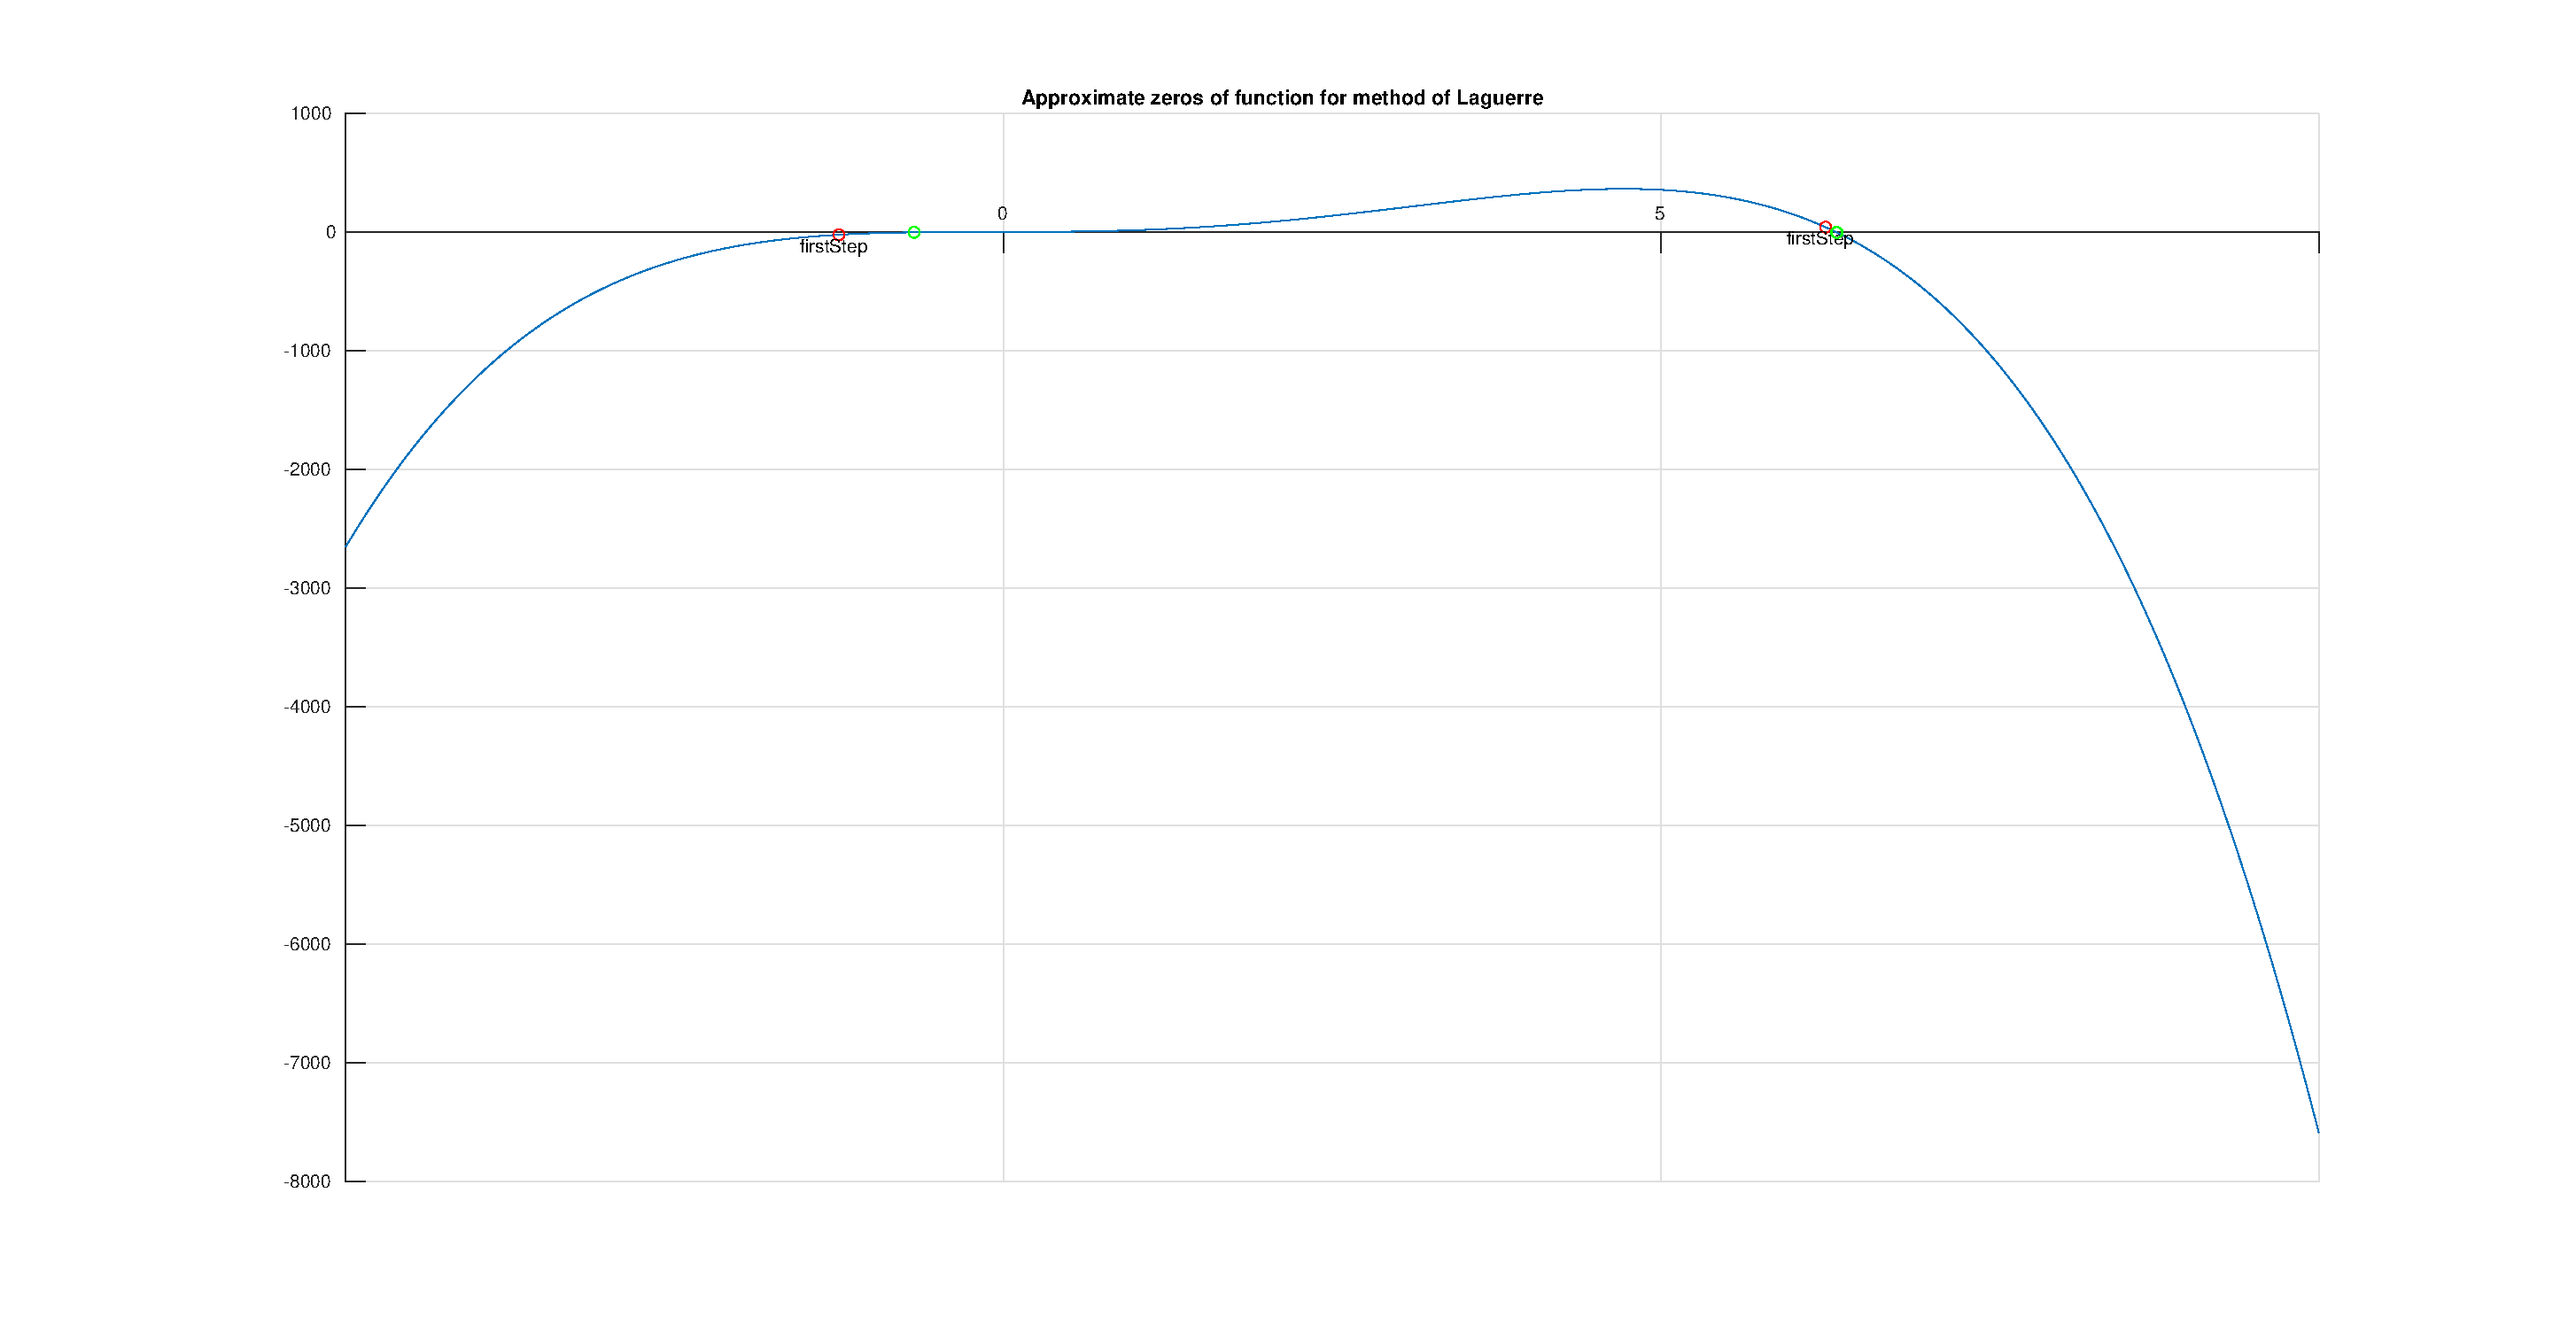
\includegraphics[scale=0.25]{task3overall.eps}
\end{center}


\begin{center}
   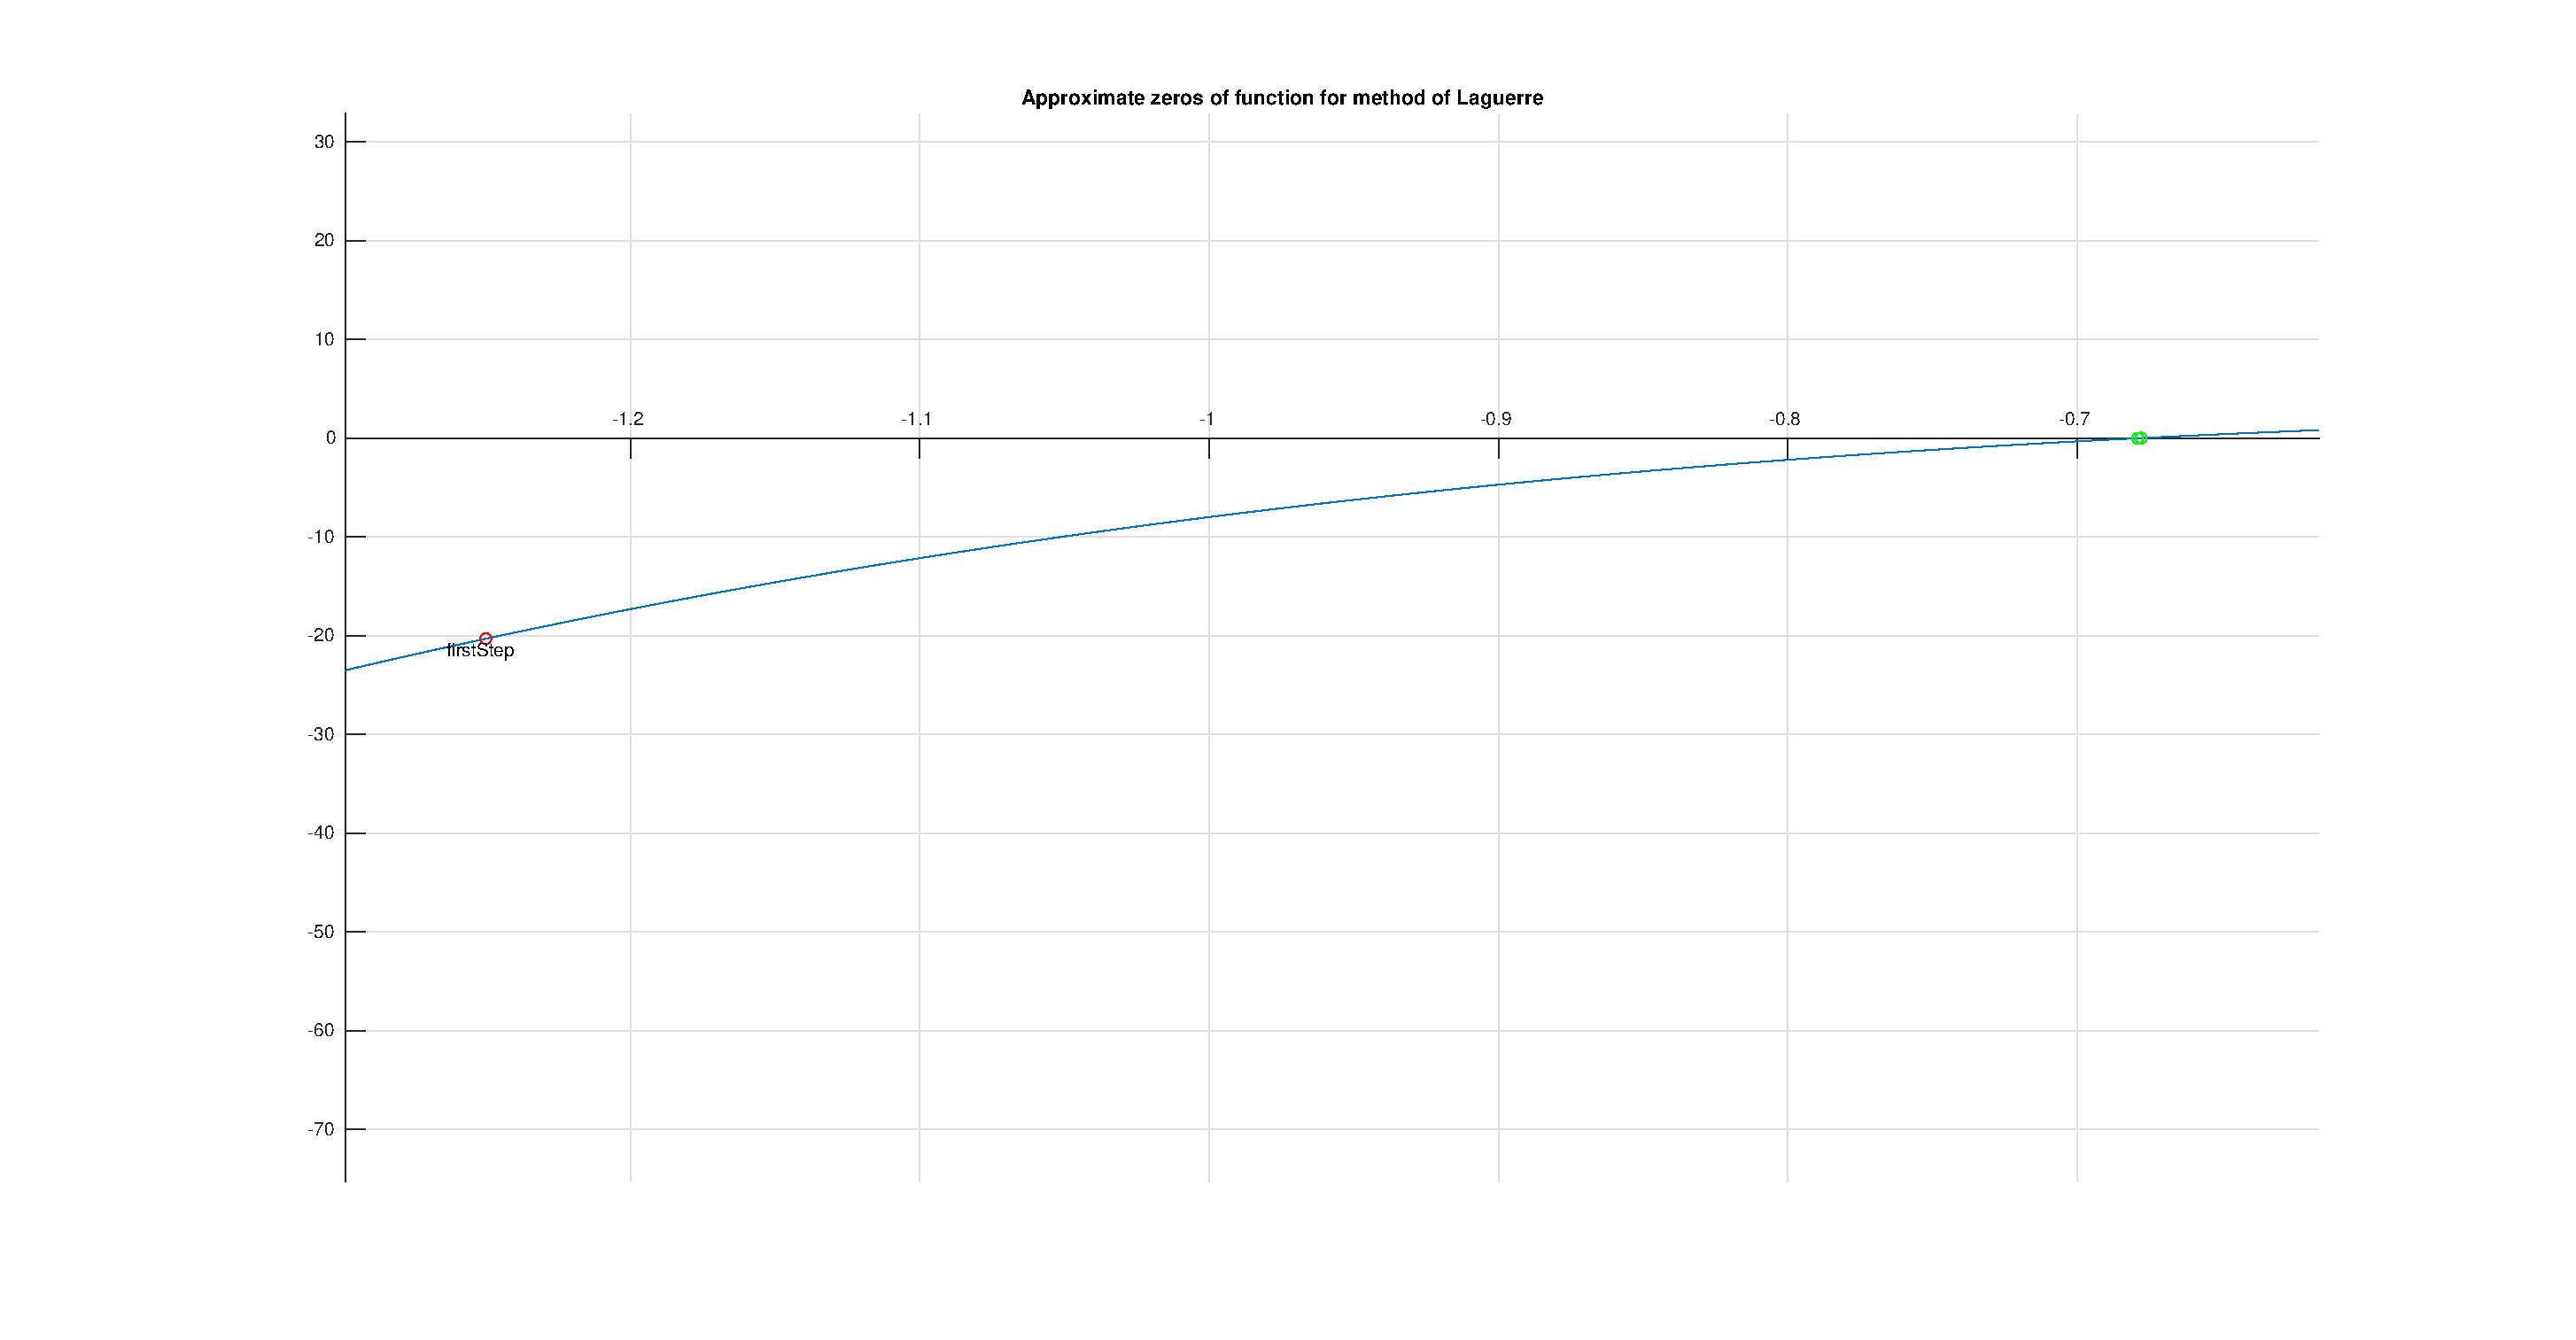
\includegraphics[scale=0.25]{task3left.eps}
\end{center}

\begin{center}
   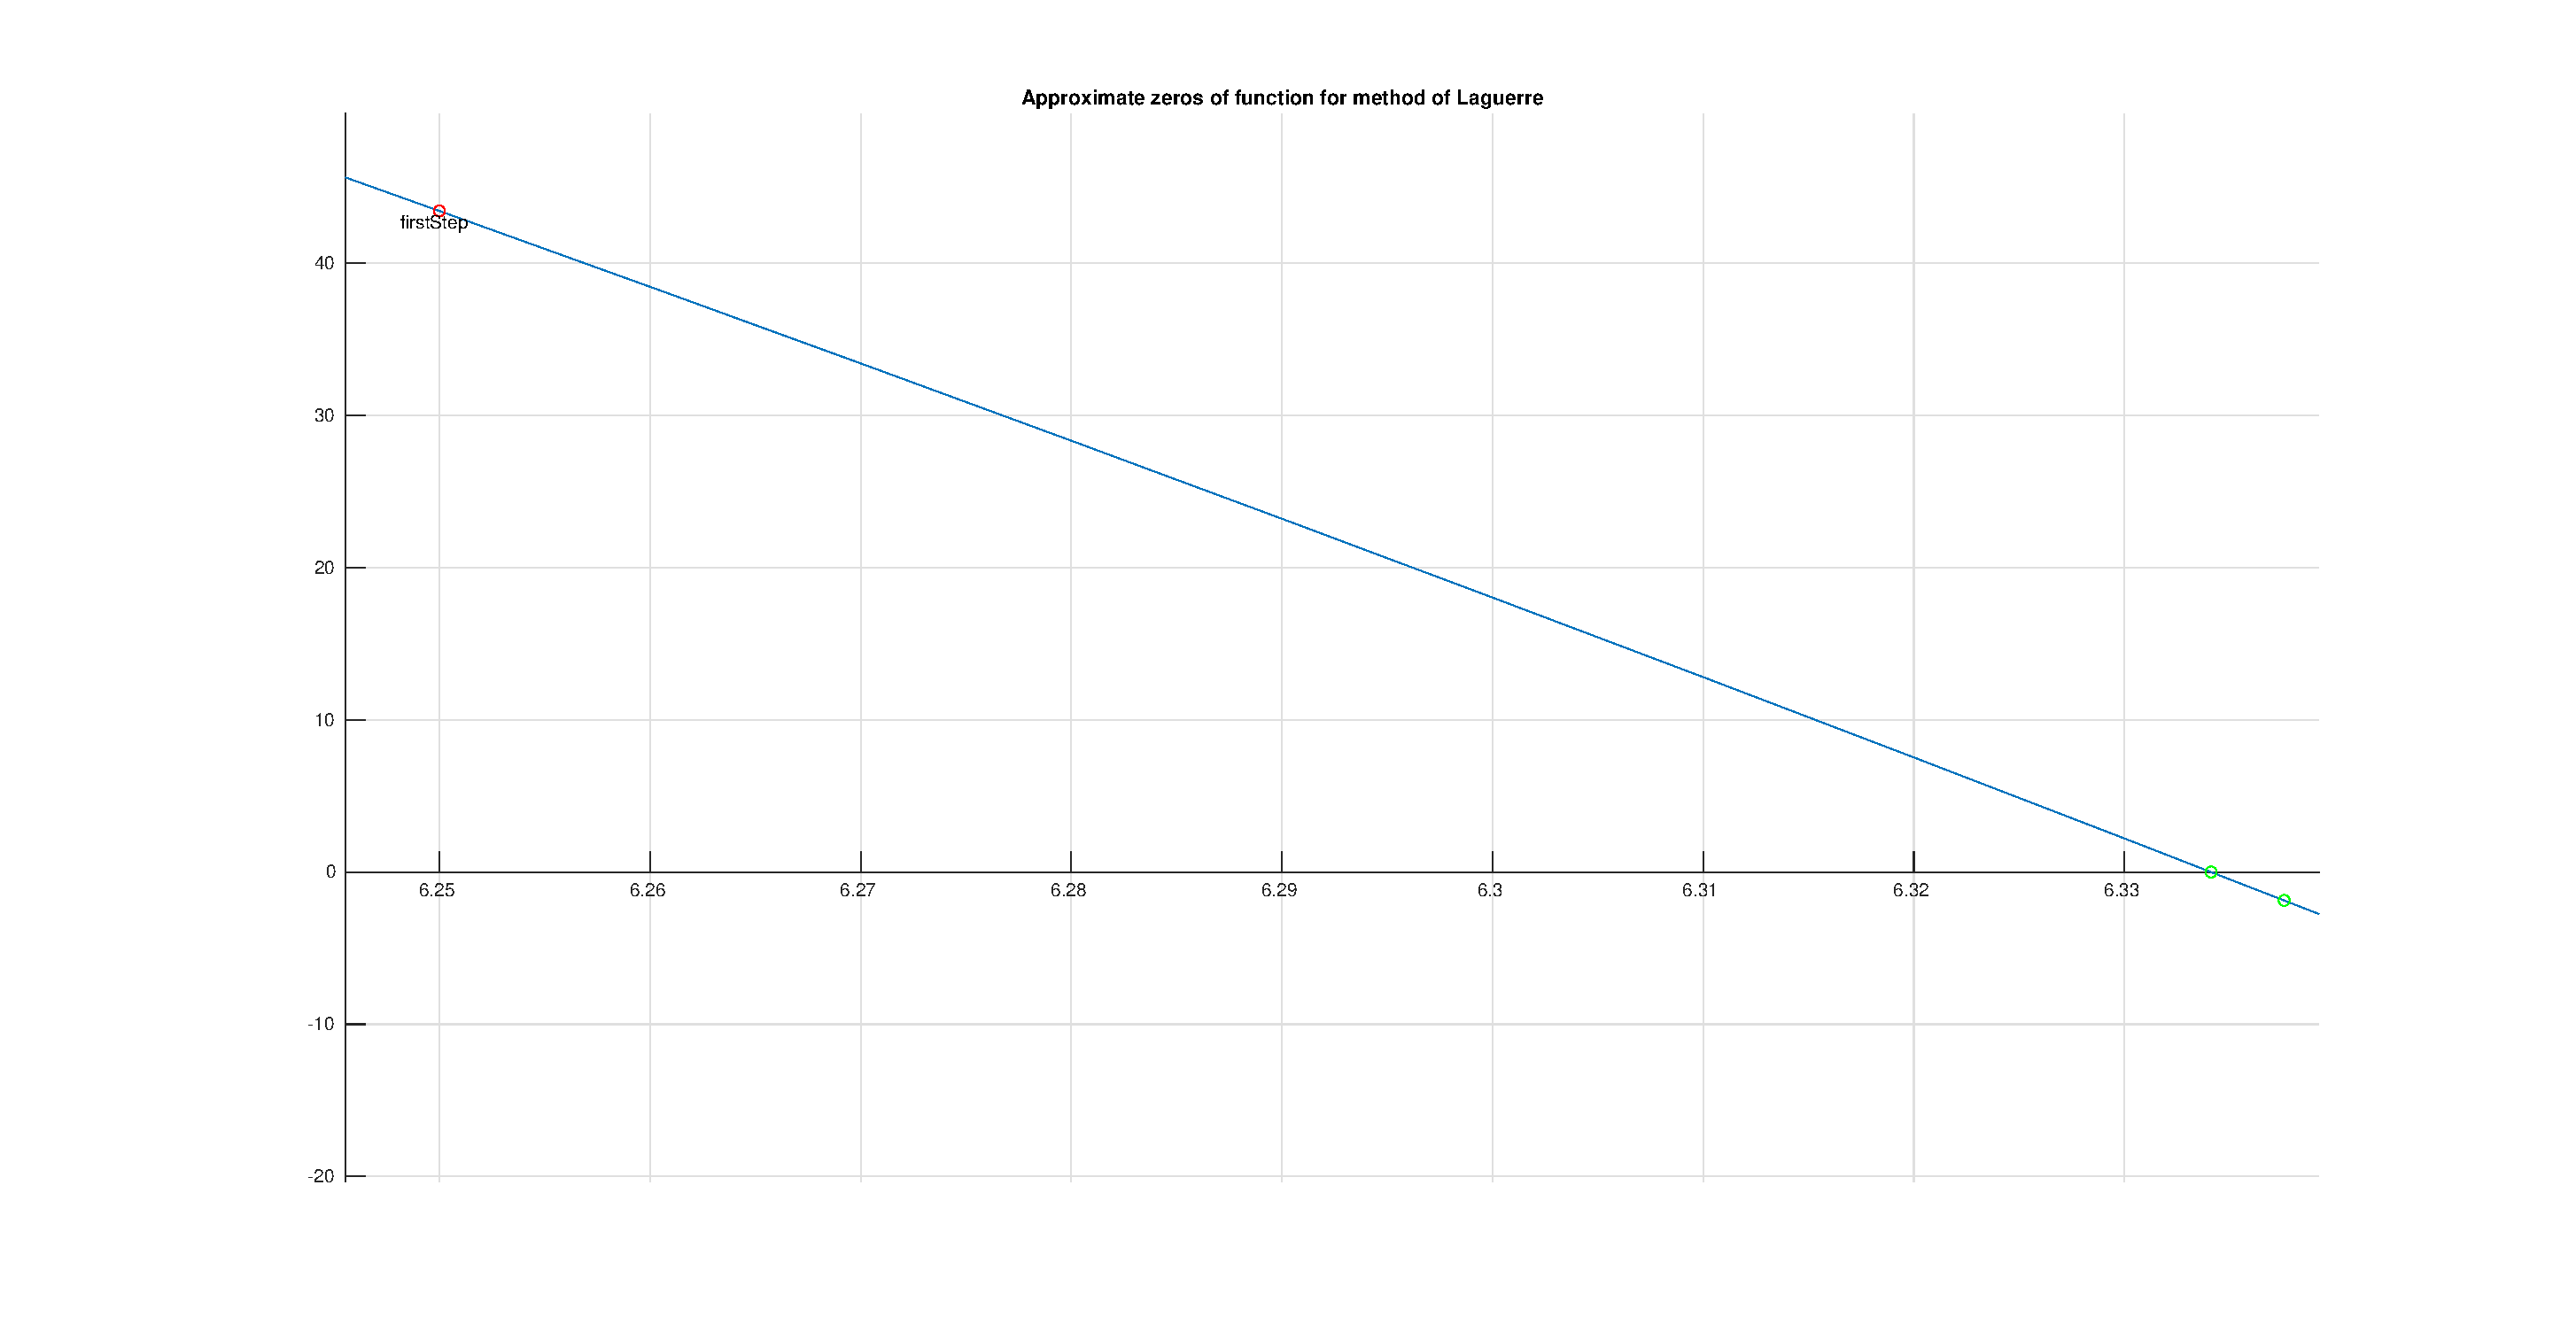
\includegraphics[scale=0.25]{task3right.eps}
\end{center}

\begin{center}
   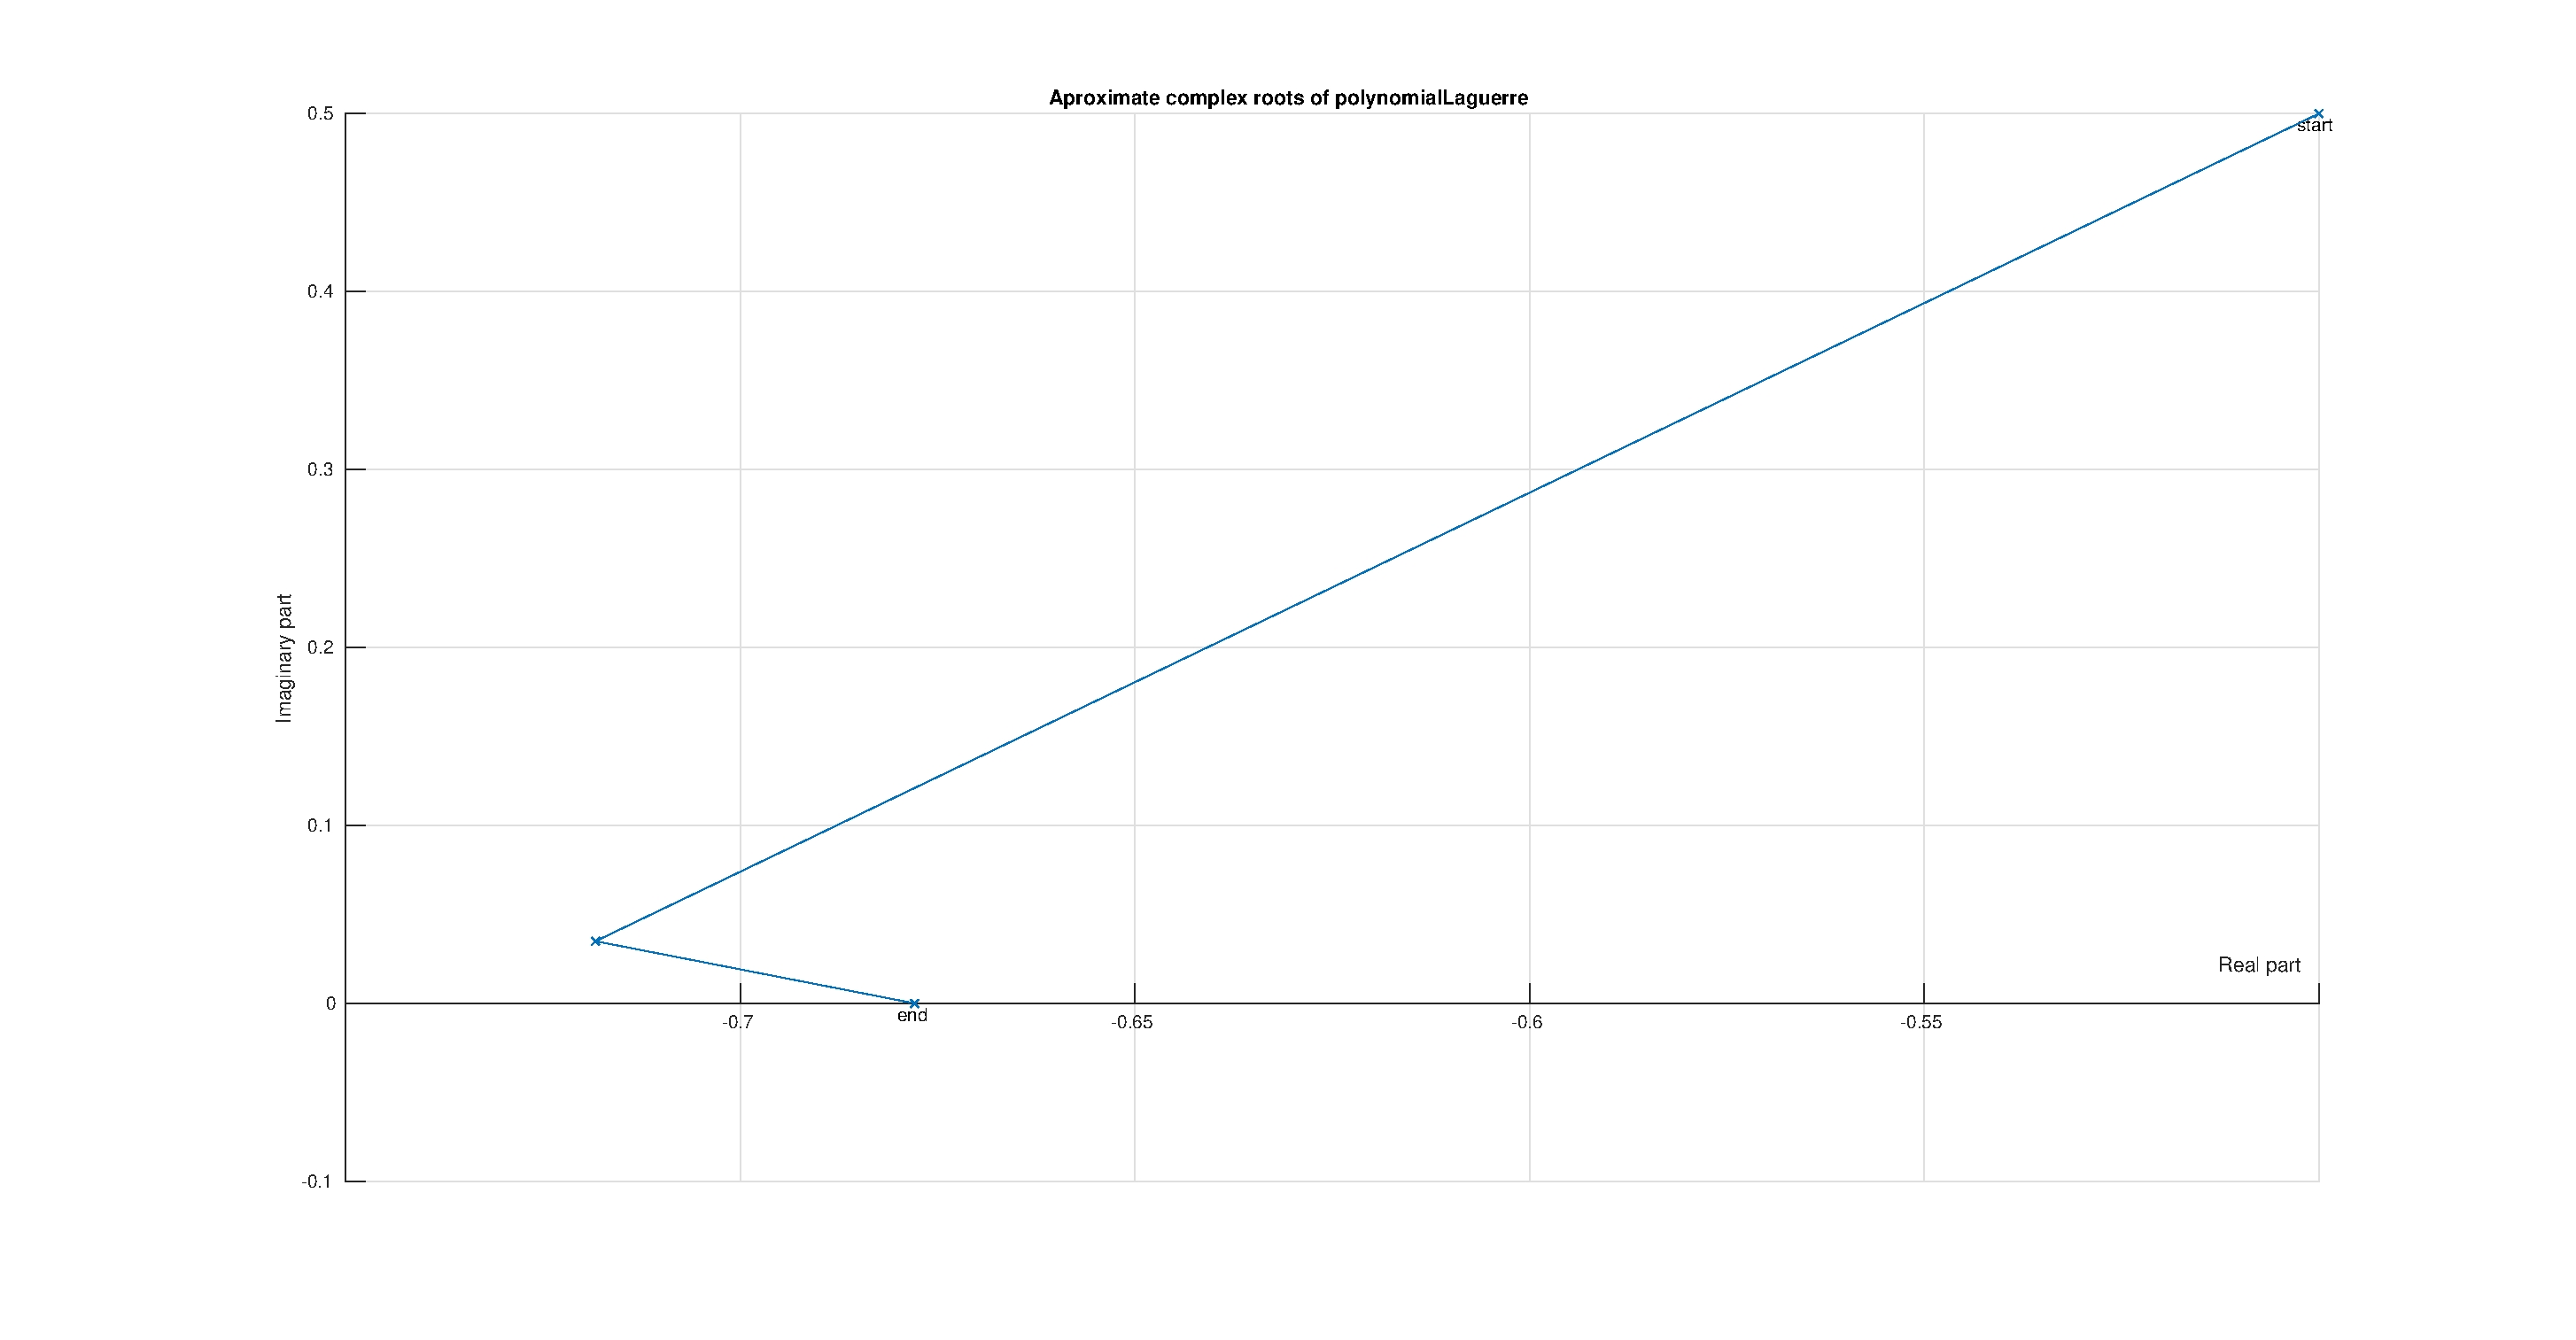
\includegraphics[scale=0.25]{task3complexoverall.eps}
\end{center}

\begin{center}
   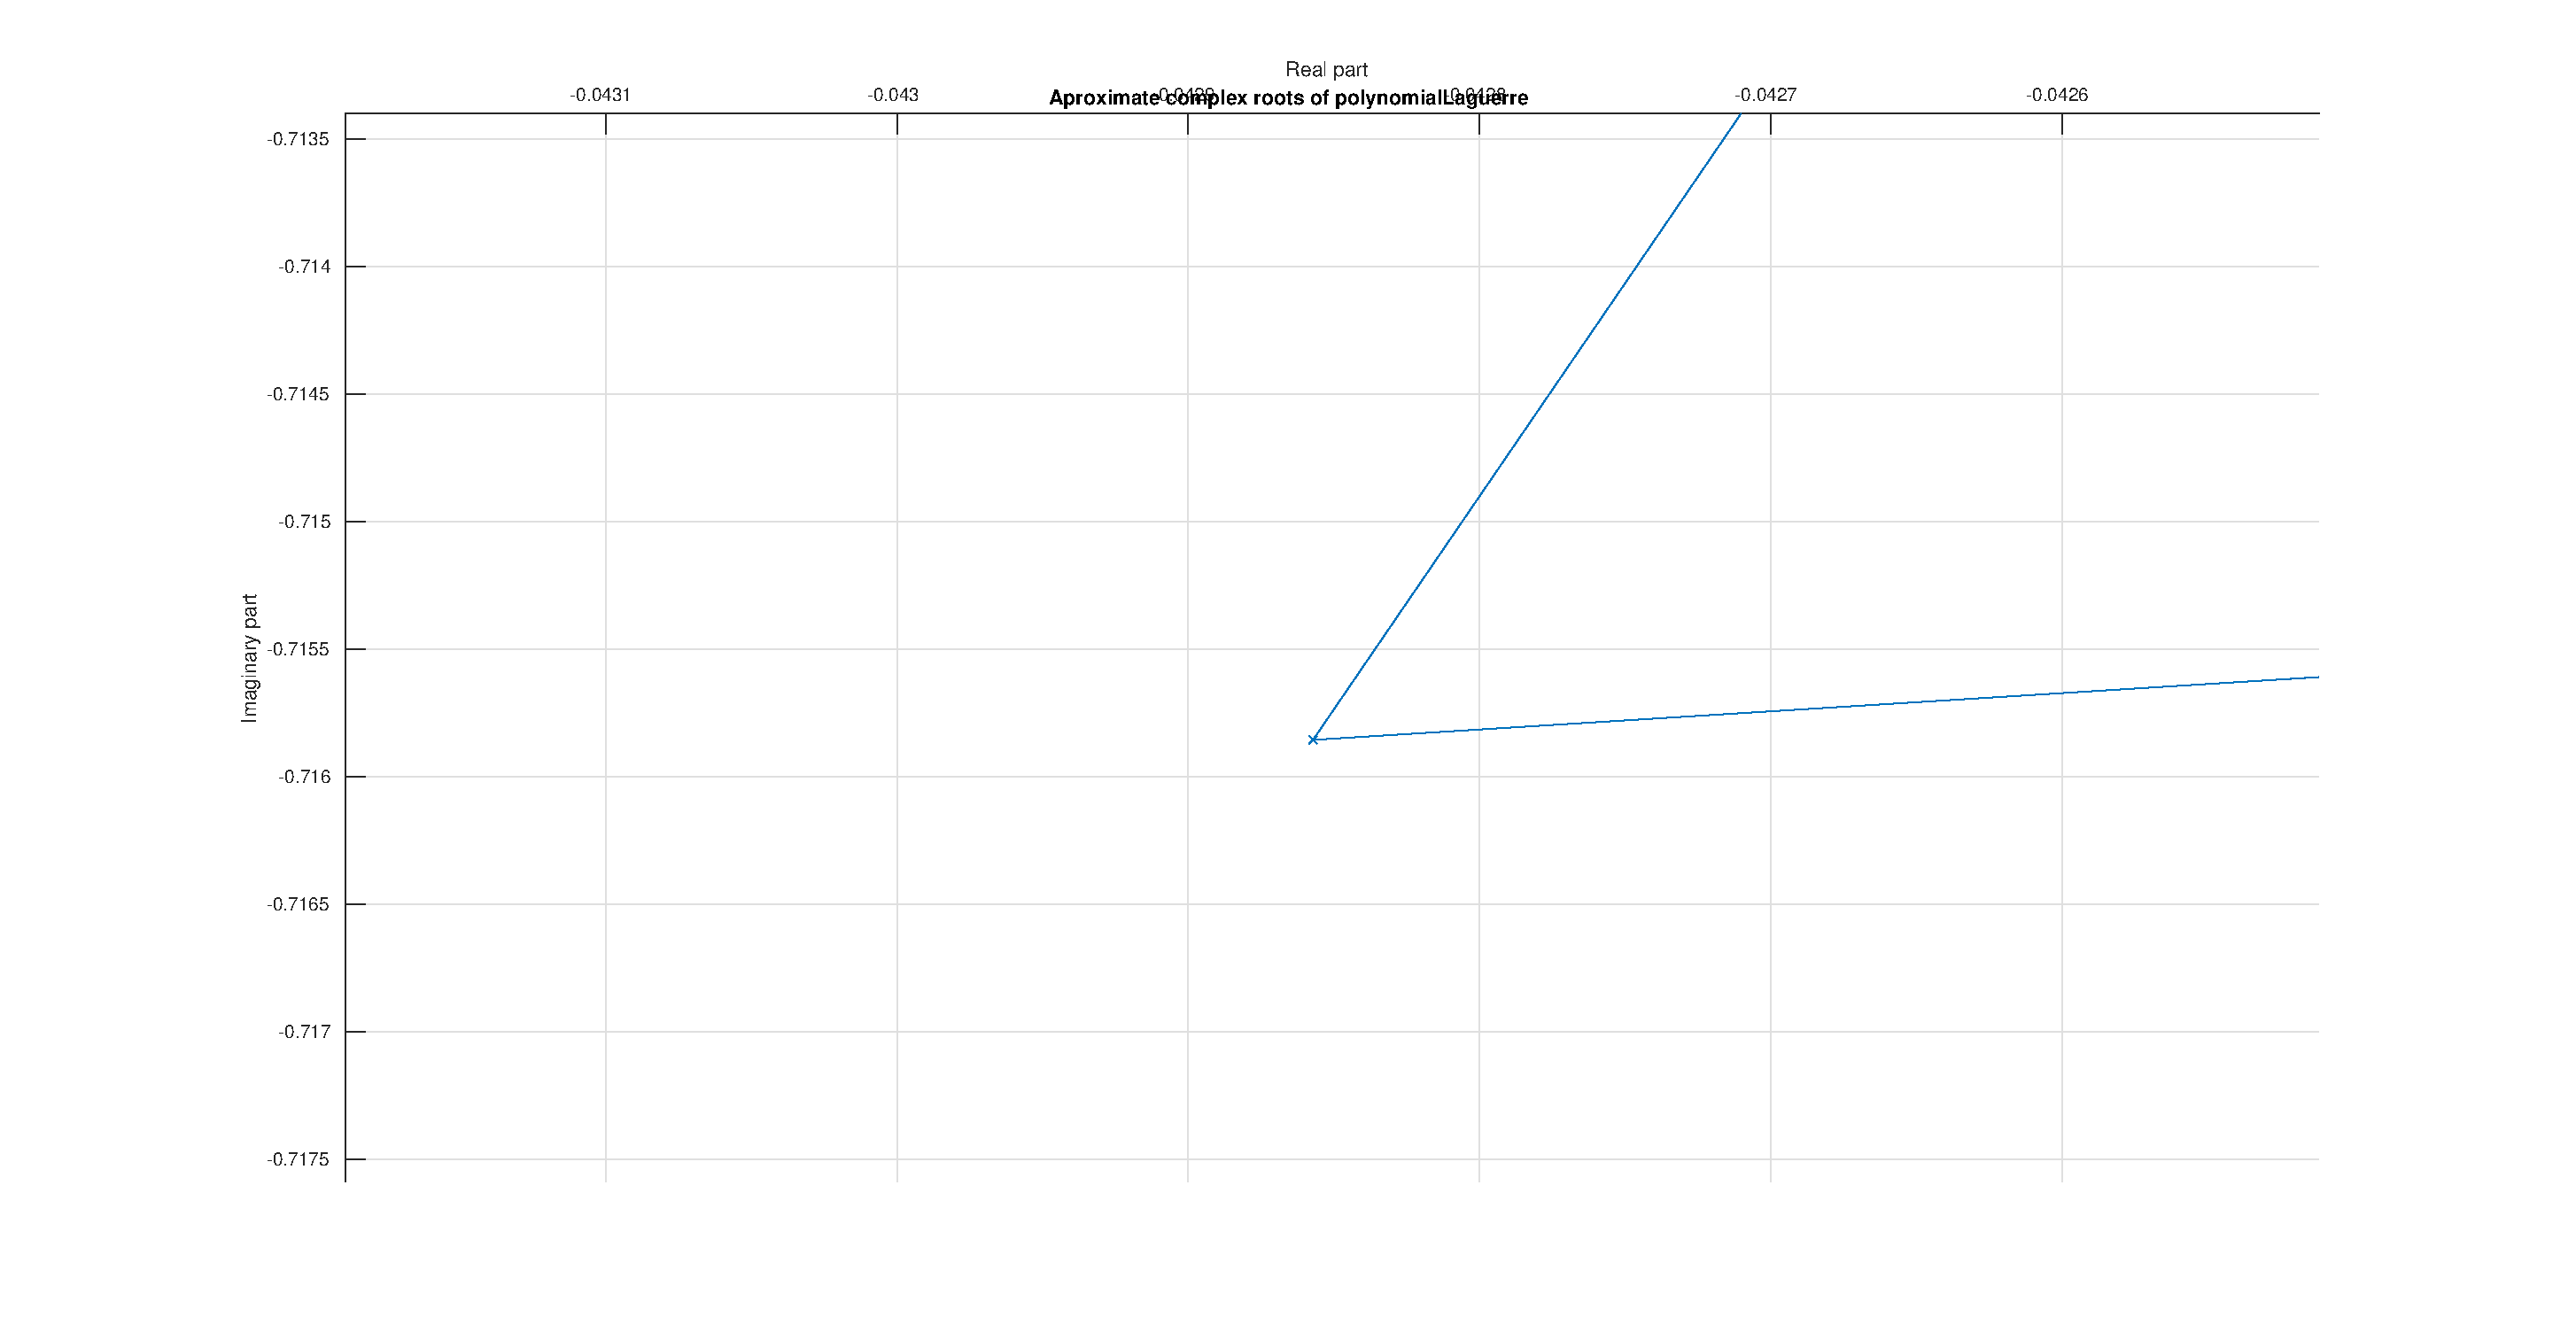
\includegraphics[scale=0.25]{task3complexleft.eps}
\end{center}

\begin{center}
   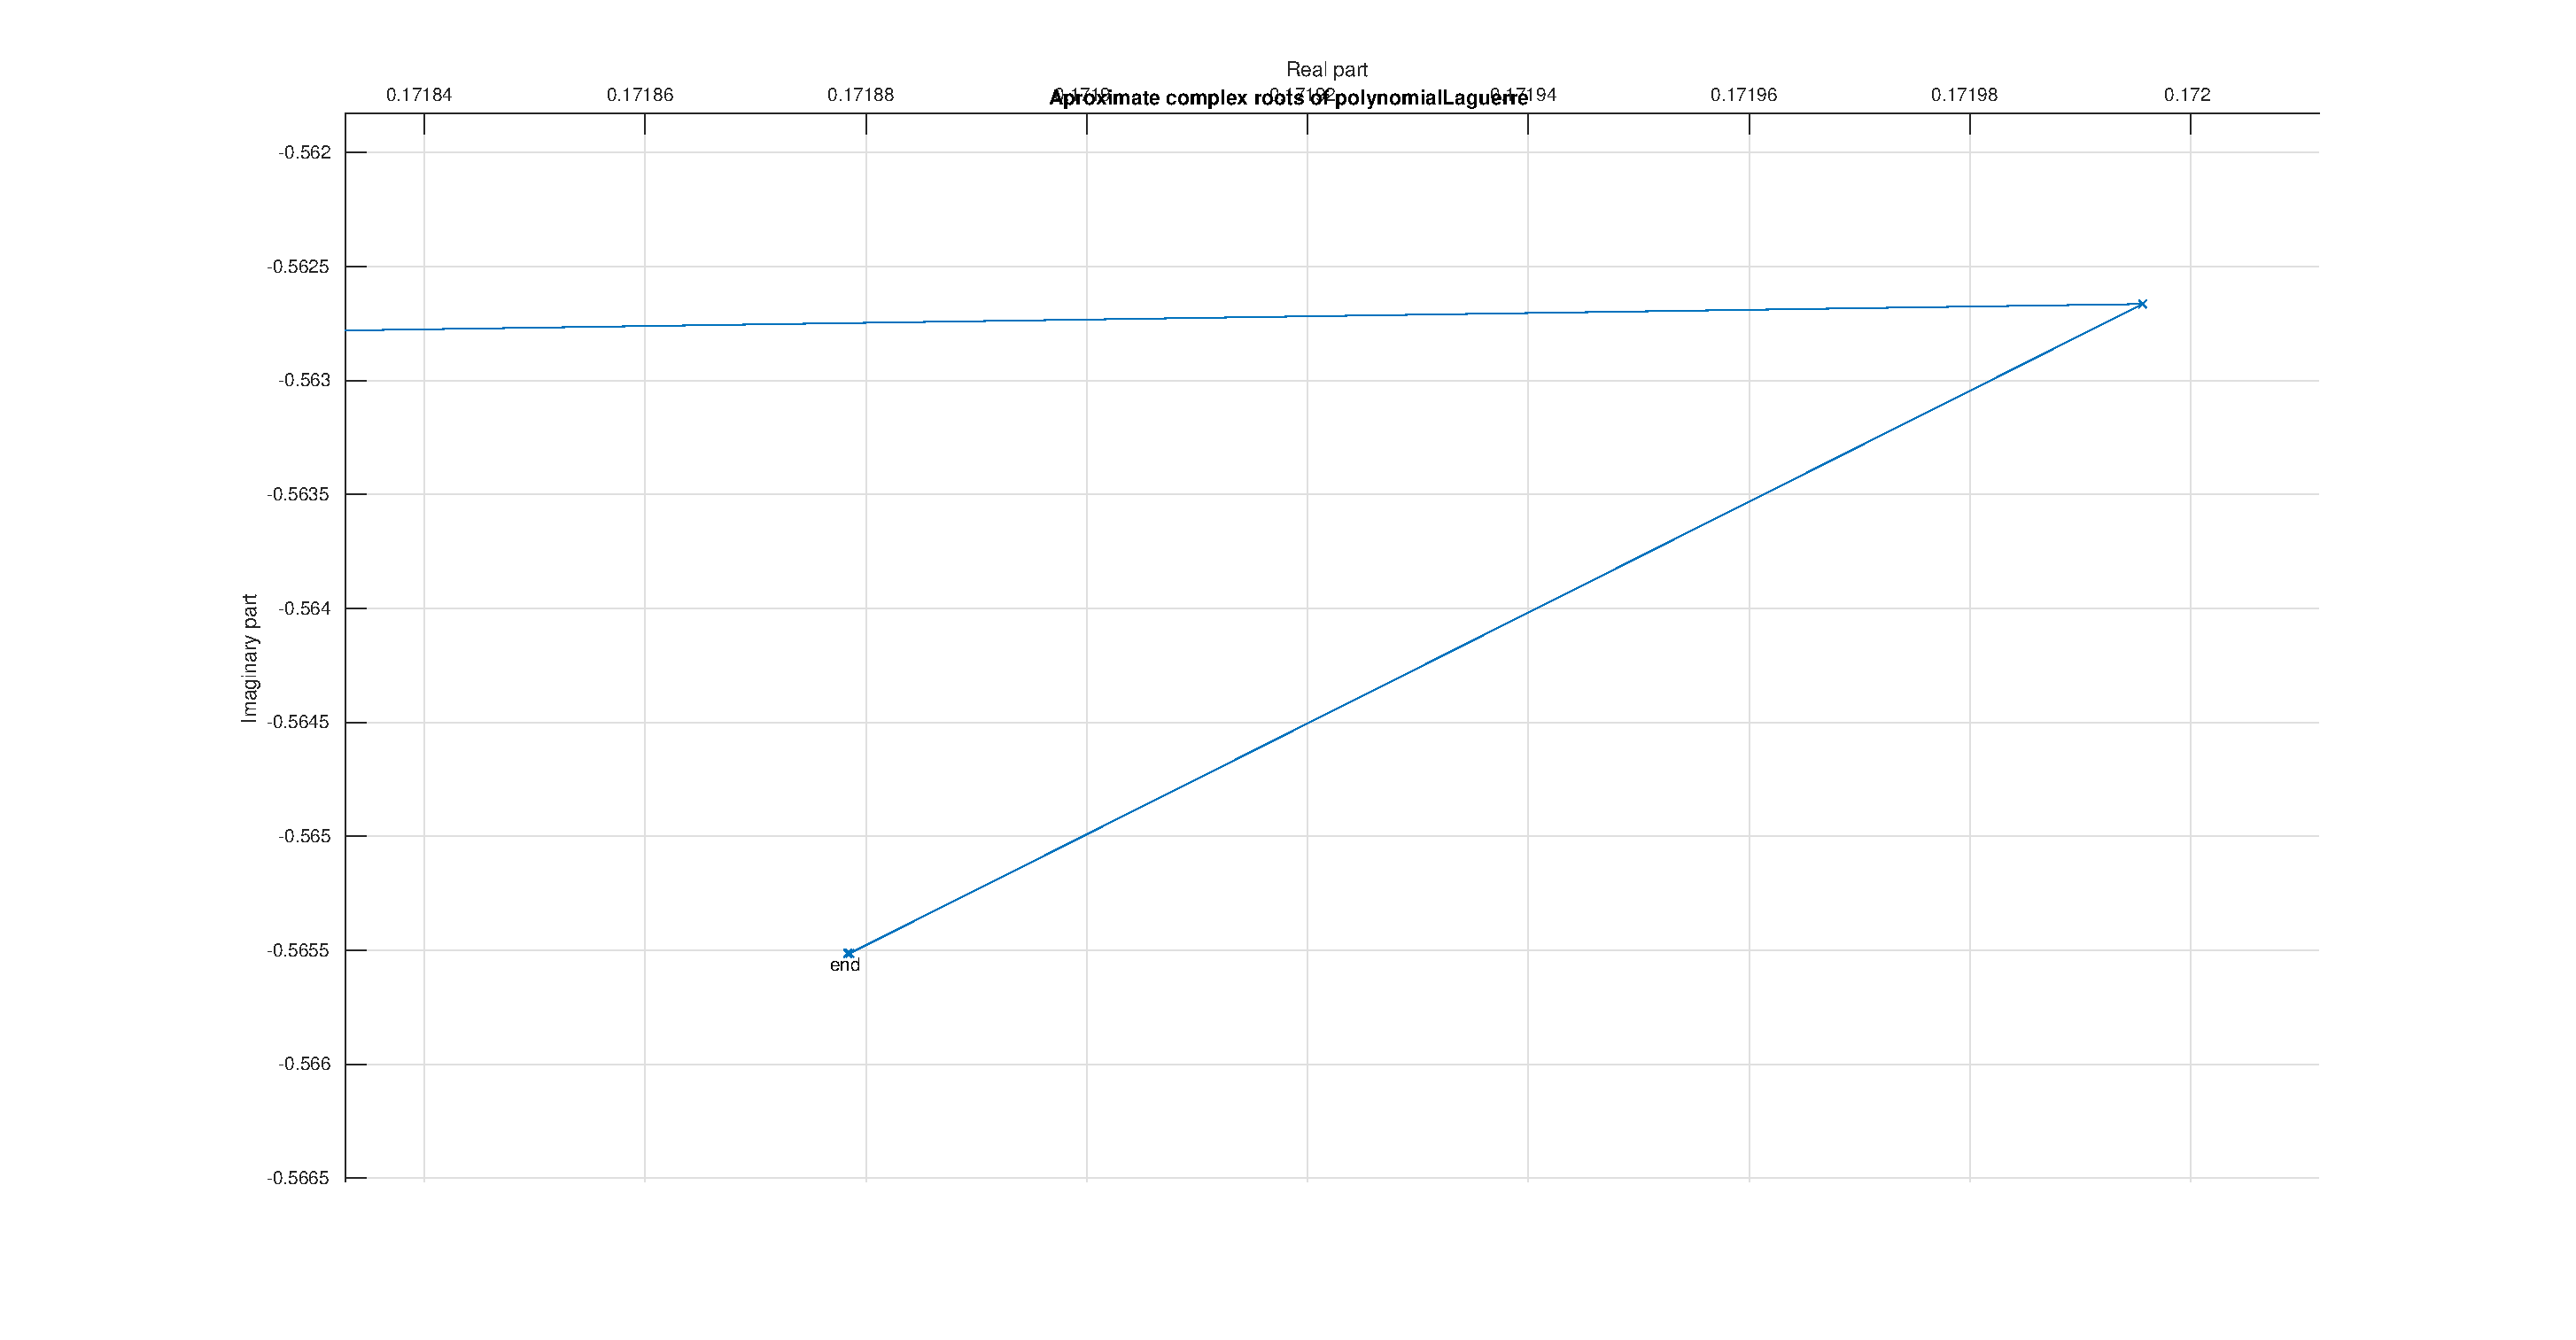
\includegraphics[scale=0.25]{task3complexright.eps}
\end{center}

\begin{center}
   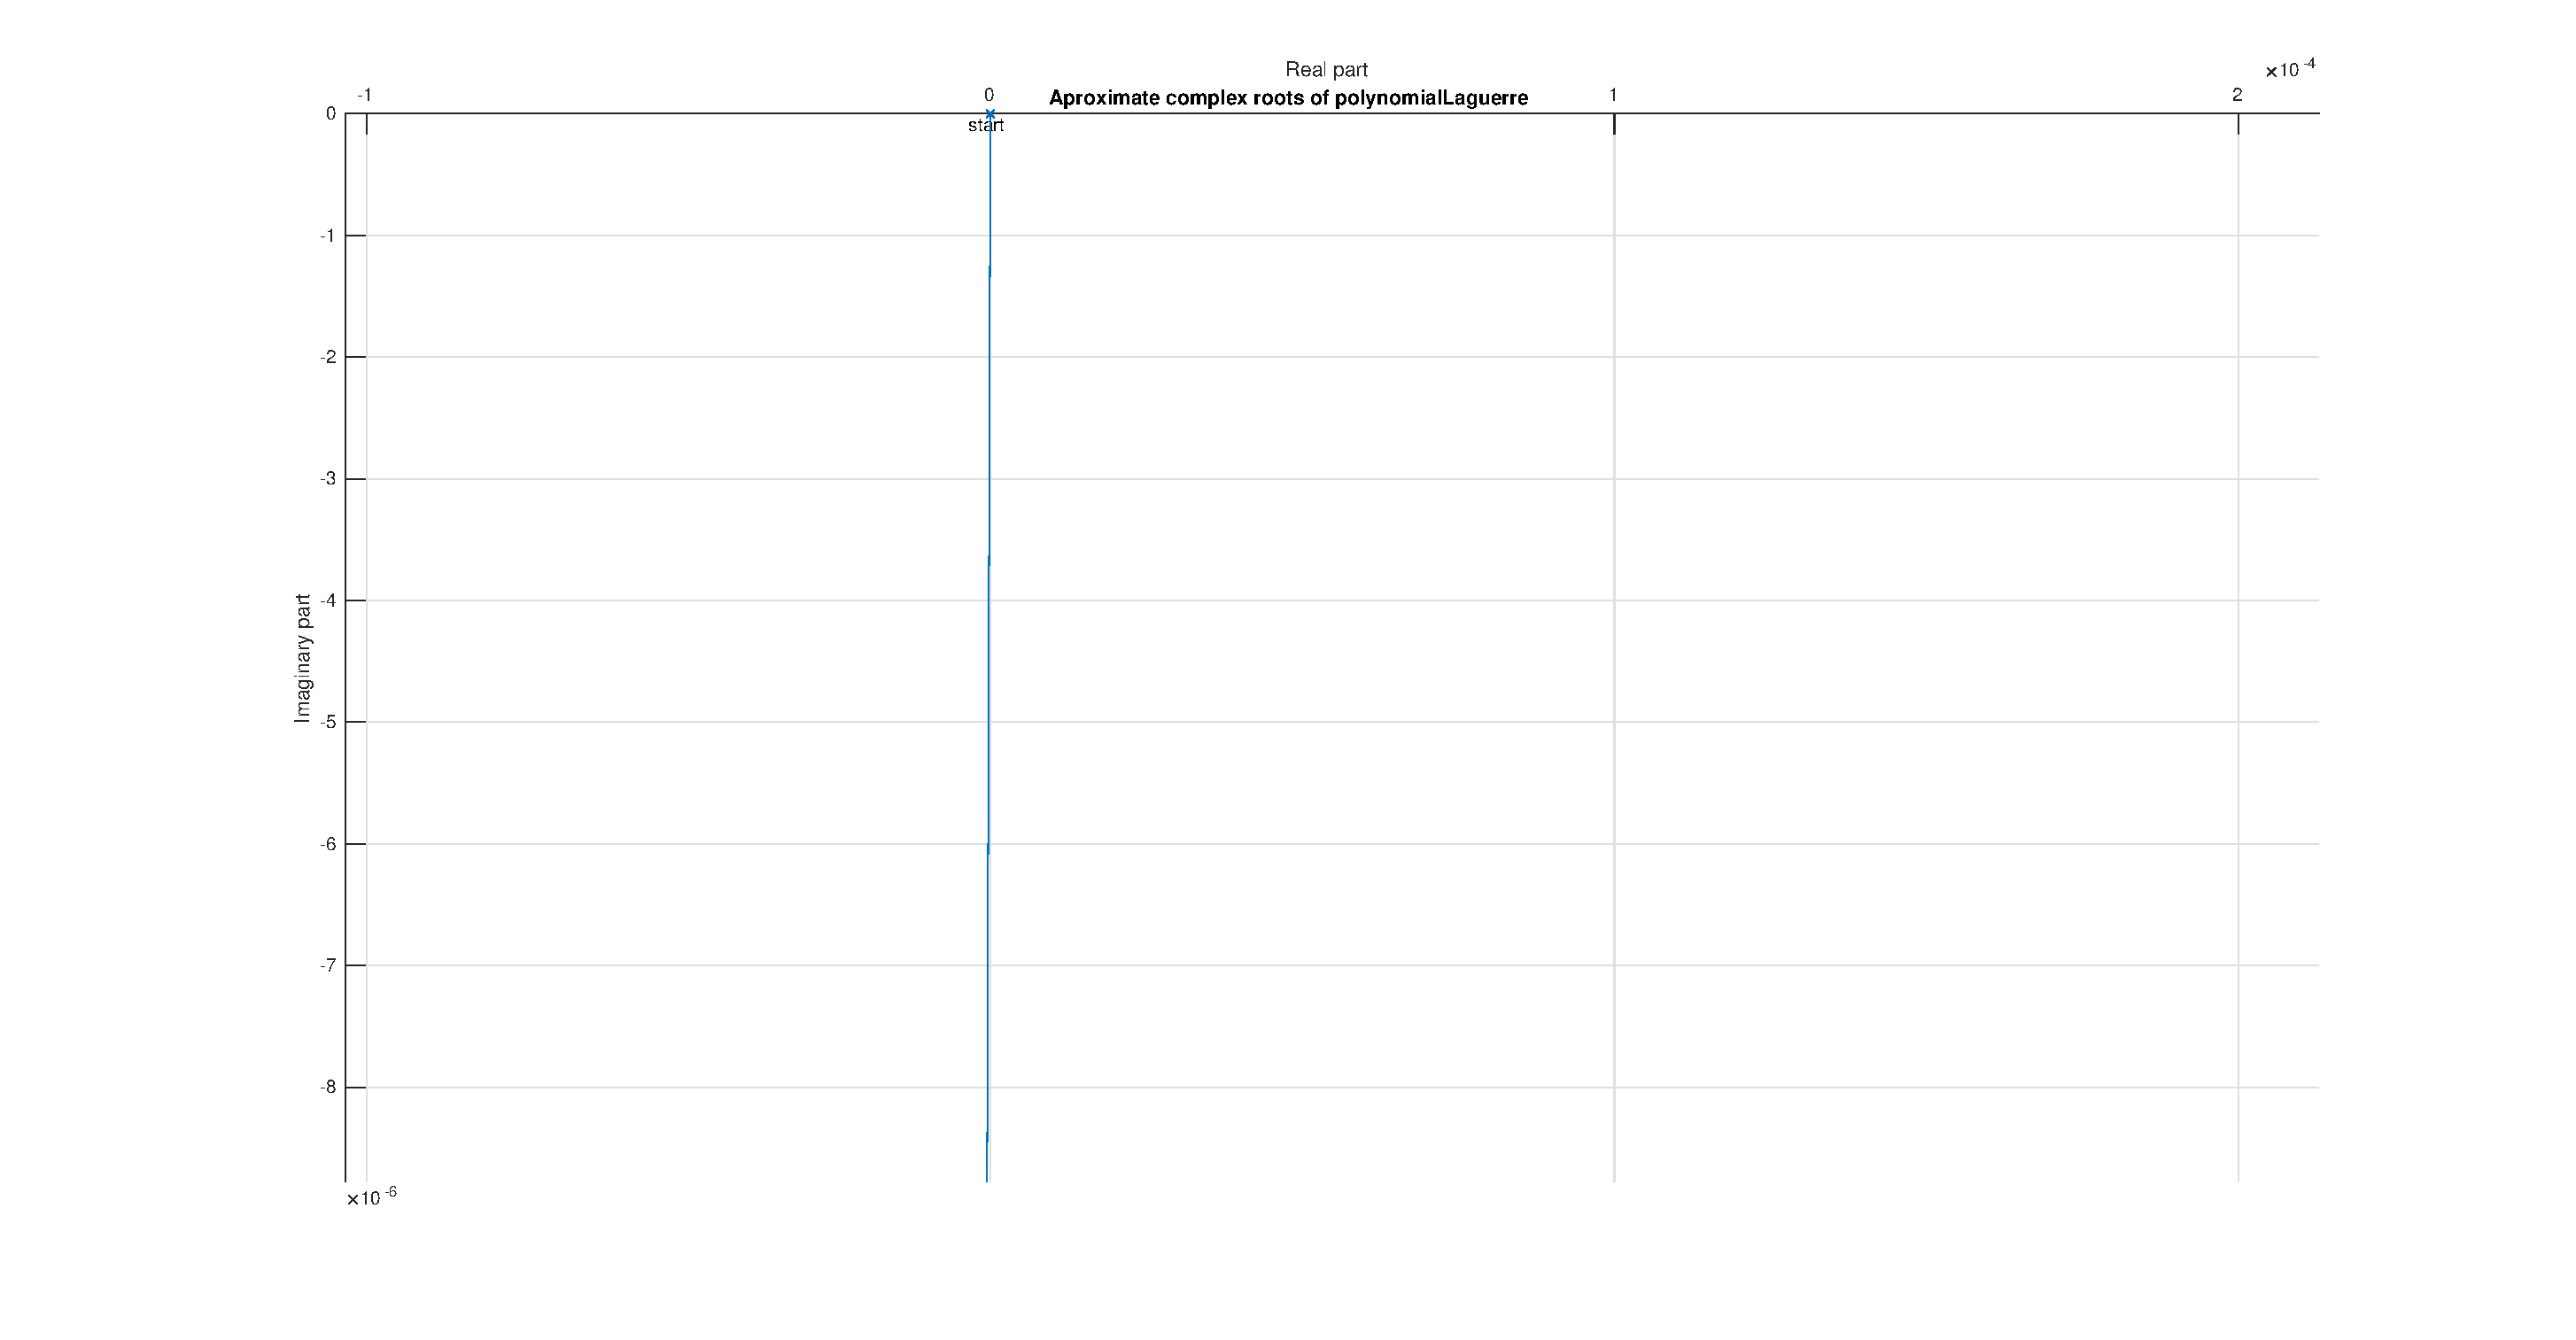
\includegraphics[scale=0.25]{task3complexup.eps}
\end{center}

\begin{center}
  \begin{tabular}{| c  c c |}
\hline
Iteration & root         & f(root) \\
\hline
1    &     -1.25   &       -20.32 \\
\hline
2    &  -0.67905   &    -0.017268 \\
\hline
3    &  -0.67787   &  -3.1489e-07 \\
\hline
4    & -0.67787    &           0 \\
\hline
\hline
\hline

\end{tabular}
\end{center}

\begin{center}
  \begin{tabular}{| c  c c |}
\hline
Iteration & root         & f(root) \\
\hline
1   &     6.25   &        43.43 \\
\hline
2   &   6.3376   &      -1.8647 \\
\hline
3   &  6.3341    &   0.0029631 \\
\hline
4   &   6.3341   &  7.9942e-09\\
\hline
5   &  6.3341    & -7.1942e-14\\
\hline


\end{tabular}
\end{center}


\begin{center}
  \begin{tabular}{| c  c c |}
\hline
Iteration & root         & f(root) \\
\hline
1   &           0+0i           &           3 \\
\hline
2   &   -0.042857+0.71586i     &      4.1826 \\
\hline
3   &       0.172+0.56266i     &    0.040584 \\
\hline
4   &    0.17188+0.56551i     &  2.8484e-06 \\
\hline
5   &     0.17188+0.56551i    &   2.2952e-14 \\
\hline
6   &     0.17188+0.56551i    &            0 \\
\hline


\end{tabular}
\end{center}


\subsection{Comparison of results between Laguerre's method and MM2 method}

\subsubsection{Tables for MM2}

\begin{center}
  \begin{tabular}{| c  c c |}
\hline
Iteration & root         & f(root) \\
\hline
1  &       -1.25+0i         &         -20.32+0i    \\
\hline
2  &    -0.72604-0.25326i   &         1.0515-4.0744i  \\
\hline
3  &   -0.68613-0.01483i    &      -0.11667-0.22303i   \\
\hline
4  &   -0.67788+2.5407e-06i &   -0.00010163+3.7123e-05i \\
\hline
5  &    -0.67787-8.0819e-13i &    1.4105e-11-1.1809e-11i \\
\hline
 \hline

\end{tabular}
\end{center}

\begin{center}
  \begin{tabular}{| c  c c |}
\hline
Iteration & root         & f(root) \\
\hline
1   &     6.25    &       43.43 \\
\hline
2   &   6.3376    &     -1.8647 \\
\hline
3   &  6.3341     &  0.0029695 \\
\hline
4   &   6.3341    &  1.6294e-08 \\
\hline
5   &   6.3341    & -4.6896e-13 \\
\hline
\hline

\end{tabular}
\end{center}

\begin{center}
  \begin{tabular}{| c  c c |}
\hline
Iteration & root         & f(root) \\
\hline
1   &         0+0i          &            3 \\
\hline
2   &    -0.125+0.85696i    &       8.0341 \\
\hline
3   &   0.16892+0.62593i    &      0.94053 \\
\hline
4   &   0.17203+0.56536i    &    0.0031354  \\
\hline
5   &   0.17188+0.56551i    &   3.8615e-09  \\
\hline
6   &   0.17188+0.56551i    &            0  \\
\hline
\hline

\end{tabular}
\end{center}

As expected Laguerre's method reigns supreme, it is:
\begin{enumerate}
\item Faster
With 5 iterations on average compared to around 5.3 for MM2
\item More accurate
For real root -0.67787 matlab calculated the value of this function for Laguerre's method as equal to exactly 0 as opposed to around $10^{-11}$ error for MM2.
\item With no errors
Laguerre's method did not mistakenly added imaginary part to real root -0.67787 as MM2 did. 
\end{enumerate}

Laguerre's method is faster and more accurate than MM2 which means that we can compare it to faster version of MM1, this means that it is the best method we tested in this exercise.

\chapter{Code appendix}

\section{Task 1}

\subsection{task1Bisection.m}

\subsubsection{Top of task1Bisection.m}
\begin{simplechar}
\begin{lstlisting}
interval = [-5, 10];
rootBrackets = rootBracketing(@taskFunction, interval(1), interval(2));

printGraph(@taskFunction, 'False Position', @falsePosition, interval, rootBrackets, 'Approximate zeros of function for method of ');
\end{lstlisting}
\end{simplechar}

\subsubsection{taskFunction}
\begin{simplechar}
\begin{lstlisting}
function y = taskFunction(x)
    y = -2.1 + 0.3*x - x*exp(1)^(-x);
end
\end{lstlisting}
\end{simplechar}

\newpage
\subsubsection{falsePosition}
\begin{simplechar}
\begin{lstlisting}
function [zero, iterations] = falsePosition(taskFunction, a, b, tolerance)

    [iterations, lastTwoA, lastTwoB, i] = initialize();
    [zero, iterations, a, b, lastTwoA, lastTwoB] = firstTwoIterations(a, b, taskFunction, iterations, lastTwoA, lastTwoB);
    [zero, iterations] = falsePositionLoop(taskFunction, zero, tolerance, lastTwoA, lastTwoB, i, a, b, iterations);
end
\end{lstlisting}
\end{simplechar}

\subsubsection{initialize}
\begin{simplechar}
\begin{lstlisting}
function [iterations, lastTwoA, lastTwoB, i] = initialize()
    iterations = double.empty(2, 0);
    lastTwoA = double.empty(2, 0);
    lastTwoB = double.empty(2, 0);
    i = 0;
end
\end{lstlisting}
\end{simplechar}

\subsubsection{taskFunction}
\begin{simplechar}
\begin{lstlisting}
function y = taskFunction(x)
    y = -2.1 + 0.3*x - x*exp(1)^(-x);
end
\end{lstlisting}
\end{simplechar}

\newpage
\subsubsection{firstTwoIterations}
\begin{simplechar}
\begin{lstlisting}
function [zero, iterations, a, b, lastTwoA, lastTwoB] = firstTwoIterations(a, b, taskFunction, iterations, lastTwoA, lastTwoB)
    for j = 1 : 2
        zero = (a*taskFunction(b) - b * taskFunction(a)) / (taskFunction(b) - taskFunction(a));
        iterations(:, size(iterations, 2) + 1) = [zero, taskFunction(zero)];
        if sign(taskFunction(a)) ~= sign(taskFunction(zero))
            b = zero;
        else
            a = zero;
        end
        lastTwoA(j) = a;
        lastTwoB(j) = b;
    end
end
\end{lstlisting}
\end{simplechar}

\subsubsection{falsePositionLoop}
\begin{simplechar}
\begin{lstlisting}
function [zero, iterations] = falsePositionLoop(taskFunction, zero, tolerance, lastTwoA, lastTwoB, i, a, b, iterations)
    while abs(taskFunction(zero)) > tolerance
        [lastTwoA, i, a, lastTwoB, b, tolerance, zero, iterations] = insideLoop(lastTwoA, i, a, lastTwoB, b, tolerance, taskFunction, iterations);
    end
end
\end{lstlisting}
\end{simplechar}

\newpage
\subsubsection{insideLoop}
\begin{simplechar}
\begin{lstlisting}
function [lastTwoA, i, a, lastTwoB, b, tolerance, zero, iterations] = insideLoop(lastTwoA, i, a, lastTwoB, b, tolerance, taskFunction, iterations)
    [lastTwoA, lastTwoB] = changeLastTwoAB(lastTwoA, lastTwoB, i, a, b);
    zero = calculateZero(lastTwoB, tolerance, a, b, lastTwoA, taskFunction);
    iterations(:, size(iterations, 2) + 1) = [zero, taskFunction(zero)];
    [a, b] = newSubInterval(taskFunction, a, b, zero);
end
\end{lstlisting}
\end{simplechar}

\subsubsection{changeLastTwoAB}
\begin{simplechar}
\begin{lstlisting}
function [lastTwoA, lastTwoB] = changeLastTwoAB(lastTwoA, lastTwoB, i, a, b)
    lastTwoA(mod(i, 2) + 1) = a;
    lastTwoB(mod(i, 2) + 1) = b;
end
\end{lstlisting}
\end{simplechar}

\newpage
\subsubsection{calculateZero}
\begin{simplechar}
\begin{lstlisting}
function [zero] = calculateZero(lastTwoB, tolerance, a, b, lastTwoA, taskFunction)
    if(abs(lastTwoB(1) - lastTwoB(2)) < tolerance)
        zero = (a*(taskFunction(b) / 2) - b * taskFunction(a)) / (taskFunction(b) / 2 - taskFunction(a));
    elseif (abs(lastTwoA(1) - lastTwoA(2)) < tolerance)
        zero = (a*taskFunction(b) - b * (taskFunction(a) / 2)) / (taskFunction(b) - (taskFunction(a) / 2));
    else
        zero = (a*taskFunction(b) - b * taskFunction(a)) / (taskFunction(b) - taskFunction(a));
    end
end
\end{lstlisting}
\end{simplechar}

\subsubsection{newSubInterval}
\begin{simplechar}
\begin{lstlisting}
function [a, b] = newSubInterval(taskFunction, a, b, zero)
    if sign(taskFunction(a)) ~= sign(taskFunction(zero))
        b = zero;
    else
        a = zero;
    end
end

\end{lstlisting}
\end{simplechar}



\subsection{task1Newton.m}

\subsubsection{Top of task1Newton.m}
\begin{simplechar}
\begin{lstlisting}
interval = [-5, 10];
rootBrackets = rootBracketing(@taskFunction, interval(1), interval(2));

printGraph(@taskFunction, 'Newton', @newtonMethod, interval, rootBrackets, 'Approximate zeros of function for method of ');
\end{lstlisting}
\end{simplechar}

\subsubsection{taskFunction}
\begin{simplechar}
\begin{lstlisting}
function y = taskFunction(x)
    y = -2.1 + 0.3*x - x*exp(1)^(-x);
end
\end{lstlisting}
\end{simplechar}

\subsubsection{newtonMethod}
\begin{simplechar}
\begin{lstlisting}
function [zero, iterations] = newtonMethod(taskFunction, a, b, tolerance)
    [iterations, iteration, zero] = initialize(a, b);
    [zero, iterations] = newtonLoop(iterations, iteration, zero, a, b, tolerance, taskFunction);
end
\end{lstlisting}
\end{simplechar}

\subsubsection{initialize}
\begin{simplechar}
\begin{lstlisting}
function [iterations, step, zero] = initialize(a, b)
    iterations = double.empty(2, 0);
    step = sqrt(eps);
    zero = (a + b) / 2;
    iterations(:, size(iterations, 2) + 1) = [zero, taskFunction(zero)];
end
\end{lstlisting}
\end{simplechar}

\subsubsection{newtonLoop}
\begin{simplechar}
\begin{lstlisting}
function [zero, iterations] = newtonLoop(iterations, iteration, zero, a, b, tolerance, taskFunction)
    while abs(taskFunction(zero)) > tolerance
        [zero, iterations] = insideLoop(taskFunction, zero, iteration, iterations, a, b);
    end
end
\end{lstlisting}
\end{simplechar}

\subsubsection{insideLoop}
\begin{simplechar}
\begin{lstlisting}
function [zero, iterations] = insideLoop(taskFunction, zero, iteration, iterations, a, b)
    [zero, iterations] = calculateZeroIterations(taskFunction, zero, iteration, iterations);
    checkForDivergence(zero, a, b);
end
\end{lstlisting}
\end{simplechar}

\subsubsection{calculateZeroIterations}
\begin{simplechar}
\begin{lstlisting}
function [zero, iterations] = calculateZeroIterations(taskFunction, zero, iteration, iterations)
    derivative = (taskFunction(zero + iteration) - taskFunction(zero - iteration)) / (2 * iteration);
    zero = zero - taskFunction(zero) / derivative;
    iterations(:, size(iterations, 2) + 1) = [zero, taskFunction(zero)];
end
\end{lstlisting}
\end{simplechar}

\subsubsection{checkForDivergence}
\begin{simplechar}
\begin{lstlisting}
function checkForDivergence(zero, a, b)
    if zero < a || zero > b
        error('Divergent iteration');
    end
end
\end{lstlisting}
\end{simplechar}

\newpage
\section{Task 2}

\subsection{task2MM1.m}

\subsubsection{Top of task2MM1}
\begin{simplechar}
\begin{lstlisting}
interval = [-5, 10];
rootBrackets = rootBracketing(@polynomial, interval(1), interval(2));

printGraph(@polynomial, 'MM1', @mm1, interval, rootBrackets, 'Approximate zeros of function for method of ');

printComplexGraph(@polynomial, 'MM1', @mm1, [-1 - i, 1 + i], 'Aproximate complex roots of polynomial');
\end{lstlisting}
\end{simplechar}

\subsubsection{polynomial}
\begin{simplechar}
\begin{lstlisting}
function y = polynomial(x)
    y = -2 * x^4 + 12 * x^3 + 4* x^2 + 1 * x + 3;
end
\end{lstlisting}
\end{simplechar}

\subsubsection{mm1}
\begin{simplechar}
\begin{lstlisting}
function [approximation, iterations] = mm1(polynomial, a, b, tolerance)
    [approximation, approximationValue, iterations] = initialize(a, b, polynomial);
    [approximation, iterations] = mm1Loop(approximation, tolerance, approximationValue, iterations, polynomial);
end
\end{lstlisting}
\end{simplechar}

\newpage
\subsubsection{initialize}
\begin{simplechar}
\begin{lstlisting}
function [approximation, approximationValue, iterations] = initialize(a, b, polynomial)
    approximation = [a, b, (a + b) / 2];
    approximationValue = arrayfun(polynomial, approximation);
    iterations = [approximation(3); polynomial(approximation(3))];
end
\end{lstlisting}
\end{simplechar}

\subsubsection{mm1Loop}
\begin{simplechar}
\begin{lstlisting}
function [approximation, iterations] = mm1Loop(approximation, tolerance, approximationValue, iterations, polynomial)
    while abs(polynomial(approximation(3))) > tolerance
        [approximation, approximationValue, iterations] = insideLoop(approximation, approximationValue, polynomial, iterations);
    end
end
\end{lstlisting}
\end{simplechar}

\subsubsection{insideLoop}
\begin{simplechar}
\begin{lstlisting}
function [approximation, approximationValue, iterations] = insideLoop(approximation, approximationValue, polynomial, iterations)
    equationsSystem = createEquationSystem(approximation, approximationValue);
    [zPlus, zMinus] = rootsOfQuadraticFormula(equationsSystem, approximationValue);
    [approximation, approximationValue, iterations] = updateApproximations(zPlus, zMinus, approximation, iterations, polynomial);
end
\end{lstlisting}
\end{simplechar}

\subsubsection{createEquationSystem}
\begin{simplechar}
\begin{lstlisting}
function equationsSystem = createEquationSystem(approximation, approximationValue)
    [z0, z1, difference0, difference1] = initializeEquationSystem(approximation, approximationValue);
    equationsSystem = solveEquationSystem(z0, difference0, z1, difference1);
end
\end{lstlisting}
\end{simplechar}

\subsubsection{rootsOfQuadraticFormula}
\begin{simplechar}
\begin{lstlisting}
function [zPlus, zMinus] = rootsOfQuadraticFormula(equationsSystem, approximationValue)
    [a, b, c] = createApproximatedQuadraticFormula(equationsSystem, approximationValue);
    [zPlus, zMinus] = findRootsOfQuadraticFormula(a, b, c);
end
\end{lstlisting}
\end{simplechar}

\subsubsection{updateApproximations}
\begin{simplechar}
\begin{lstlisting}
function [approximation, approximationValue, iterations] = updateApproximations(zPlus, zMinus, approximation, iterations, polynomial)
    newApproximation = chooseNewRoot(zPlus, zMinus, approximation);
    iterations = addZeroToIterationVector(newApproximation, iterations, polynomial);
    worstApproximationIndex = getWorstApproximationIndex(approximation, newApproximation);
    [approximation, approximationValue] = deleteWorstApproximation(worstApproximationIndex, approximation, polynomial, newApproximation);
end
\end{lstlisting}
\end{simplechar}

\subsubsection{initializeEquationSystem}
\begin{simplechar}
\begin{lstlisting}
function [z0, z1, difference0, difference1] = initializeEquationSystem(approximation, approximationValue)
    z0 = approximation(1) - approximation(3);
    z1 = approximation(2) - approximation(3);
    difference0 = approximationValue(1) - approximationValue(3);
    difference1 = approximationValue(2) - approximationValue(3);
end
\end{lstlisting}
\end{simplechar}

\subsubsection{solveEquationSystem}
\begin{simplechar}
\begin{lstlisting}
function equationsSystem = solveEquationSystem(z0, difference0, z1, difference1)
    equationsSystem = [z0 ^ 2, z0, difference0; z1 ^ 2, z1, difference1];
    reductor = equationsSystem(2, 1) / equationsSystem(1, 1);
    equationsSystem(2, :) = equationsSystem(2, :) - reductor * equationsSystem(1, :);
    equationsSystem(2, 1) = 0;
    equationsSystem(2, :) = equationsSystem(2, :) ./ equationsSystem(2, 2);
    equationsSystem(1, :) = equationsSystem(1, :) - equationsSystem(1, 2) * equationsSystem(2, :);
    equationsSystem(1, :) = equationsSystem(1, :) ./ equationsSystem(1, 1);
end
\end{lstlisting}
\end{simplechar}

\newpage
\subsubsection{createApproximatedQuadraticFormula}
\begin{simplechar}
\begin{lstlisting}
function [a, b, c] = createApproximatedQuadraticFormula(equationsSystem, approximationValue)
    a = equationsSystem(1, 3);
    b = equationsSystem(2, 3);
    c = approximationValue(3);
end
\end{lstlisting}
\end{simplechar}

\subsubsection{findRootsOfQuadraticFormula}
\begin{simplechar}
\begin{lstlisting}
function [zPlus, zMinus] = findRootsOfQuadraticFormula(a, b, c)
    zPlus = -2 * c / (b + sqrt(b ^ 2 - 4 * a * c));
    zMinus = -2 * c / (b - sqrt(b ^ 2 - 4 * a * c));
end
\end{lstlisting}
\end{simplechar}

\subsubsection{chooseNewRoot}
\begin{simplechar}
\begin{lstlisting}
function newApproximation = chooseNewRoot(zPlus, zMinus, approximation)
    if abs(zPlus) < abs(zMinus)
        newApproximation = approximation(3) + zPlus;
    else
        newApproximation = approximation(3) + zMinus;
    end
end
\end{lstlisting}
\end{simplechar}

\subsubsection{addZeroToIterationVector}
\begin{simplechar}
\begin{lstlisting}
function iterations = addZeroToIterationVector(newApproximation, iterations, polynomial)
    zero = newApproximation;
    iterations(:, size(iterations, 2) + 1) = [zero, polynomial(zero)];
end
\end{lstlisting}
\end{simplechar}

\subsubsection{getWorstApproximationIndex}
\begin{simplechar}
\begin{lstlisting}
function worstApproximationIndex = getWorstApproximationIndex(approximation, newApproximation)
    worstApproximationIndex = -1;
    worstApproximationDifference = 0;
    for i = 1:size(approximation, 2)
        diff = abs(approximation(i) - newApproximation);
        if diff > worstApproximationDifference
            worstApproximationIndex = i;
            worstApproximationDifference = diff;
        end
    end
end
\end{lstlisting}
\end{simplechar}

\subsubsection{deleteWorstApproximation}
\begin{simplechar}
\begin{lstlisting}
function [approximation, approximationValue] = deleteWorstApproximation(worstApproximationIndex, approximation, polynomial, newApproximation)
    approximation(worstApproximationIndex) = [];
    approximation(3) = newApproximation;
    approximationValue = arrayfun(polynomial, approximation);
end
\end{lstlisting}
\end{simplechar}

\newpage
\subsection{task2MM2.m}


\subsubsection{top of task2MM2.m}
\begin{simplechar}
\begin{lstlisting}
interval = [-5, 10];
rootBrackets = rootBracketing(@polynomial, interval(1), interval(2));

printGraph(@polynomial, 'MM2', @mm2, interval, rootBrackets, 'Approximate zeros of function for method of ');

printComplexGraph(@polynomial, 'MM2', @mm2, [-1 - i, 1 + i], 'Aproximate complex roots of polynomial');
\end{lstlisting}
\end{simplechar}

\subsubsection{polynomial}
\begin{simplechar}
\begin{lstlisting}
function y = polynomial(x)
    y = -2 * x^4 + 12 * x^3 + 4* x^2 + 1 * x + 3;
end

\end{lstlisting}
\end{simplechar}

\subsubsection{mm2}
\begin{simplechar}
\begin{lstlisting}
function [approximation, iterations] = mm2(polynomial, a, b, tolerance)
    [approximation, iterations] = initialize(a, b, polynomial);
    [approximation, iterations] = mm2Loop(approximation, iterations, polynomial, tolerance);
end
\end{lstlisting}
\end{simplechar}

\subsubsection{initialize}
\begin{simplechar}
\begin{lstlisting}
function [approximation, iterations] = initialize(a, b, polynomial)
    approximation = (a + b) / 2;
    iterations = [approximation; polynomial(approximation)];
end

\end{lstlisting}
\end{simplechar}

\subsubsection{mm2Loop}
\begin{simplechar}
\begin{lstlisting}
function [approximation, iterations] = mm2Loop(approximation, iterations, polynomial, tolerance)
    while abs(polynomial(approximation)) > tolerance
       [approximation, iterations] = insideLoop(approximation, polynomial, iterations);
    end
end
\end{lstlisting}
\end{simplechar}

\subsubsection{insideLoop}
\begin{simplechar}
\begin{lstlisting}
function [approximation, iterations] = insideLoop(approximation, polynomial, iterations)
        [a, b, c] = getABC(approximation, polynomial);
        [zPlus, zMinus] = findRoots(a, b, c);
        newApproximation = chooseNewApproximation(zPlus, zMinus, approximation);
        [approximation, iterations] = updateApproximations(newApproximation, iterations, polynomial);
end
\end{lstlisting}
\end{simplechar}

\subsubsection{getABC}
\begin{simplechar}
\begin{lstlisting}
function [a, b, c] = getABC(approximation, polynomial)
    c = polynomial(approximation);
    b = derivative(polynomial, approximation, 1);
    a = derivative(polynomial, approximation, 2) / 2;
end
\end{lstlisting}
\end{simplechar}

\subsubsection{findRoots}
\begin{simplechar}
\begin{lstlisting}
function [zPlus, zMinus] = findRoots(a, b, c)
    zPlus = -2 * c / (b + sqrt(b ^ 2 - 4 * a * c));
    zMinus = -2 * c / (b - sqrt(b ^ 2 - 4 * a * c));
end
\end{lstlisting}
\end{simplechar}

\subsubsection{chooseNewApproximation}
\begin{simplechar}
\begin{lstlisting}
function newApproximation = chooseNewApproximation(zPlus, zMinus, approximation)
    if abs(zPlus) < abs(zMinus)
        newApproximation = approximation + zPlus;
    else
        newApproximation = approximation + zMinus;
    end
end
\end{lstlisting}
\end{simplechar}

\subsubsection{updateApproximations}
\begin{simplechar}
\begin{lstlisting}
function [approximation, iterations] = updateApproximations(newApproximation, iterations, polynomial)
    approximation = newApproximation;
    iterations(:, size(iterations, 2) + 1) = [approximation, polynomial(approximation)];
end
\end{lstlisting}
\end{simplechar}

\subsubsection{derivative}
\begin{simplechar}
\begin{lstlisting}
function y = derivative(function_, x, degree)
    if degree == 0
        y = function_(x);
        return
    end

    step = sqrt(eps);
    y = (derivative(function_, x + step, degree - 1) - derivative(function_, x - step, degree - 1)) / (2 * step);
end
\end{lstlisting}
\end{simplechar}

\section{Task 3}

\subsubsection{Top of Task 3}
\begin{simplechar}
\begin{lstlisting}
interval = [-5, 10];
rootBrackets = rootBracketing(@polynomial, interval(1), interval(2));

printGraph(@polynomial, 'Laguerre', @laguerre, interval, rootBrackets, 'Approximate zeros of function for method of ');

printComplexGraph(@polynomial, 'Laguerre', @laguerre, [-1 - i, 1 + i], 'Aproximate complex roots of polynomial');
\end{lstlisting}
\end{simplechar}

\subsubsection{polynomial}
\begin{simplechar}
\begin{lstlisting}
function y = polynomial(x)
    y = -2 * x^4 + 12 * x^3 + 4* x^2 + 1 * x + 3;
end
\end{lstlisting}
\end{simplechar}

\subsubsection{laguerre}
\begin{simplechar}
\begin{lstlisting}
function [zero, iterations] = laguerre(polynomial, a, b, tolerance)
    [degree, zero, iterations] = initialize(a, b, polynomial);
    [zero, iterations] = laguerreLoop(polynomial, zero, tolerance, iterations, degree);

end
\end{lstlisting}
\end{simplechar}

\newpage
\subsubsection{initialize}
\begin{simplechar}
\begin{lstlisting}
function [degree, zero, iterations] = initialize(a, b, polynomial)
    degree = 4;
    zero = (a + b) / 2;
    iterations = [zero; polynomial(zero)];
end
\end{lstlisting}
\end{simplechar}

\subsubsection{laguerreLoop}
\begin{simplechar}
\begin{lstlisting}
function [zero, iterations] = laguerreLoop(polynomial, zero, tolerance, iterations, degree)
    while abs(polynomial(zero)) > tolerance
        [iterations, zero] = insideLoop(polynomial, zero, degree, iterations);
    end
end
\end{lstlisting}
\end{simplechar}

\subsubsection{insideLoop}
\begin{simplechar}
\begin{lstlisting}
function [iterations, zero] = insideLoop(polynomial, zero, degree, iterations)
    [derrivative0, derrivative1, derrivative2] = calculateDerrivatives(polynomial, zero);
    [zPlus, zMinus] = calculateZ(degree, derrivative0, derrivative1, derrivative2);
    newZero = chooseNewZero(zPlus, zMinus, zero);
    [zero, iterations] = updateZeros(newZero, iterations, polynomial);
end
\end{lstlisting}
\end{simplechar}

\newpage
\subsubsection{calculateDerrivatives}
\begin{simplechar}
\begin{lstlisting}
function [derrivative0, derrivative1, derrivative2] = calculateDerrivatives(polynomial, zero)
    derrivative0 = polynomial(zero);
    derrivative1 = derivative(polynomial, zero, 1);
    derrivative2 = derivative(polynomial, zero, 2);
end
\end{lstlisting}
\end{simplechar}

\subsubsection{calculateZ}
\begin{simplechar}
\begin{lstlisting}
function [zPlus, zMinus] = calculateZ(degree, derrivative0, derrivative1, derrivative2)
    expressionUnderSquareRoot = (degree - 1) * ((degree - 1) * derrivative1 ^ 2 - degree * derrivative0 * derrivative2);
    lagsqrt = sqrt(expressionUnderSquareRoot);

    zPlus = degree * derrivative0 / (derrivative1 + lagsqrt);
    zMinus = degree * derrivative0 / (derrivative1 - lagsqrt);
end
\end{lstlisting}
\end{simplechar}

\subsubsection{chooseNewZero}
\begin{simplechar}
\begin{lstlisting}
function newZero = chooseNewZero(zPlus, zMinus, zero)
    if abs(zPlus) < abs(zMinus)
        newZero = zero - zPlus;
    else
        newZero = zero - zMinus;
    end
end
\end{lstlisting}
\end{simplechar}

\newpage
\subsubsection{updateZeros}
\begin{simplechar}
\begin{lstlisting}
function [zero, iterations] = updateZeros(newZero, iterations, polynomial)
    zero = newZero;
    iterations(:, size(iterations, 2) + 1) = [zero, polynomial(zero)];
end
\end{lstlisting}
\end{simplechar}

\subsection{rootBrackering.m}

\subsubsection{updateZeros}
\begin{simplechar}
\begin{lstlisting}
% find the root brackets of a function within the given range
function rootBrackets = rootBracketing(givenFunction, intervalLeft, intervalRight)
    [a, b, rootBrackets, resolution] = initializeValues(intervalLeft, intervalRight);
    rootBrackets = bracketingLoop(a, b, rootBrackets, intervalRight, resolution, givenFunction);
end
\end{lstlisting}
\end{simplechar}

\newpage
\subsubsection{initializeValues}
\begin{simplechar}
\begin{lstlisting}
function [a, b, rootBrackets, resolution]  = initializeValues(intervalLeft, intervalRight)
    % define search resolution
    resolution = (intervalRight - intervalLeft) / 6;
    % The higher the value of denominator the less iterations will it take
    % to reach the roots, however in order to have nice graph showing those
    % brackets I will choose relatively small denominator - I have choosen
    % the smallest natural number that still generates brackets on a graph

    % start search at the start of the range
    a = intervalLeft;
    b = intervalLeft + resolution;
    rootBrackets = double.empty(2, 0); % initialize empty vector of size 2
end
\end{lstlisting}
\end{simplechar}

\newpage
\subsubsection{bracketingLoop}
\begin{simplechar}
\begin{lstlisting}
function rootBrackets = bracketingLoop(a, b, rootBrackets, intervalRight, resolution, givenFunction)
    while b ~= intervalRight % if the bracket can't be expanded end loop
        % if the function changes sign inside the interval that means that we passed through a root that means that a bracket has been found
        if sign(givenFunction(a)) ~= sign(givenFunction(b))
            % save bracket
            rootBrackets(:, size(rootBrackets, 2) + 1) = [a, b]; % Add the new bracket to existing ones
        end
        % check next bracket
        a = b;
        b = min(a + resolution, intervalRight);
        % Once a + resolution > intervalRight, then we will know that we
        % reached beyond the interval and we must stop
    end
end
\end{lstlisting}
\end{simplechar}

\newpage
\subsection{printGraph.m}
\begin{simplechar}
\begin{lstlisting}
% graph the real roots of a function
function printGraph(taskFunction, algorithmName, algorithm, interval, rootBrackets, plotTitle)
    figure()
    grid on; % Get y values lines
    hold on; % Retain current plot when adding new plots
    title([plotTitle, algorithmName]);
    set(gca, 'XAxisLocation', 'origin'); % Set properties of current axis
    x = interval(1):0.01:interval(2);
    % x is a vector of values between left and right interval with every value being higher by 0.01
    y = arrayfun(taskFunction, x); % We sketch the function from task for each x
    plot(x, y);

    % iterate over rootBrackets and add them to the plot
    for rootBracket = rootBrackets
        % find all zeros within the bracket using the given algorithm
        % Get all steps from the algorithm we use
        [~, steps] = algorithm(taskFunction, rootBracket(1), rootBracket(2), 1e-10);

        firstStepColor = [1 0 0]; % Red
        otherStepsColor = 	[0 1 0]; % Green
        % plot first steps
        scatter(steps(1, 1), steps(2, 1), [], firstStepColor);
        text(steps(1, 1), steps(2, 1), 'firstStep', 'HorizontalAlignment', 'center', 'VerticalAlignment', 'top'); % It makes text appear neatly
        % plot other steps
        scatter(steps(1, 2:end), steps(2, 2:end), [], otherStepsColor);



    % print root table
    disp([plotTitle, ' (', algorithmName, ')']);
    columns = {'step', 'root', 'value at root'};
    disp(table((1:size(steps, 2))', steps(1, :)', steps(2, :)', 'VariableNames', columns));
    end
end

\end{lstlisting}
\end{simplechar}

\newpage
\subsection{printComplexGraph.m}
\begin{simplechar}
\begin{lstlisting}
% graph the complex roots of a function
function printComplexGraph(printComplexGraph, algorithmName, algorithm, rootBrackets, plottitle)
    figure();
    grid on; % Get y values lines
    hold on; % Retain current plot when adding new plots
    title([plottitle, algorithmName]);
    xlabel("Real part");
    ylabel("Imaginary part");
    set(gca, 'XAxisLocation', 'origin'); % Set properties of current axis

    % find all zeros within the bracket using the given algorithm
    [~, steps] = algorithm(printComplexGraph, rootBrackets(1), rootBrackets(2), 1e-15);

    % plot first step
    text(real(steps(1, 1)), imag(steps(1, 1)), 'start', 'HorizontalAlignment', 'center', 'VerticalAlignment', 'top');

    % plot steps on graph
    plot(real(steps(1, :)), imag(steps(1, :)), '-x');

    % plot last step
    text(real(steps(1, end)), imag(steps(1, end)), 'end', 'HorizontalAlignment', 'center', 'VerticalAlignment', 'top');


    % print root table
    disp([plottitle, ' (', algorithmName, ')']);
    columns = {'step', 'root', 'abs value at root'};
    disp(table([1:size(steps, 2)]', steps(1, :)', abs(steps(2, :))', 'VariableNames', columns));
end
\end{lstlisting}
\end{simplechar}


\begin{thebibliography}{9}
\bibitem{texbook}
Piotr Tatjewski (2014) \emph{Numerical Methods}, Oficyna Wydawnicza Politechniki Warszawskiej
\end{thebibliography}


\end{document}
